\documentclass[11pt,letterpaper]{article}

% Compile with: xelatex main.tex; bibtex main; xelatex main.tex; xelatex main.tex
% xelatex natively understands UTF-8, no inputenc needed.

\usepackage[margin=1in]{geometry}
\usepackage{fontspec}            % xelatex font selection
\usepackage{amsmath,amssymb,amsthm}
\usepackage{graphicx}
\usepackage{xcolor}
\usepackage{hyperref}
\usepackage[numbers,sort&compress]{natbib}
\usepackage{booktabs}
\usepackage{caption}
\usepackage{longtable}
\usepackage{array}
\usepackage{calc}
% pandoc emits \real{0.2} etc. inside table column specs; provide it.
\providecommand{\real}[1]{#1}
\providecommand{\tightlist}{\setlength{\itemsep}{0pt}\setlength{\parskip}{0pt}}
% pandoc emits \def\LTcaptype{none} to suppress table captions; define the
% counter so longtable doesn't error.
\newcounter{none}
\usepackage{microtype}
\usepackage{titlesec}
\usepackage{newunicodechar}
\usepackage{url}
% Allow line-breaks inside \url{} / \path{} at slashes, underscores,
% dots, hyphens. Output keeps typewriter font.
\PassOptionsToPackage{hyphens}{url}
% No stretchy spacing at break points — keeps path characters tight when
% the line is justified. Breaks are still enabled by \UrlBreaks below.
\Urlmuskip=0mu\relax
% Add break-points after / _ . - so file paths split cleanly.
\renewcommand{\UrlBreaks}{\do\/\do\_\do\.\do\-\do\&\do\?\do\=\do\,\do\;}
% Loosen TeX's line-breaking globally, to absorb any remaining overflow.
\sloppy
\setlength{\emergencystretch}{3em}

% Unicode -> math/text mappings (so utf8 source compiles with pdflatex)
% Greek letters
\newunicodechar{ρ}{\ensuremath{\rho}}
\newunicodechar{μ}{\ensuremath{\mu}}
\newunicodechar{σ}{\ensuremath{\sigma}}
\newunicodechar{ξ}{\ensuremath{\xi}}
\newunicodechar{α}{\ensuremath{\alpha}}
\newunicodechar{β}{\ensuremath{\beta}}
\newunicodechar{γ}{\ensuremath{\gamma}}
\newunicodechar{η}{\ensuremath{\eta}}
\newunicodechar{δ}{\ensuremath{\delta}}
\newunicodechar{ε}{\ensuremath{\varepsilon}}
\newunicodechar{τ}{\ensuremath{\tau}}
\newunicodechar{π}{\ensuremath{\pi}}
\newunicodechar{Φ}{\ensuremath{\Phi}}
\newunicodechar{Δ}{\ensuremath{\Delta}}
% Math operators / scripts
\newunicodechar{²}{\ensuremath{^{2}}}
\newunicodechar{³}{\ensuremath{^{3}}}
\newunicodechar{⁰}{\ensuremath{^{0}}}
\newunicodechar{¹}{\ensuremath{^{1}}}
\newunicodechar{⁴}{\ensuremath{^{4}}}
\newunicodechar{⁵}{\ensuremath{^{5}}}
\newunicodechar{⁶}{\ensuremath{^{6}}}
\newunicodechar{⁷}{\ensuremath{^{7}}}
\newunicodechar{⁸}{\ensuremath{^{8}}}
\newunicodechar{⁹}{\ensuremath{^{9}}}
\newunicodechar{ⁿ}{\ensuremath{^{n}}}
\newunicodechar{⁻}{\ensuremath{^{-}}}
\newunicodechar{ₑ}{\ensuremath{_{\mathrm{e}}}}
\newunicodechar{ᶜ}{\ensuremath{^{c}}}
\newunicodechar{₀}{\ensuremath{_{0}}}
\newunicodechar{₊}{\ensuremath{_{+}}}
\newunicodechar{₋}{\ensuremath{_{-}}}
\newunicodechar{√}{\ensuremath{\sqrt{\,}}}
\newunicodechar{×}{\ensuremath{\times}}
\newunicodechar{−}{\ensuremath{-}}
\newunicodechar{→}{\ensuremath{\rightarrow}}
\newunicodechar{≤}{\ensuremath{\leq}}
\newunicodechar{≥}{\ensuremath{\geq}}
\newunicodechar{≈}{\ensuremath{\approx}}
\newunicodechar{∈}{\ensuremath{\in}}
\newunicodechar{∞}{\ensuremath{\infty}}
\newunicodechar{·}{\ensuremath{\cdot}}
\newunicodechar{±}{\ensuremath{\pm}}
\newunicodechar{∝}{\ensuremath{\propto}}
\newunicodechar{∧}{\ensuremath{\wedge}}
\newunicodechar{∨}{\ensuremath{\vee}}
\newunicodechar{∑}{\ensuremath{\sum}}
\newunicodechar{≠}{\ensuremath{\neq}}
\newunicodechar{≫}{\ensuremath{\gg}}
\newunicodechar{≪}{\ensuremath{\ll}}
% Subscript Latin letters (used in symbols like h_max, J_eff, c_log)
\newunicodechar{ₐ}{\ensuremath{_{a}}}
\newunicodechar{ₓ}{\ensuremath{_{x}}}
\newunicodechar{ₖ}{\ensuremath{_{k}}}
\newunicodechar{ₘ}{\ensuremath{_{m}}}
\newunicodechar{ₚ}{\ensuremath{_{p}}}
\newunicodechar{ₛ}{\ensuremath{_{s}}}
\newunicodechar{ₜ}{\ensuremath{_{t}}}
\newunicodechar{ⱼ}{\ensuremath{_{j}}}
\newunicodechar{≳}{\ensuremath{\gtrsim}}
\newunicodechar{≲}{\ensuremath{\lesssim}}
\newunicodechar{⌊}{\ensuremath{\lfloor}}
\newunicodechar{⌋}{\ensuremath{\rfloor}}
\newunicodechar{⟨}{\ensuremath{\langle}}
\newunicodechar{⟩}{\ensuremath{\rangle}}
\newunicodechar{ℓ}{\ensuremath{\ell}}
% Punctuation
\newunicodechar{§}{\S{}}
\newunicodechar{°}{\textdegree}
\newunicodechar{…}{\ldots}
% Phonetic / IPA / specialty (best-effort fallbacks)
\newunicodechar{ˡ}{\ensuremath{^{l}}}
\newunicodechar{ˣ}{\ensuremath{^{x}}}
\newunicodechar{̄}{}
\newunicodechar{ᐟ}{}
\newunicodechar{ᴅ}{D}
\newunicodechar{ᵒ}{\ensuremath{^{o}}}
\newunicodechar{ᵢ}{\ensuremath{_{i}}}
\newunicodechar{ᵦ}{\ensuremath{_{\beta}}}
\newunicodechar{ő}{\H{o}}

\hypersetup{
  colorlinks=true,
  linkcolor=blue!50!black,
  citecolor=blue!50!black,
  urlcolor=blue!50!black,
}

\titleformat*{\section}{\Large\bfseries}
\titleformat*{\subsection}{\large\bfseries}
\titleformat*{\subsubsection}{\normalsize\bfseries\itshape}

\setlength{\parskip}{4pt}
\setlength{\parindent}{0pt}

\title{Why Fixed Protections Fail Under Rising Coordination:\\
A Structural Failure-Mode Transition in Coupled Systems}
\author{Chowon Jung\\
\small\texttt{dancing4am@gmail.com}}
\date{\today}

\begin{document}
\maketitle

\section{Abstract}\label{abstract}

Rising coordination is tightening the coupling between once-independent agents. Governance relies on passive stabilizers (diversification, constitutional checks, automatic income supports) that buffer shocks at fixed strength. We identify a structural prediction unique to coordination dynamics: as coupling rises, the \emph{type} of failure transitions from fragmentation to rigidity. This is confirmed in 22 years of S\&P 500 data --- drawdown-period correlation rises 0.50 → 0.88 across coupling deciles, rigidity share 0\% → 100\%, with empirical--model rank correlation ρ = +0.92. The underlying scaling law: a fixed field \emph{h} opposing coupling \emph{J} loses effectiveness as \emph{h}/\emph{J}² with an irreducible residual. The pattern survives across alternative model classes, topologies, and a second domain (cryptocurrency, 64\% supercritical vs \textasciitilde25\% equities). An active stabilizer eliminates the residual. A heuristic AI coupling proxy (14 models × 805 prompts) locates frontier AI in the regime where passive protections decay. Overcoming the asymmetry requires active stabilizers.

\section{Introduction}\label{introduction}

A defining feature of the current decade is rising coordination across sociotechnical systems. Algorithmic systems are pulling once-independent decisions into common alignment: high-frequency traders co-execute on shared signals, recommender feeds homogenize political opinion, large language models are converging on a small set of evaluative standards, and global supply chains route through shared infrastructure that links demand shocks across continents. The empirical signature is a tightening of cross-domain correlation. Pairwise correlations among S\&P 500 sectors exceeded 0.9 during both the March 2020 selloff and the 2010--12 Eurozone crisis (see Results). Political identity, media consumption, and consumer preference are coupling at decadal-record levels \cite{levitskyziblatt2018,svolik2019}. Mass-extinction rates exceed background by tens to hundreds of times \cite{ipbes2019,barnosky2011} despite high baseline biodiversity, because the dominant ecological stressor --- anthropogenic climate forcing --- is correlated across all species and habitats. In each domain, agents that used to fail independently are starting to fail together.

The institutional response to this trend has so far extended mechanisms designed for the previous era. Financial regulators tighten Value-at-Risk models and circuit-breaker thresholds; democracies bolster constitutional checks; conservation programs expand species inventories; nascent AI governance frameworks --- the EU AI Act's risk tiers, NIST's AI Risk Management Framework, and voluntary commitments by the Frontier Model Forum --- add audit requirements and capability thresholds. These mechanisms share a structural property that distinguishes them from a different class of intervention. They buffer shocks at a \emph{fixed} strength baked into the system's architecture, rather than scaling their response to the magnitude of any particular threat. Diversification holds the same allocation whether market correlation is 0.3 or 0.9. A circuit breaker triggers at the same 7\% threshold whether one asset is dropping or a thousand are. Constitutional separation of powers does not become structurally stronger during an authoritarian push. We term mechanisms of this kind passive stabilizers --- fixed structural protections, automatic and state-independent --- to distinguish them from active stabilizers whose response magnitude scales with measured stress (central-bank interventions, emergency fiscal stimulus, military or diplomatic action).

Whether passive stabilization remains adequate under rising coupling is, we argue, the central open question of AI-era governance. We identify a structural prediction unique to coordination dynamics --- as coupling rises, the \emph{type} of failure transitions from fragmentation to rigidity --- and confirm it in 22 years of S\&P 500 data (Spearman ρ = +0.92 against the model's type-composition). Underlying the transition is a quantitative scaling law: passive stabilizer effectiveness scales as \emph{h}/\emph{J}² and becomes structurally insufficient at high coupling.

\subsection{Domain-specific evidence and the missing substrate}\label{domain-specific-evidence-and-the-missing-substrate}

The phenomenon of passive-stabilizer failure under high coupling has been described repeatedly in domain-specific terms: diversification benefits collapse when correlations rise \cite{angchen2002,longinsolnik2001,patton2006}; circuit breakers can accelerate crashes they are designed to interrupt \cite{chen2024,sifatmohamad2019}; constitutional checks fail under synchronized opinion \cite{levitskyziblatt2018,svolik2019}; mass-extinction rates exceed background despite high biodiversity because the dominant stressor is correlated across species \cite{ipbes2019,barnosky2011}. These literatures share a missing common substrate: no quantitative scaling law connecting coupling to protection effectiveness, and no formal distinction between mechanisms that scale their response with the threat and those that do not.

\subsection{Closest existing frameworks and what they miss}\label{closest-existing-frameworks-and-what-they-miss}

The closest prior frameworks are Daníelsson's endogenous-risk theory \cite{danielsson2002,danielsson2013} and the parallel liquidity-funding spiral \cite{brunnermeier2009}; Ashby's Law of Requisite Variety \cite{ashby1956,muhlert2026}; Perrow's \emph{Normal Accidents} \cite{perrow1984}; Svolik's polarization--democracy tradeoff \cite{svolik2019}; and the asymmetric-dependence literature in finance \cite{angchen2002,longinsolnik2001}. Each captures a domain-specific version of the phenomenon without the cross-domain scaling law, without the \emph{h}/\emph{J}² quantification, and without the active/passive distinction. A detailed comparison is in Supplementary Information §S7.

\subsection{Contribution}\label{contribution}

Our contribution is fourfold. \emph{First}, we make the active/passive stabilizer distinction mathematically precise (Definition 1, Results): a \emph{passive stabilizer} has intervention magnitude bounded above by a structural constant independent of \emph{J}, stress level, and time; an \emph{active stabilizer} has magnitude that scales with the threat. Diversification, constitutional checks, biodiversity, and the income-multiplier feedback satisfy the passive definition; Federal Reserve rate cuts, emergency fiscal stimulus, and military intervention exemplify the active class. \emph{Second}, we derive a quantitative scaling law: in any system where a fixed field \emph{h} opposes a coupling \emph{J}, the field's protective effect scales as \emph{h}/\emph{J}² and decays asymptotically. The derivation is a standard consequence of Curie--Weiss free-energy structure, but to our knowledge has not been extracted as a governance principle. \emph{Third}, we confirm the scaling law in a 9,000-run sweep of a minimal two-equation simulation, and show via an ablation cascade that adding belief and credit dynamics monotonically \emph{worsens} the asymmetry --- the minimal model is the most optimistic case, not a toy that overstates. A matched-seed active-stabilizer experiment confirms the converse: replacing the bounded passive field with a stress-responsive or coupling-responsive analogue of finite strength eliminates the high-coupling residual entirely (Figure 5), demonstrating that the classification has predictive content. An agent-based extension on six network topologies (complete, Erdős--Rényi, Watts--Strogatz, Barabási--Albert, modular, modular-boundary) shows that the scaling is topology-independent --- all six topologies converge to a residual in the same 0.33--0.37 band at the headline cell, with no pair statistically separated (Figure 3). A complementary ramp-speed experiment characterizes a non-monotone speed-of-onset effect that materially refines the policy implications. \emph{Fourth}, we test the model's mechanism empirically. The headline finding is the \textbf{failure-mode transition} the framework uniquely predicts: as coupling rises, the \emph{type} of failure changes from fragmentation to rigidity. In 22 years of S\&P 500 sector data, drawdown-period correlation rises 0.50 → 0.88 across coupling deciles, rigidity share 0\% → 100\%, with empirical--model rank correlation ρ = +0.92 (Figure 7). No generic correlation-risk model makes this type-of-failure prediction. The frequency test confirms the same coupling axis: tail-risk and VaR exceedance track the model at Spearman ρ = 0.81 and 0.87, cross-mechanism ρ = 0.98 (Figure 6). A heuristic AI proxy on 805 shared prompts \cite{li2023alpacaeval} locates frontier AI above the model's critical threshold \emph{J}ᶜ = 2 --- the substantive claim is regime-placement; the precise \emph{J} depends on a non-calibrated mapping (Figure 8, SI §S8).

The ingredients are individually known; the contribution lies in their combination and governance interpretation.

\section{Results}\label{results}

\subsection{The minimal model and a scaling law for passive stabilizers}\label{the-minimal-model-and-a-scaling-law-for-passive-stabilizers}

We study the simplest dynamical system containing the two ingredients common to every example in the Introduction: a coordinated state variable subject to tunable coupling, and a fixed structural feature opposing synchronization. Let \emph{m}(\emph{t}) ∈ (--1, 1) be a mean-field coordination order parameter and \emph{W}(\emph{t}) the system's economic wealth. The minimal model is


\begin{equation*}
\dot m = -m + \tanh\!\left(\frac{J\,m + h(W)}{T}\right) + \xi\,\sqrt{1-m^2}\,\eta(t), \tag{1}
\end{equation*}



\begin{equation*}
\dot W = \mu \cdot \mathrm{employment}(m) - \mathrm{consumption}(W), \tag{2}
\end{equation*}


with employment(\emph{m}) = (1+\emph{m})/2, consumption(\emph{W}) = 30 + 10·(\emph{W}/500), and the passive stabilizer field \emph{h}(\emph{W}) = 2·(\emph{W}/500). The temperature \emph{T} = 2 sets the noise scale, \emph{ξ} = 0.5 the noise amplitude, and \emph{η}(\emph{t}) is white noise (Itô convention; see Methods). The coupling \emph{J} ∈ {[}0.5, 5{]} tunes the pull toward synchronized \emph{m} ≈ ±1, and the income multiplier \emph{μ} ∈ {[}20, 100{]} tunes the rate at which the wealth-driven field \emph{h} grows. Equation 1 is a Curie--Weiss SDE in the order parameter; Equation 2 is a deterministic wealth balance --- no Hawkes processes, Lotka--Volterra terms, demographic dynamics, credit cycle, or endogenous beliefs. Two coupled equations, six parameters, one source of stochasticity.

We identify \emph{h} as the \emph{passive stabilizer}. We define the class formally on the basis of the \emph{intervention magnitude}, not the functional form of the rule:

\textbf{Definition 1.} \emph{A} passive stabilizer \emph{is a mechanism entering the system dynamics whose intervention magnitude is bounded above by a constant independent of the system state and the coupling level. Specifically:} - \emph{(i) its maximum restoring force h}ₘₐₓ \emph{is fixed --- determined by structural parameters alone, not by the current coupling J, the current stress level, or the time t;} - \emph{(ii) it enters the dynamics as a restoring force favoring a particular equilibrium.}

\emph{An} active stabilizer \emph{is a mechanism whose intervention magnitude is itself a function of the system state, h = g(m, J, t), with g unbounded as stress increases.}

The distinction turns on the intervention's \emph{output} magnitude, not on whether the rule has fixed coefficients. The Taylor Rule's coefficients are fixed, but its rate-cut output scales with the output gap; a circuit breaker halts trading for 15 minutes regardless of move size, and diversification is bounded by 1/√\emph{N} regardless of correlation level. The criterion is boundedness of the restoring force.

In Equation 1, \emph{h}(\emph{W}) = 2·(\emph{W}/500) realizes a passive stabilizer: the conversion rate from wealth to restoring force is fixed at 2/500, and the field is bounded above by the equilibrium wealth (itself bounded by \emph{μ}). Wealth itself responds to the coupling indirectly --- high \emph{J} locks \emph{m}, which shifts employment, which shifts wealth --- but the conversion rule from \emph{W} to \emph{h} does not, and so the maximum restoring force does not scale with the threat. Diversification, constitutional checks, biodiversity, and the income-multiplier feedback in macroeconomic models each satisfy Definition 1 with a different state variable supplying \emph{h} through a fixed conversion rule. The minimal model contains no active stabilizer.

The following result is a standard consequence of the Curie--Weiss free-energy structure; we state it explicitly because, to our knowledge, it has not been extracted as a governance principle or connected to the active/passive stabilizer distinction.

\textbf{Theorem 1} (\emph{h}/\emph{J}² \emph{scaling of passive stabilizer effectiveness}). \emph{In the deterministic mean-field limit of Equations 1--2, the preferential stability of the protective (+m) branch over the unprotective (--m) branch scales as h/J² for J ≫ T. The passive stabilizer's ability to steer the system toward the productive equilibrium therefore vanishes at high coupling.}

Intuitively: at high \emph{J}, the saturated fixed points sit at \emph{m} ≈ ±1; \emph{h} tilts the landscape between branches by ≤ 2\emph{h} (independent of \emph{J}) while the protective basin narrows as 1/\emph{J}; the tilt-to-barrier ratio decays as \emph{h}/\emph{J}². Because \emph{h} is bounded by the equilibrium wealth (itself bounded by \emph{μ}), passive stabilization vanishes at high coupling regardless of \emph{μ}. Full derivation in Methods and SI.

Theorem 1 generates two qualitative predictions. First, at high \emph{J}, no attainable value of \emph{h} fully eliminates collapse --- the residual collapse rate saturates above zero. Second, the residual collapses at high \emph{J} should be \emph{rigidity-typed} (\textbar{}\emph{m}\textbar{} near 1 at the moment of failure, the system trapped on the unprotective branch) rather than \emph{fragmentation-typed} (\textbar{}\emph{m}\textbar{} near 0, the system disordered and unable to coordinate productive activity).

We tested both predictions with a 9,000-run sweep over \emph{J} ∈ \{0.5, 1.0, \ldots, 5.0\} and \emph{μ} ∈ \{20, 30, \ldots, 100\}, with 100 independent seeds per cell and 20,000 Euler--Maruyama steps per run at d\emph{t} = 0.05 (full numerical protocol in Methods). A run is classified as \emph{collapsed} if its wealth falls below 10 (10\% of the initial value) for 200 consecutive steps (10 physical time units). The collapse criterion is chosen to be unambiguously catastrophic within the model's dynamics --- representing sustained economic failure below any plausible recovery margin, not a transient downturn. The mapping from this model-internal threshold to specific real-world event categories (recession, financial crisis, civilizational breakdown) is a calibration question deferred to future work. A collapse is \emph{rigidity-typed} if \textbar{}\emph{m}\textbar{} \textgreater{} 0.9 at the collapse instant and \emph{fragmentation-typed} if \textbar{}\emph{m}\textbar{} \textless{} 0.3. The choice of d\emph{t} = 0.05 follows from a convergence check across d\emph{t} ∈ \{0.1, 0.05, 0.025\} (see Methods) showing that P(collapse) saturates at d\emph{t} ≤ 0.05.

Both predictions are confirmed (Figure 1). At the lowest coupling (\emph{J} = 0.5), the passive stabilizer eliminates collapse entirely as \emph{μ} rises from 20 to 100: P(collapse) drops from 1.00 to 0.00. In the highest coupling band (\emph{J} ≥ 4.0), the same stabilizer range only reduces P(collapse) from 1.00 to 0.23 --- a residual that does not vanish. Of the residual collapses at maximum stabilizer, 90\% are rigidity-typed under multiplicative noise (SI §S5.1: additive noise shifts the balance toward fragmentation). The two failure modes are spatially separated in the (\emph{J}, \emph{μ}) plane: fragmentation occupies the low-\emph{J}, low-\emph{μ} corner, while rigidity dominates the high-\emph{J} band at every \emph{μ}.

The minimal model exhibits exactly the structural pattern Theorem 1 predicts: passive stabilization protects against fragmentation but not against rigidity, where synchronized lock-in cannot be overridden by bounded passive intervention. The 23\% high-\emph{J} residual at maximum \emph{μ} is the finite-noise, finite-\emph{h} signature of the \emph{h}/\emph{J}² → 0 scaling.

\subsection{Robustness: an ablation cascade}\label{robustness-an-ablation-cascade}

The minimal model omits dynamical elements commonly invoked in the socio-economic instability literature --- endogenous belief dynamics, credit cycles, demographic feedback. We tested whether the asymmetry result is a structural artifact of those omissions with an ablation cascade: identical (\emph{J}, \emph{μ}) sweep, seeds, and integration protocol, adding complexity one level at a time.

\textbf{Level 0} is the bare Curie--Weiss SDE with fixed exogenous \emph{h}; its long-time mean matches the mean-field fixed-point analysis underlying Theorem 1 (Supplementary Figure S1). \textbf{Level 1} is the minimal model (residual 23\% at \emph{μ} = 100, 90\% rigidity). \textbf{Level 2} adds replicator--mutator dynamics over \emph{K} = 6 belief types with epistemic-coherence factor \emph{h}ₑff = \emph{h}·EC (Methods): residual \textbf{30\%}, rigidity 83\%. \textbf{Level 3} adds Minsky--Keen credit-cycle dynamics: residual \textbf{34\%}, rigidity 81\%. \textbf{Level 4} is the full simulator (belief + credit + Hawkes shocks + Lotka--Volterra + demographics + mortality) reported from prior work at d\emph{t} = 0.1: 30--35\% band, rigidity dominates; not re-run at d\emph{t} = 0.05 (SI §S1.3).

Across L1 → L2 → L3 at consistent d\emph{t} = 0.05 the residual increases monotonically (Figure 2; 23\% → 30\% → 34\%) with rigidity dominance preserved (90\%, 83\%, 81\%). L4 (full simulator from prior work, run at d\emph{t} = 0.1) reports residuals in the 30--35\% band, consistent with the L1--L3 trend; we do not re-establish strict monotonicity through L4 here, but its residual is within the L1--L3 envelope and adds no counterevidence. The minimal model is the most optimistic case across the tested cascade.

\subsection{Network robustness: the scaling law beyond mean-field}\label{network-robustness-the-scaling-law-beyond-mean-field}

A natural concern about mean-field is that modular network structure might restore passive-stabilizer effectiveness by decoupling communities. We tested this with an agent-based extension: N = 200 agents on six graph topologies --- complete (mean-field control), Erdős--Rényi, Watts--Strogatz, Barabási--Albert, planted-partition modular (4 communities), and modular with stabilizer applied only at community boundaries --- same Curie--Weiss local dynamics, wealth feedback, sweep grid, and collapse criteria as the scalar model (Methods).

The \emph{h}/\emph{J}² scaling survives on every tested topology (Figure 3). At the headline cell (\emph{J} = 5, \emph{μ} = 100), a 100-seed re-run (SI §S9) finds all six topologies converge to P(collapse) ∈ {[}0.33, 0.37{]}, with no pair separated above one standard error (largest gap: boundary-localized 0.37 vs.~complete 0.33, Z ≈ 0.59 in a two-sample test of proportions). \textbf{None} of the six tested topologies --- complete, Erdős--Rényi, Watts--Strogatz, Barabási--Albert, modular, or boundary-localized --- rescues the mean-field residual. Intra-community and inter-community trajectory correlations both reach 1.00 at high \emph{J}: the entire network synchronizes despite only \textasciitilde1\% inter-community edge density. The mean-field prediction holds across every tested topology.

\subsection{Dynamic coupling: speed-of-onset asymmetry}\label{dynamic-coupling-speed-of-onset-asymmetry}

Real-world coupling does not jump between fixed values. The minimal model accommodates time-varying coupling by replacing the static \emph{J} with a schedule \emph{J}(\emph{t}). We tested three canonical schedules: a \emph{gradual} linear ramp from \emph{J} = 0.5 to \emph{J} = 5.0 over the simulation horizon; an \emph{exponential} S-curve representing late-saturating adoption; and a \emph{sudden} step function modeling a discrete capability gain.

Across 100 seeds × 9 \emph{μ} levels × 3 schedules × 30,000 steps (d\emph{t} = 0.05), the gradual and exponential schedules survive at every margin \emph{μ} ≥ 60 (P(collapse) ≤ 3\%), whereas sudden onset triggers rigidity collapse across the band (P(collapse) = 47\% at \emph{μ} = 40, declining to 2\% at \emph{μ} = 80; rigidity dominates the residual at every margin tested --- ≥ 77\%, 77--100\% in cells with \emph{n} ≥ 10 collapses).

The mechanism is \emph{adiabatic settling}: gradual ramps build \emph{h} before \emph{J} binds, entering Theorem 1's regime on the protective branch; sudden onset lets noise select the branch.

A ramp-duration sweep over six durations from 1,000 to 30,000 steps (5,400 runs) reveals three regimes (Figure 4): \emph{resilient} (\emph{μ} ≥ 60, P(collapse) ≤ 7\% at every ramp duration); \emph{critical} (\emph{μ} = 50, P(collapse) monotonically increasing from 0.19 to 0.49; 50\% threshold near 9,200 steps); \emph{unviable} (\emph{μ} ≤ 40, P(collapse) saturates at 1.00 by ramp ≈ 4,000 steps). The collapse-type composition swaps: fast ramps produce a partly rigidity-typed residual, while slow ramps at low margin produce an overwhelmingly fragmentation-typed residual.

Slow deployment protects high-margin economies through adiabatic settling, but near the viability margin gradualism \emph{prolongs} operation at high \emph{J} and low wealth, converting partial rigidity collapse into near-certain fragmentation collapse. Below the viability margin, no deployment speed avoids catastrophic failure (slow → fragmentation, sudden → rigidity); only active-stabilizer architecture navigates the transition safely.

\subsection{Empirical setting: diversification and coupling in financial markets}\label{empirical-setting-diversification-and-coupling-in-financial-markets}

Equal-weight diversification is a paradigmatic passive stabilizer satisfying Definition 1, and \emph{J} is directly observable as the average pairwise correlation ρ̄. The diversification benefit satisfies the variance-algebra identity


\begin{equation*}
\mathrm{DB}(\bar\rho, N) = \frac{\bar\sigma_{\mathrm{single}}}{\sigma_{\mathrm{portfolio}}} = \frac{1}{\sqrt{1/N + (1 - 1/N)\,\bar\rho}}. \tag{3}
\end{equation*}


Across 5,414 rolling 60-day windows of daily 9- to 10-sector-ETF returns (30 March 2004 -- 30 December 2025; Methods), empirical pairs sit within MAE 0.016 of Equation 3; Spearman ρ(ρ̄, DB) = \textbf{--0.993} (\emph{p} \textless{} 10⁻¹⁵). The tight fit confirms that the equal-weight idealization is quantitatively adequate in this market (Figure S2). Diversification satisfies Definition 1's boundedness (√\emph{N} cap); its role is structural, not dynamically directional. The mechanism tests below test collapse-frequency predictions, not the diversification-to-\emph{h} correspondence. The next three subsections test whether the model's predicted collapse-frequency curve (Figure 1) tracks actual tail-risk and stabilizer-failure metrics at different coupling levels --- a test of the mechanism, not of the variance-algebra identity.

\subsection{Tail-risk frequency tracks the model's collapse curve}\label{tail-risk-frequency-tracks-the-models-collapse-curve}

Equation 3 is variance algebra and does not test the model's mechanism. We binned the 5,414 windows by ρ̄ deciles and computed the fraction per decile where the equal-weight portfolio's maximum drawdown exceeded 5\% within the 60-day window. Empirical tail-risk rises from 0.01 at the lowest decile to 0.94 at the highest, tracking the model's P(collapse) curve with Spearman ρ = \textbf{+0.81} (\emph{p} = 0.004) after normalizing both to {[}0, 1{]} (Figure 6). The result is robust across thresholds (3\%, 7\%, 10\%; ρ = +0.80, +0.69, +0.75 with \emph{p} = 0.006, 0.026, 0.012 respectively). The model captures rank order and direction; the quantitative shape is steeper than the data (log-log slope 2.51 vs.~1.45 at 5\%). The empirical curve saturates toward the P = 1 ceiling at the highest deciles (0.94 at decile 9) while the model's curve is still rising in the tested \emph{J} range --- the slope mismatch reflects ceiling saturation, not failure of coupling-dependence. The prediction holds out of sample: trained on 2004--2014, the model predicts 2015--2025 tail-risk frequency at Spearman ρ = +0.70 (\emph{p} = 0.024, 17\% RMSE skill over a constant-frequency baseline); the reverse split yields ρ = +0.89 (\emph{p} = 4.7×10⁻⁴), with held-out crises including the COVID-19 selloff and the 2022 inflation shock. This temporal out-of-sample test partially defends against the endogeneity concern that crises mechanically inflate ρ̄: the coupling--tail-risk relation is stationary across both halves. The test does not formally identify causal direction (an instrument for ρ̄ would do that), and the affine fit has two free parameters per fold; we read it as evidence of a stable structural pattern, not unconfounded causal estimation.

\subsection{Cross-mechanism confirmation: VaR exceedance}\label{cross-mechanism-confirmation-var-exceedance}

Value-at-Risk is a second passive stabilizer satisfying Definition 1: a fixed percentile threshold (here, the historical 1\% and 5\% quantiles estimated from the preceding 252 trading days) that does not scale with coupling. Daníelsson \cite{danielsson2002,danielsson2013} argued that VaR models create the systemic events they are supposed to measure; the framework predicts that such fixed-threshold mechanisms lose effectiveness at high coupling.

The VaR 1\% exceedance rate --- the fraction of days in each window where the diversified portfolio's loss exceeds the pre-estimated VaR --- tracks the model's P(collapse) curve with Spearman ρ = \textbf{+0.87} (\emph{p} = 0.0009) across coupling deciles. The VaR 5\% exceedance rate yields ρ = +0.65 (\emph{p} = 0.04). The cross-mechanism rank correlation between the VaR-1\% exceedance rate and the tail-risk frequency P(DD \textgreater{} 5\%) is ρ = \textbf{+0.98} (\emph{p} = 1.5×10⁻⁶): two independent passive stabilizers, measured on the same dataset, fail along the same coupling axis the model predicts.

\subsection{Failure-mode transition: rigidity vs.~fragmentation}\label{failure-mode-transition-rigidity-vs.-fragmentation}

The preceding tests show that passive-stabilizer failure \emph{frequency} tracks the model. The model makes a stronger, structurally unique prediction: the \emph{type} of failure changes with coupling. At low \emph{J} the model's collapses are fragmentation-dominated (\textbar{}\emph{m}\textbar{} near 0); at high \emph{J} they become rigidity-dominated (\textbar{}\emph{m}\textbar{} near 1, agents locked on the wrong branch). No generic correlation-risk model makes this prediction --- it follows specifically from the Curie--Weiss order-parameter structure.

We tested this by computing the mean pairwise sector correlation during each crash window's drawdown period. Across coupling deciles, drawdown-period correlation rises monotonically from \textbf{0.50} at the lowest decile to \textbf{0.88} at the highest (Spearman ρ = +1.00 at decile level, exact permutation \emph{p} = 2/10! ≈ 5.5 × 10⁻⁷; per-window ρ = +0.80). Classifying crashes as rigidity-dominated (correlation \textgreater{} 0.8) or fragmentation-dominated (\textless{} 0.3), the rigidity share rises from 0\% to 100\%, with empirical crossover at \emph{J} ≈ 1.7 --- within a factor of 1.8 of the model's predicted crossover at \emph{J} ≈ 3.0 (Figure 7). The rank correlation between the empirical drawdown-correlation profile and the model's predicted rigidity-share-of-collapses curve is \textbf{+0.92} (\emph{p} = 1.3 × 10⁻⁴). This is a structural prediction about the nature of failure, not its probability, and is the strongest defense against the endogeneity concern: a ``crashes inflate ρ̄'' confound predicts frequency only and cannot generate the rigidity-share crossover or the +0.92 rank correlation.

\subsection{\texorpdfstring{Active stabilizers: escaping the \emph{h}/\emph{J}² decay}{Active stabilizers: escaping the h/J² decay}}\label{active-stabilizers-escaping-the-hjuxb2-decay}

If the restoring force scales with the threat --- an active stabilizer in the sense of Definition 1 --- Theorem 1's decay should vanish. We replaced \emph{h}(\emph{W}) = 2·(\emph{W}/500) with two active variants: stress-responsive \emph{h} = \emph{h}ₐ + α·max(0, −\emph{m})·\emph{J} and coupling-responsive \emph{h} = \emph{h}ₐ·(1 + α·\emph{J}) (both have unbounded intervention magnitude). Same 9,000-run sweep with matched seeds at α = 2.0 (stress) / α = 1.0 (coupling): the passive high-\emph{J} residual (0.23 band-averaged; single-cell range 0.28--0.41, SI §S5) is eliminated entirely under both (P(collapse) = 0.00 across \emph{J} ≥ 4.0 at \emph{μ} = 100; Figure 5). An α-sweep places the minimum-strength threshold at α ≥ 0.5 for both. The active/passive classification has predictive content: the residual is a structural consequence of bounded \emph{h}, not of the coordination dynamics.

\subsection{AI coupling: a heuristic proxy and its qualitative implication}\label{ai-coupling-a-heuristic-proxy-and-its-qualitative-implication}

Embedding the responses of 14 frontier models to 805 shared AlpacaEval v2 prompts \cite{li2023alpacaeval} with a public sentence-transformer yields a mean pairwise output similarity ρ = 0.797 (rounded ρ ≈ 0.80 throughout). Through the mean-field identification ρ̄ = \emph{J}/(1 + \emph{J}) this places the proxy at \emph{J}ₑff = 3.92 (≈ 4.0; Figure S3; SI §S8). The mapping is heuristic: cosine similarity of sentence-transformer embeddings is not a direct measurement of the Curie--Weiss order-parameter correlation. What can be said is that the proxy sits well above the model's critical threshold \emph{J}ᶜ = \emph{T} = 2, placing frontier AI in the regime where passive effectiveness decays. The implication is \emph{qualitative} --- the model has no calibrated time scale, no AI-specific \emph{μ}, and no event-category mapping (Figure 8 shows the prediction surface). The empirical question this leaves open is what observable AI failure modes the regime maps onto.

\section{Discussion}\label{discussion}

The failure-mode transition (ρ = +0.92) is the framework's structurally unique empirical confirmation; the underlying \emph{h}/\emph{J}² scaling survives auxiliary dynamics, network topology, and four bistable model classes. The remainder discusses governance design.

\subsection{The active/passive distinction as a governance principle}\label{the-activepassive-distinction-as-a-governance-principle}

The central conceptual contribution is taxonomic. The systemic-risk literature has inherited Perrow's \cite{perrow1984} framing --- coupling is dangerous, therefore avoid coupling --- but in coordination-intensive domains coupling is increased, rapidly and largely invisibly, by deployment decisions regulators do not control. Distinguishing mechanisms whose intervention magnitude is bounded by structural parameters (Definition 1) from those whose response scales with measured stress reframes the question: not whether coupling is too high, but whether the protective architecture matches the coupling regime. The distinction itself is not new --- fiscal economics contrasts \emph{automatic} and \emph{discretionary} stabilizers \cite{mckayreis2016}. What is new here is its connection to a specific scaling law (Theorem 1) and its application beyond fiscal policy.

The framework correctly classifies known financial failures. An exploratory analysis of Federal Reserve rate-cut episodes (\emph{N} = 12, 2004--2025; FOMC ≥ 10 bp) shows a positive correlation (\emph{r} = +0.62, \emph{p} = 0.03) between contemporaneous coupling and 90-day post-cut SPY returns --- passive effectiveness \emph{declines} with coupling, while this active intervention's \emph{rises} with it, motivating (not confirming) the active/passive distinction. Financial circuit breakers illustrate the passive side: a fixed 7\% halt regardless of event severity, with the intraday magnet effect \cite{chen2024} consistent with Theorem 1; correlated extreme- price-movement behavior across HFTs near these thresholds \cite{brogaard2018} is consistent background.

\subsection{Cross-domain extensions}\label{cross-domain-extensions}

In a second financial domain --- a 10-token cryptocurrency basket (2020--2025, 1,864 60-day windows) --- 64.4\% of windows are supercritical (ρ̄ \textgreater{} 0.667, \emph{J} \textgreater{} 2) versus \textasciitilde25\% in the S\&P 500 panel; the failure-mode transition reproduces, with rigidity share crossing 50\% near the seventh ρ̄-decile (SI §S5.4, Figure S6). In comparative politics, a panel regression across 176 countries (V-Dem 2000--2025, country and year fixed effects) finds the predicted interaction sign (β(\emph{h} × \emph{J}) = −0.209, \emph{p} = 3.2 × 10⁻⁶): institutional protections become less effective under rising coupling \cite{levitskyziblatt2018,svolik2019}. The result reverses under an alternative proxy, so we treat it as suggestive. In ecology, mass-extinction rates exceeding background despite high biodiversity \cite{ipbes2019,barnosky2011} remain a hypothesis.

\subsection{Implications for AI governance}\label{implications-for-ai-governance}

The framework has direct implications for AI governance, which we develop here as an \emph{application} of the principle rather than a domain in which the framework has been independently validated. The prevailing AI-governance portfolio --- capability evaluations, red-teaming, licensing thresholds, Constitutional AI, open-source mandates --- falls almost entirely on the passive side of Definition 1: each encodes a fixed rule or threshold whose intervention magnitude does not scale with the coupling level. RLHF alignment, in particular, applies a fixed training objective against a fixed preference dataset --- a bounded restoring force in the framework's terms. As frontier models homogenize on shared corpora, benchmarks, and training, the heuristic proxy places AI above the critical threshold; the framework qualitatively predicts that passive effectiveness decays. \emph{Universal jailbreaks} are consistent with this prediction. Zou et al.~\cite{zou2023universal} showed that a single adversarial suffix, optimized on open-source models, transfers to GPT-3.5 (87\%), GPT-4 (47\%), Claude-1 (48\%), and PaLM-2 (66\%) --- bypassing the independent safety training of each. (The contemporaneous Claude-2, with additional defensive training, resisted the same attack at 2\%; the heterogeneity is itself informative --- passive defenses can asymmetrically harden against a known attack but still leave the broader vulnerability surface intact.) The original mechanism is shared training data and gradient similarity; in the active/passive frame, fixed-strength alignment fields cannot adjust to a shared vulnerability surface that grows with cross-model coordination. The two descriptions are compatible rather than identical, and the present paper offers the second reading: universal jailbreaks instantiate the structural mismatch between bounded passive intervention and supercritical coupling.

Any mechanism whose response depends on (\emph{m}, \emph{J}, \emph{t}) is exempt from the \emph{h}/\emph{J}² decay. Dynamic API rate limiting that scales with measured cross-model output correlation is one illustrative concept --- the closest AI analogue to Fed responsive intervention. Real active stabilizers face their own constraints (zero lower bound; political/debt limits; AI implementation and adversarial costs) --- ``active'' is necessary, not sufficient. Theorem 1 identifies the structural class; verifying specific designs is future work. The dynamic-coupling results refine the ``gradualism'' recommendation: slow deployment is protective above the viability margin but counterproductive below it.

\subsection{Limitations and open questions}\label{limitations-and-open-questions}

The mean-field idealization is tested against a six-topology ABM (\emph{N} = 200, 50 seeds per cell with a 100-seed headline-cell re-run in SI §S9): the \emph{h}/\emph{J}² scaling survives on every topology, and at the headline cell all six topologies converge to a 0.33--0.37 band with no pair separated above one SE --- no tested topology, including boundary-localized stabilization, rescues the residual. Strategic feedback and adaptive rewiring are untested. A high-\emph{J} sensitivity sweep (SI §S5.1, 4,800 runs) shows the residual is robust to log-vs-linear \emph{h}(\emph{W}) and substantially \emph{worse} under constant \emph{h} --- the baseline is the less pessimistic case. Under additive noise at the headline cell (\emph{J} = 5, \emph{μ} = 100), P(collapse) is 0.20 with rigidity share 0.30: the residual asymmetry persists, but the rigidity-typed signature is noise-prescription-specific (SI §S2.6). The asymmetry is confirmed across voter, Kuramoto, and cubic-Landau variants (SI §S5.3); compartmental and adaptive-network dynamics remain future work.

Empirical mechanism tests track the model in rank order (Spearman ρ = 0.81--0.93); the slope mismatch is diagnosed in Results as a saturation asymmetry.

The active/passive distinction is binary in the analysis but lies on a spectrum in real institutions. The Federal Reserve correlation (\emph{N} = 12) is exploratory: the sign and ordering of the J-conditional effects are consistent with the framework, but the interaction term is not significant at conventional levels (\emph{p} = 0.30). The V-Dem interaction reverses under an alternative proxy and the within-decile scatter is null in both specifications, so this domain is reported as ``consistent with'' rather than ``confirms''. The active variants tested (two linear forms) are specific; the α ≥ 0.5 threshold is form-specific. The AI-coupling proxy embeds outputs with a sentence-transformer, capturing semantic similarity rather than full behavioral coupling; AlpacaEval is English-only, frontier-only, and skews toward instruction-following. Critically, the ρ̄ → \emph{J} mapping via the Curie--Weiss self-consistency identification is heuristic for embedding similarity; the \emph{J} value indicates supercritical coupling rather than calibrating a dynamical variable. The model does not represent any specific AI system.

The empirical rigidity-share crossover (\emph{J} ≈ 1.7) sits below the model's prediction (\emph{J} ≈ 3.0) by a factor of 1.8 --- the same saturation asymmetry that shifts the log-log slope. Out-of-sample skill is reported as rank correlation; on RMSE the reverse-split prediction does not improve on a constant-residual baseline, so the OOS evidence is for ordering, not level. A separate convexity prediction for P(tail \textbar{} \emph{J}) over the tested \emph{J} range is not supported: the curve is closer to concave before saturating. Network tests use \emph{N} = 200 at mean degree ≈ 20; sparser regimes and adaptive rewiring are untested.

Natural next steps: adaptive network rewiring; endogenous \emph{J}--\emph{W} coupling reflecting crisis-driven correlation spikes; sandboxed active-stabilizer implementation. The framework makes a concrete forward prediction: in any system where coupling rises faster than active-stabilizer architecture, a coordinated multi-agent failure should precede any single-agent diagnostic. Frontier AI --- supercritically coupled with a passive safety portfolio --- is the most exposed test case.

The central lesson the framework suggests is that as coupling rises, the question is not whether protections are strong enough but whether they are the right \emph{kind} --- and our results indicate that the current portfolio, in finance demonstrably and in AI plausibly, faces a regime where passive design is structurally mismatched.

\section{Methods}\label{methods}

\subsection{Model specification}\label{model-specification}

The minimal model couples a Curie--Weiss stochastic differential equation in the order parameter \emph{m}(\emph{t}) ∈ (--1, 1) to a deterministic wealth equation \emph{W}(\emph{t}):

\[
\dot m = -m + \tanh\!\left(\tfrac{J\,m + h(W)}{T}\right) + \xi\,\sqrt{1-m^2}\,\eta(t), \qquad \dot W = \mu \cdot \mathrm{employment}(m) - \mathrm{consumption}(W),
\]

with employment(\emph{m}) = (1 + \emph{m})/2, consumption(\emph{W}) = 30 + 10·(\emph{W}/500), and the passive stabilizer field \emph{h}(\emph{W}) = 2·(\emph{W}/500). We interpret the noise term in the Itô sense throughout. Fixed parameters: temperature \emph{T} = 2, noise amplitude \emph{ξ} = 0.5, integration step d\emph{t} = 0.05. Initial conditions \emph{m}(0) = 0, \emph{W}(0) = 100. A clipping rule \emph{m} ∈ {[}--1 + ε, 1 -- ε{]} with ε = 10⁻⁶ keeps the multiplicative noise term numerically well-defined at saturation. The multiplicative form √(1 − \emph{m}²) is the canonical prescription for bounded order parameters and matches the empirical fact that financial returns and opinion variables show volatility compression at extremes. The ε = 10⁻⁶ buffer prevents division-by-zero artifacts without affecting the dynamics, as confirmed by the Level 0 mean-field validation (Supplementary Figure S1) and the convergence check (§S4). The sweep parameters are the coupling \emph{J} and the income multiplier \emph{μ}.

\subsection{Theorem 1 derivation}\label{theorem-1-derivation}

The deterministic fixed-point equation \emph{m} = tanh{[}(\emph{Jm} + \emph{h})/\emph{T}{]} has saturated solutions at \emph{m} ≈ ±1 for \emph{J} ≫ \emph{T}. Linearization around each saturated branch and a free-energy analysis of the symmetry-broken landscape give a branch asymmetry --- the preferential stability of the protective (+m) branch over the unprotective (--m) branch --- that scales as \emph{h}/\emph{J}² to leading order. Because \emph{h} is bounded above by the equilibrium wealth, itself bounded by \emph{μ}, the asymmetry vanishes at high coupling regardless of how large \emph{μ} is made. The full derivation, including the contribution of the multiplicative noise term and the noise-induced corrections to the basin geometry, is in Supplementary Information §S2.

\subsection{Numerical integration and convergence}\label{numerical-integration-and-convergence}

We integrate using an Euler--Maruyama scheme at d\emph{t} = 0.05 over 20,000 steps (1,000 physical time units) per run. The choice of d\emph{t} follows a three-point convergence test at the residual-rigidity corner (\emph{J} = 5.0, \emph{μ} = 100) and the fragmentation-cured corner (\emph{J} = 0.5, \emph{μ} = 100), using d\emph{t} ∈ \{0.1, 0.05, 0.025\} with the simulation horizon held constant in physical time. P(collapse) at the rigidity corner takes values 0.25, 0.35, 0.35 across the three step sizes; the rigidity share of the residual is d\emph{t}-stable at 88--89\%; the fragmentation-cured corner returns 0.00 at every d\emph{t}. We adopt d\emph{t} = 0.05 as the smallest step at which the high-\emph{J} residual is saturated within the 100-seed sampling standard error. The convergence script (\protect\path|scripts/convergence_check.py|) is in the repository.

\subsection{Sweep design and collapse criteria}\label{sweep-design-and-collapse-criteria}

The static-coupling sweep covers \emph{J} ∈ \{0.5, 1.0, 1.5, 2.0, 2.5, 3.0, 3.5, 4.0, 4.5, 5.0\} × \emph{μ} ∈ \{20, 30, 40, 50, 60, 70, 80, 90, 100\} with 100 independent seeds per cell. Seeds are assigned deterministically as \emph{s} = \emph{s}₀ + 1000003·\emph{i} + 1009·\emph{j}, where \emph{i} and \emph{j} index the (\emph{J}, \emph{μ}) grid. A run is \emph{collapsed} if \emph{W} falls below 10 (1/10 of the initial value \emph{W}(0) = 100) for 200 consecutive steps (10 physical time units). A collapse is \emph{rigidity-typed} if \textbar{}\emph{m}\textbar{} \textgreater{} 0.9 at the collapse instant, \emph{fragmentation-typed} if \textbar{}\emph{m}\textbar{} \textless{} 0.3, and \emph{mixed} otherwise.

\subsection{Ablation cascade}\label{ablation-cascade}

The cascade preserves the (\emph{J}, \emph{μ}) grid, seeds, and integration protocol while adding dynamics one level at a time. \textbf{L0} is the bare Curie--Weiss SDE with fixed exogenous \emph{h} (no economic feedback); its long-time mean tracks the mean-field fixed points and validates the analytical backbone of Theorem 1. \textbf{L1} is the minimal model. \textbf{L2} adds replicator--mutator dynamics over \emph{K} = 6 belief types (mutation rate 0.01, \emph{m}-coupled fitness strength \emph{γ} = 1) and an epistemic-coherence factor EC = −∑\emph{f}ₖ log \emph{f}ₖ / log \emph{K} that modulates the passive field as \emph{h}ₑff = \emph{h} · EC. \textbf{L3} adds a Minsky--Keen four-phase credit cycle (Expansion → Euphoria → Minsky moment → Deleveraging) gated by a debt-to-wealth ratio (thresholds 0.5, 1.0, 0.1) with phase-dependent income factors (1.00, 1.10, 0.50, 0.85), a 30\% wealth haircut at the Minsky moment, and a 1.5× noise amplitude during the Minsky moment. \textbf{L4} is the full simulator from prior work, archived separately and referenced here rather than re-run; specification in SI §S1.3.

\subsection{Dynamic-coupling protocols}\label{dynamic-coupling-protocols}

The dynamic-J experiment replaces static \emph{J} with \emph{J}(\emph{t}) under three schedules: \emph{gradual} (linear ramp from 0.5 to 5.0 over the simulation horizon), \emph{exponential} (S-curve over the same horizon), and \emph{sudden} (step at \emph{t} = 200, equivalent to 10 physical time units). The ramp-speed sweep parameterizes the ramp duration over \{1,000, 2,000, 4,000, 10,000, 20,000, 30,000\} steps with a fixed total horizon of 40,000 steps so even the slowest ramp leaves 10,000 steps of post-ramp settling time.

\subsection{Diversification-failure analysis}\label{diversification-failure-analysis}

Daily total-return data for nine US sector ETFs (XLB, XLE, XLF, XLI, XLK, XLP, XLU, XLV, XLY) from 30 March 2004 onward, with XLRE appended on its 2015-10-08 inception (yielding a 10-sector panel post-2015), through 30 December 2025. For each 60-day rolling window we compute the average pairwise correlation ρ̄ across constituents and the diversification benefit DB = σ̄\_single / σ\_portfolio for an equal-weight portfolio of those constituents (SPY is loaded for separate diagnostic regressions in the rigidity-vs-fragmentation analysis but is \emph{not} a portfolio constituent here). The structural curve DB(ρ̄, \emph{N}) = 1 / √(1/\emph{N} + (1 − 1/\emph{N}) ρ̄) is the analytical variance ratio under equal-weight, equal-volatility, equal-pairwise-correlation idealizations; deviations from it are reported as mean absolute error.

\subsection{Tail-risk and VaR exceedance analysis}\label{tail-risk-and-var-exceedance-analysis}

For the tail-risk test, each 60-day window is assigned a binary ``tail event'' indicator for each of four drawdown thresholds (3\%, 5\%, 7\%, 10\%): 1 if the maximum peak-to-trough drawdown of the equal-weight portfolio within the window exceeds the threshold, 0 otherwise. Windows are binned into coupling deciles by ρ̄ (equivalently \emph{J} = ρ̄/(1 − ρ̄)), and the fraction of tail-event windows per decile is the empirical P(tail \textbar{} \emph{J}). The model's P(collapse \textbar{} \emph{J}) curve, extracted from the extended simulation sweep (\emph{J} ∈ {[}0.5, 10{]}), is normalized to {[}0, 1{]} for shape comparison. Spearman rank correlation quantifies the match. For the VaR test, the historical 1\% and 5\% VaR of the equal-weight portfolio is estimated from the 252 trading days preceding each window. The exceedance rate is the fraction of days within the window where the portfolio return falls below the VaR threshold. Windows beginning before the 253rd trading day are excluded (4,910 of 5,414 windows retained). Binning and comparison follow the same decile procedure.

\subsection{Failure-mode classification}\label{failure-mode-classification}

For each window containing a tail event (max drawdown \textgreater{} 5\%), the drawdown period is defined as the trading days from the peak to the trough of the maximum drawdown within the window. The rigidity score is the mean pairwise Pearson correlation of daily sector-ETF returns across drawdown-period days. A crash is classified as rigidity-dominated if this correlation exceeds 0.8, and fragmentation-dominated if below 0.3. The coupling-decile analysis uses the same \emph{J} = ρ̄/(1 − ρ̄) binning as the tail-risk test. The out-of-sample prediction splits the panel at 2015-01-01 and fits a two-parameter affine mapping P\_emp = \emph{a} · P\_model + \emph{b} on each half's \emph{J}-binned tail-risk frequencies, applied to the held-out half.

\subsection{Active-stabilizer experiment}\label{active-stabilizer-experiment}

The active-stabilizer experiment uses the same minimal-model SDE (Equations 1--2), integration protocol (Euler--Maruyama, d\emph{t} = 0.05, 20,000 steps), (\emph{J}, \emph{μ}) grid, seed formula, and collapse criteria as the passive baseline. Two active variants replace \emph{h}(\emph{W}) = 2·(\emph{W}/500): a stress-responsive form \emph{h} = \emph{h}ₐ + α·max(0, −\emph{m})·\emph{J}, and a coupling-responsive form \emph{h} = \emph{h}ₐ·(1 + α·\emph{J}), where \emph{h}ₐ = 2·(\emph{W}/500) is the passive baseline. The matched-seed design ensures every cell in the active sweep receives identical noise paths as the passive baseline, isolating the effect of the stabilizer form from stochastic variation. The α-sweep covers α ∈ \{0.1, 0.25, 0.5, 1.0, 2.0, 5.0\} over the high-\emph{J} band (\emph{J} ∈ \{4.0, 4.5, 5.0\}) × full \emph{μ} grid with 100 seeds per cell. The extended J-sweep for the AI-coupling overlay covers \emph{J} ∈ \{6, 7, 8, 9, 10\} × \emph{μ} ∈ \{20, 40, 60, 80, 100\} with 100 seeds per cell, appended to the base sweep for a continuous \emph{J} ∈ {[}0.5, 10{]} grid.

\subsection{Network agent-based model}\label{network-agent-based-model}

The network extension replaces the scalar order parameter \emph{m} with N = 200 coupled agents, each carrying an individual state \emph{m}ᵢ ∈ (−1, 1) evolved by the same Curie--Weiss SDE as Equation 1, with the mean-field term \emph{Jm} replaced by \emph{J} · mean(\emph{m}ⱼ for \emph{j} ∈ neighbors(\emph{i})) --- the local mean field on the graph. Multiplicative noise uses a single shared η(t) per step (rationale in SI §S9). Wealth \emph{W} is shared across agents and depends on the population-averaged \emph{m}. Six graph topologies were tested: complete (\emph{N} − 1 = 199 edges per node; mean-field control), Erdős--Rényi (\emph{p} = 0.10), Watts--Strogatz (\emph{k} = 20, \emph{β} = 0.1), Barabási--Albert (\emph{m}\_attach = 10), planted-partition modular (4 communities of 50, \emph{p}\_in = 0.35, \emph{p}\_out = 0.01), and a modular variant with \emph{h} applied only to agents with cross-community edges (\textasciitilde5\% of agents). The sweep covers \emph{J} ∈ \{0.5, 1, 2, 3, 4, 5\} × \emph{μ} ∈ \{20, 40, 60, 80, 100\} with 50 seeds per cell and 20,000 steps at d\emph{t} = 0.05. Collapse criteria are identical to the scalar model, applied to the population-averaged \emph{m}.

\subsection{AI output-coupling measurement}\label{ai-output-coupling-measurement}

Pre-generated responses from 14 frontier and near-frontier models to 805 shared instructions (AlpacaEval v2 benchmark \cite{li2023alpacaeval}) were embedded with the \texttt{all-MiniLM-L6-v2} sentence-transformer (384 dimensions). For each instruction, the 14 × 14 pairwise cosine-similarity matrix was computed; the overall coupling ρ is the mean off-diagonal entry averaged across all 805 instructions. The mapping \emph{J} = ρ/(1 − ρ) follows the mean-field identification ρ̄ = \emph{J}/(1 + \emph{J}) used throughout. Per-model, per-category, and tier-level breakdowns are in SI §S8.

\subsection{Statistical inference}\label{statistical-inference}

Rank-correlation tests use Spearman ρ via \texttt{scipy.stats.spearmanr} (two-sided, mid-rank tie correction). Inference at the decile level (\emph{N} = 10) is reported with Fisher-\emph{z} 95\% confidence intervals (SE\_\emph{z} = 1/√(\emph{N} − 3) = 0.378). For the headline failure-mode transition test, ρ = +0.92 has 95\% CI {[}+0.71, +0.98{]}; for tail-risk vs.~model, ρ = +0.81 has CI {[}+0.37, +0.95{]}; for VaR-1\% vs.~model, ρ = +0.87 has CI {[}+0.53, +0.97{]}; for the cross-mechanism ρ = +0.98, CI {[}+0.92, +0.995{]}. Per-window Spearman correlations (\emph{N} = 5,414 for tail-risk; 2,869 for crash classification) are reported in §S10 alongside the per-decile values. We declare the failure-mode transition rank correlation (ρ = +0.92) as the primary inferential test. The full family of 15 inferential tests is the primary plus 14 secondary tests: tail-risk vs.~model at four drawdown thresholds (3\%, 5\%, 7\%, 10\%); VaR-1\% and VaR-5\% vs.~model; the cross-mechanism Spearman of VaR-1\% against tail-risk frequency; OOS forward and reverse split Spearman; the rank correlation between \emph{J}-decile and mean within-crash correlation; the crypto rigidity Spearman; the panel regression β(\emph{h}×\emph{J}) interaction in the V-Dem analysis; the Fed-rate-cut Pearson correlation between coupling and post-cut SPY return; and the Fed-funds-cut response × \emph{J} interaction regression. The AlpacaEval cosine similarity ρ̄ = 0.797 is a measured quantity, not an inferential test, and is reported without an associated p-value. The Bonferroni-adjusted threshold at family-wise α = 0.05/15 ≈ 0.0033 is survived by the primary test (\emph{p} = 1.3×10⁻⁴), the cross-mechanism ρ (\emph{p} = 1.5×10⁻⁶), the VaR-1\% ρ (\emph{p} = 9.5×10⁻⁴), the reverse-OOS ρ = +0.89 (\emph{p} = 4.7×10⁻⁴), and the \emph{J}-decile-vs.-correlation rank test (exact-permutation \emph{p} = 2/10! ≈ 5.5×10⁻⁷, two-sided count). The tail-risk vs.-model ρ at the 5\% threshold (uncorrected \emph{p} = 0.004) is borderline; forward-OOS, VaR-5\%, the Fed Pearson \emph{r} = +0.62 (uncorrected \emph{p} = 0.03), and the Fed-regression interaction (\emph{p} = 0.30) do not survive and are reported as exploratory, in keeping with the qualifications already stated in Limitations.

\subsection{Data availability}\label{data-availability}

The empirical inputs supporting the findings of this study are of three types. Daily equity and sector-ETF total-return data (2004--2025) were obtained from Yahoo Finance via the \texttt{yfinance} Python package and are reproducible by running \protect\path|empirical/scripts/fetch_prices.py|. Federal Reserve and macro series (FEDFUNDS, NFCI) were obtained from FRED via \texttt{fredapi} (API key required from the user; series identifiers documented in the script). V-Dem indicator series and OWID mirrors are redistributed in this repository under their respective licenses (\protect\path|empirical/data/|). AlpacaEval v2 model-output JSON files for 14 frontier and near-frontier models are redistributed in \protect\path|empirical/data/alpacaeval_outputs/| under the AlpacaEval license (Li et al., 2023). All processed CSVs underlying the figures are in \protect\path|empirical/results/| and \protect\path|simulation/results/|. The complete dataset and all generated outputs are archived at the repository listed under ``Code availability'' below and on Zenodo (DOI: 10.5281/zenodo.20061432).

\subsection{Code availability}\label{code-availability}

All simulation source, sweep CSV outputs, figure-generation scripts, and the empirical analysis pipeline are released under the MIT License at the public GitHub repository (\texttt{https://github.com/dancing4am/failure-mode-transition}) and permanently archived on Zenodo (DOI: 10.5281/zenodo.20061432). The headline numerical results are reproducible from a clean checkout by running, in order, \protect\path|simulation/scripts/run_sweep.py|, \protect\path|simulation/scripts/level2_with_beliefs.py|, \protect\path|simulation/scripts/level3_with_credit.py|, \protect\path|simulation/scripts/dynamic_j.py|, \protect\path|simulation/scripts/ramp_speed_sweep.py|, then the empirical pipeline beginning with \protect\path|empirical/scripts/diversification_failure.py|, \protect\path|empirical/scripts/tail_risk_frequency.py|, \protect\path|empirical/scripts/var_exceedance.py|, \protect\path|empirical/scripts/rigidity_fragmentation.py|, \protect\path|empirical/scripts/out_of_sample_test.py|, and \protect\path|empirical/scripts/ai_coupling_direct.py|. Random seeds are set deterministically in every script via the formula \emph{s} = \emph{s}₀ + 1,000,003·\emph{i} + 1,009·\emph{j} (with \emph{s}₀ = 0xC0DE for the minimal-model sweep), guaranteeing bit-exact reproducibility of all reported figures and tables.

\subsection{Author contributions}\label{author-contributions}

C.J. conceived the study, derived the theoretical results, implemented the simulation and empirical-analysis code, performed the analyses, generated the figures, and wrote the manuscript.

\subsection{Acknowledgments}\label{acknowledgments}

The author thanks the AlpacaEval team for releasing the model- output JSON files used in the AI output-coupling proxy, and the V-Dem Institute and Our World in Data for the political indicator mirrors. No external funding supported this work.

\subsection{Competing interests}\label{competing-interests}

The author declares no competing interests.

\subsection{Corresponding author}\label{corresponding-author}

Correspondence and material requests should be addressed to Chowon Jung (dancing4am@gmail.com).



\begin{figure*}[!htbp]
\centering
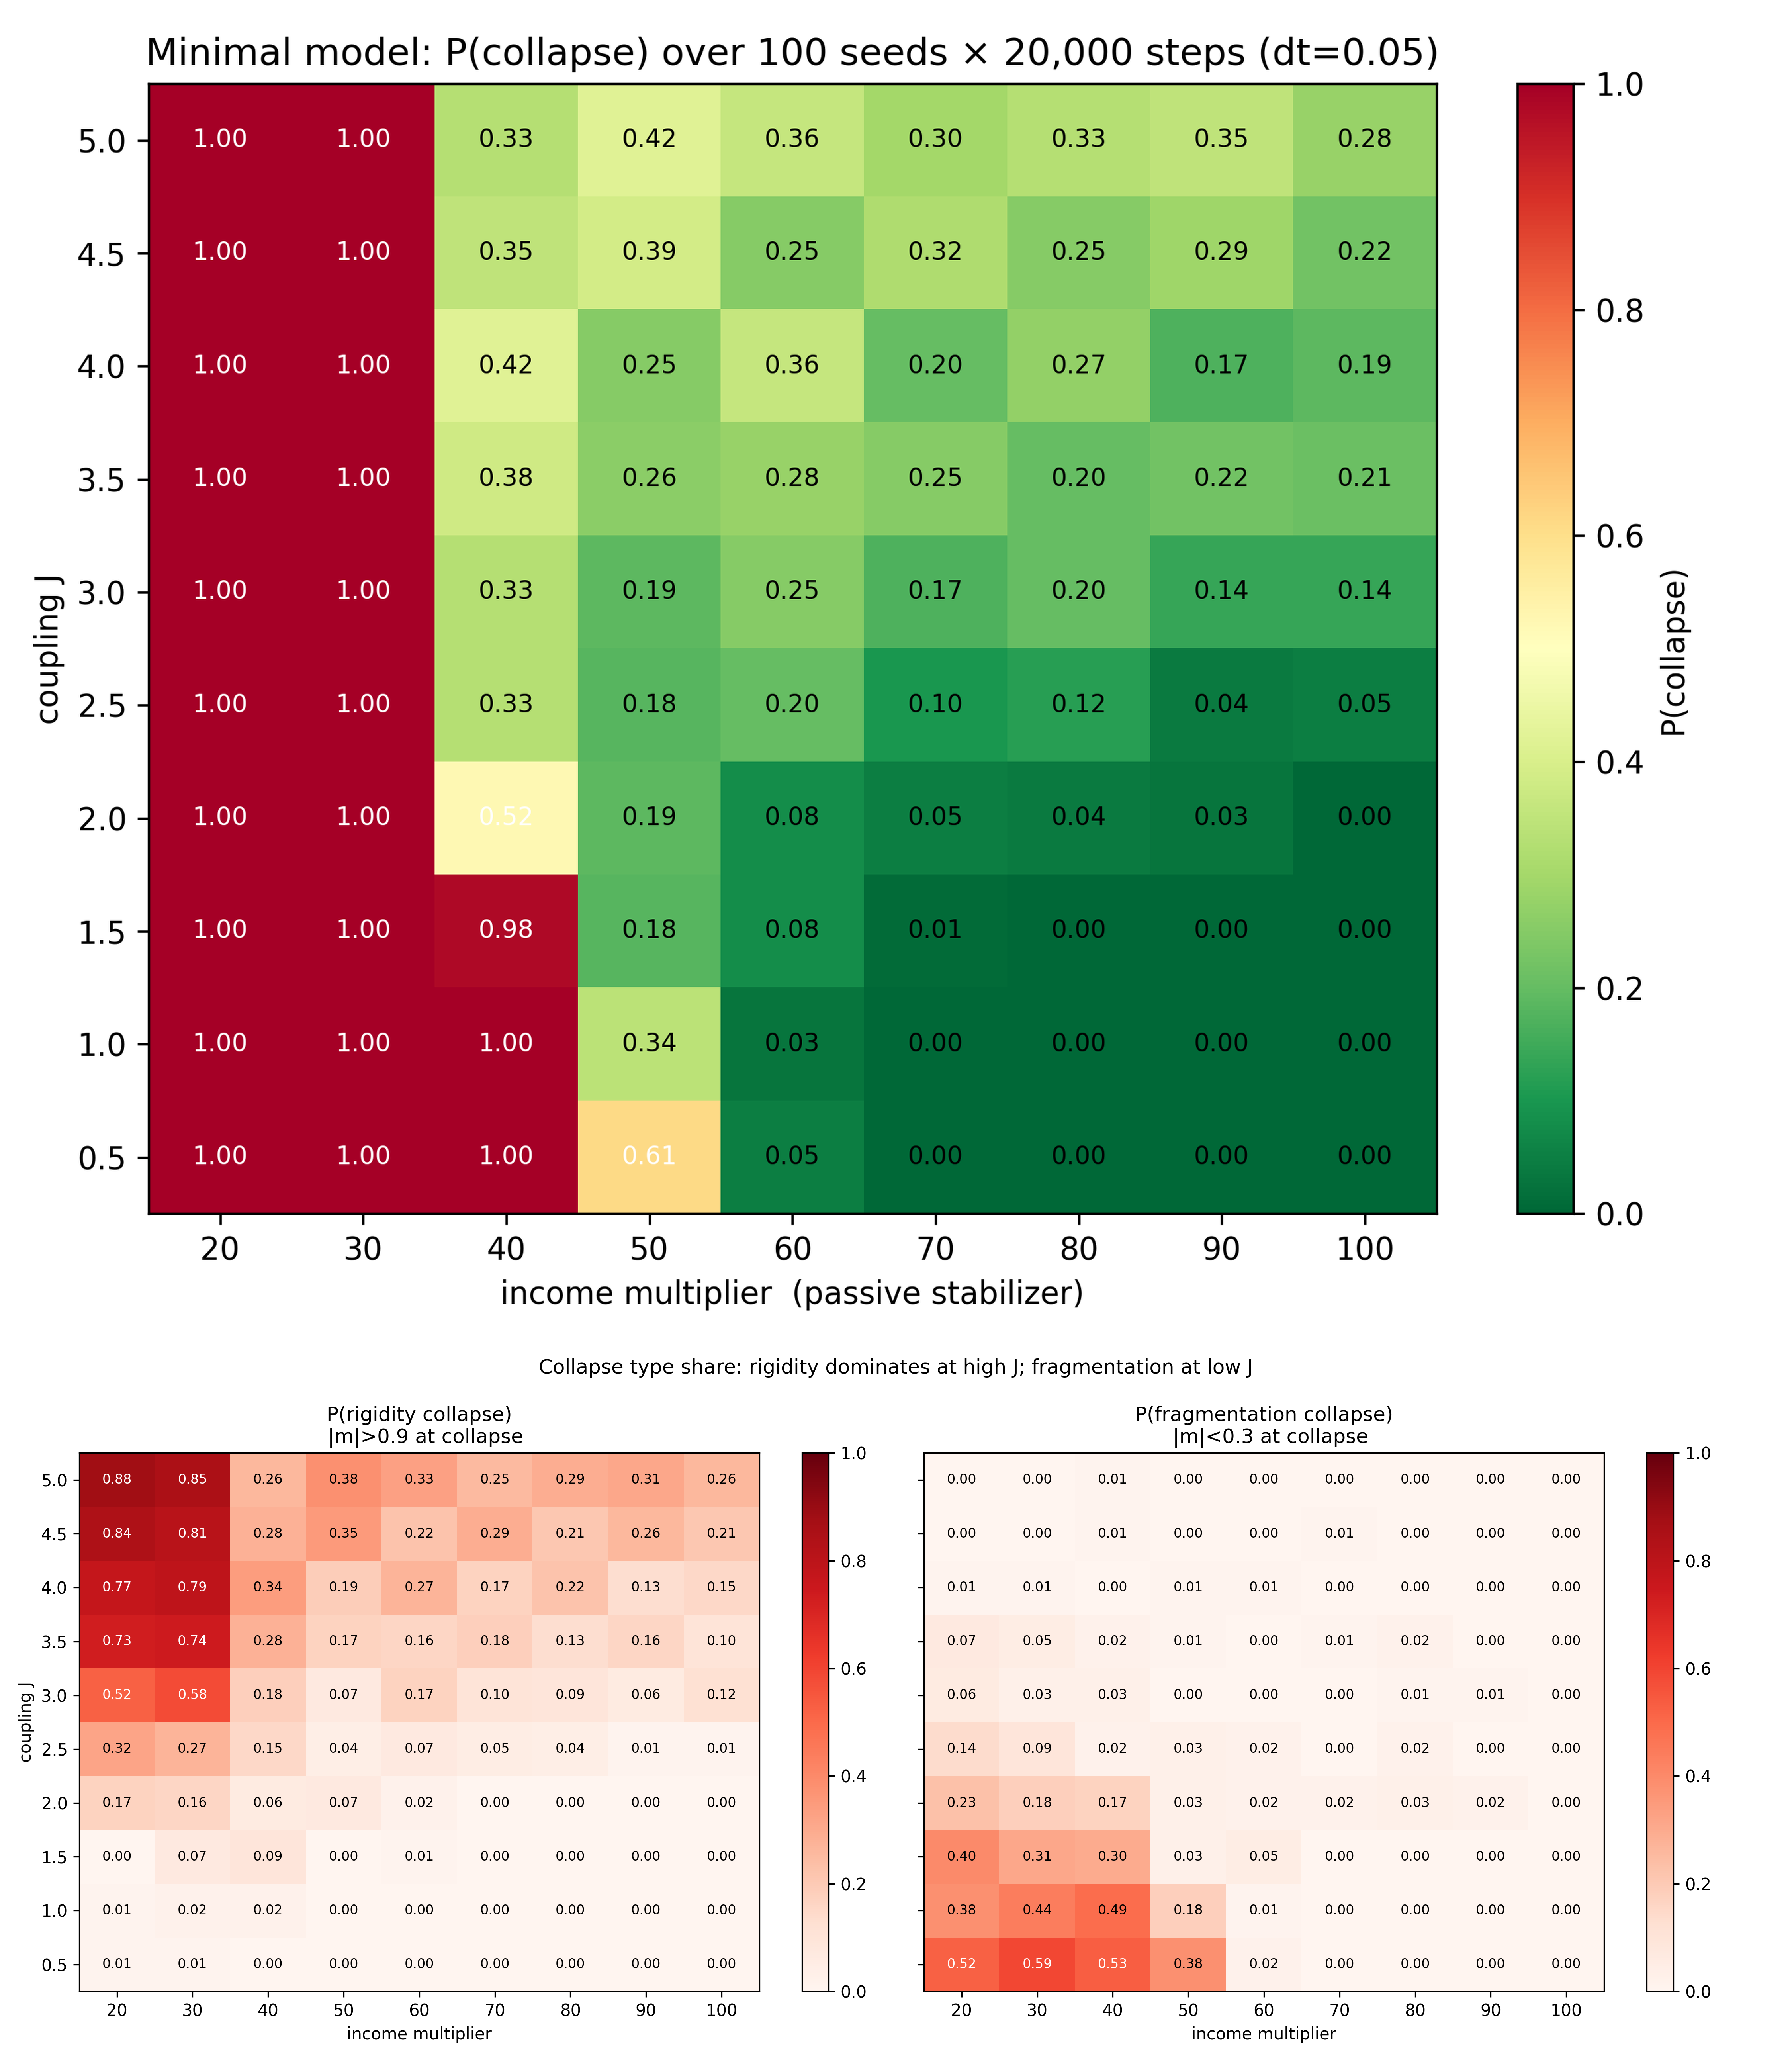
\includegraphics[width=0.95\textwidth]{figures/fig1.png}
\caption{\textit{Static asymmetry in the minimal model.} P(collapse) heatmap over the (\emph{J}, \emph{μ}) grid (upper panel), with cell-level collapse-type composition (lower panels: rigidity share, fragmentation share). 9,000 runs at d\emph{t} = 0.05; 100 seeds per cell. Fragmentation occupies the low-\emph{J}, low-\emph{μ} corner and is fully cured by raising \emph{μ}; rigidity dominates the high-\emph{J} band at every \emph{μ} and saturates above zero (residual P(collapse) = 0.23 at \emph{μ} = 100, 90\% rigidity-typed).}
\label{fig:fig1}
\end{figure*}



\begin{figure*}[!htbp]
\centering
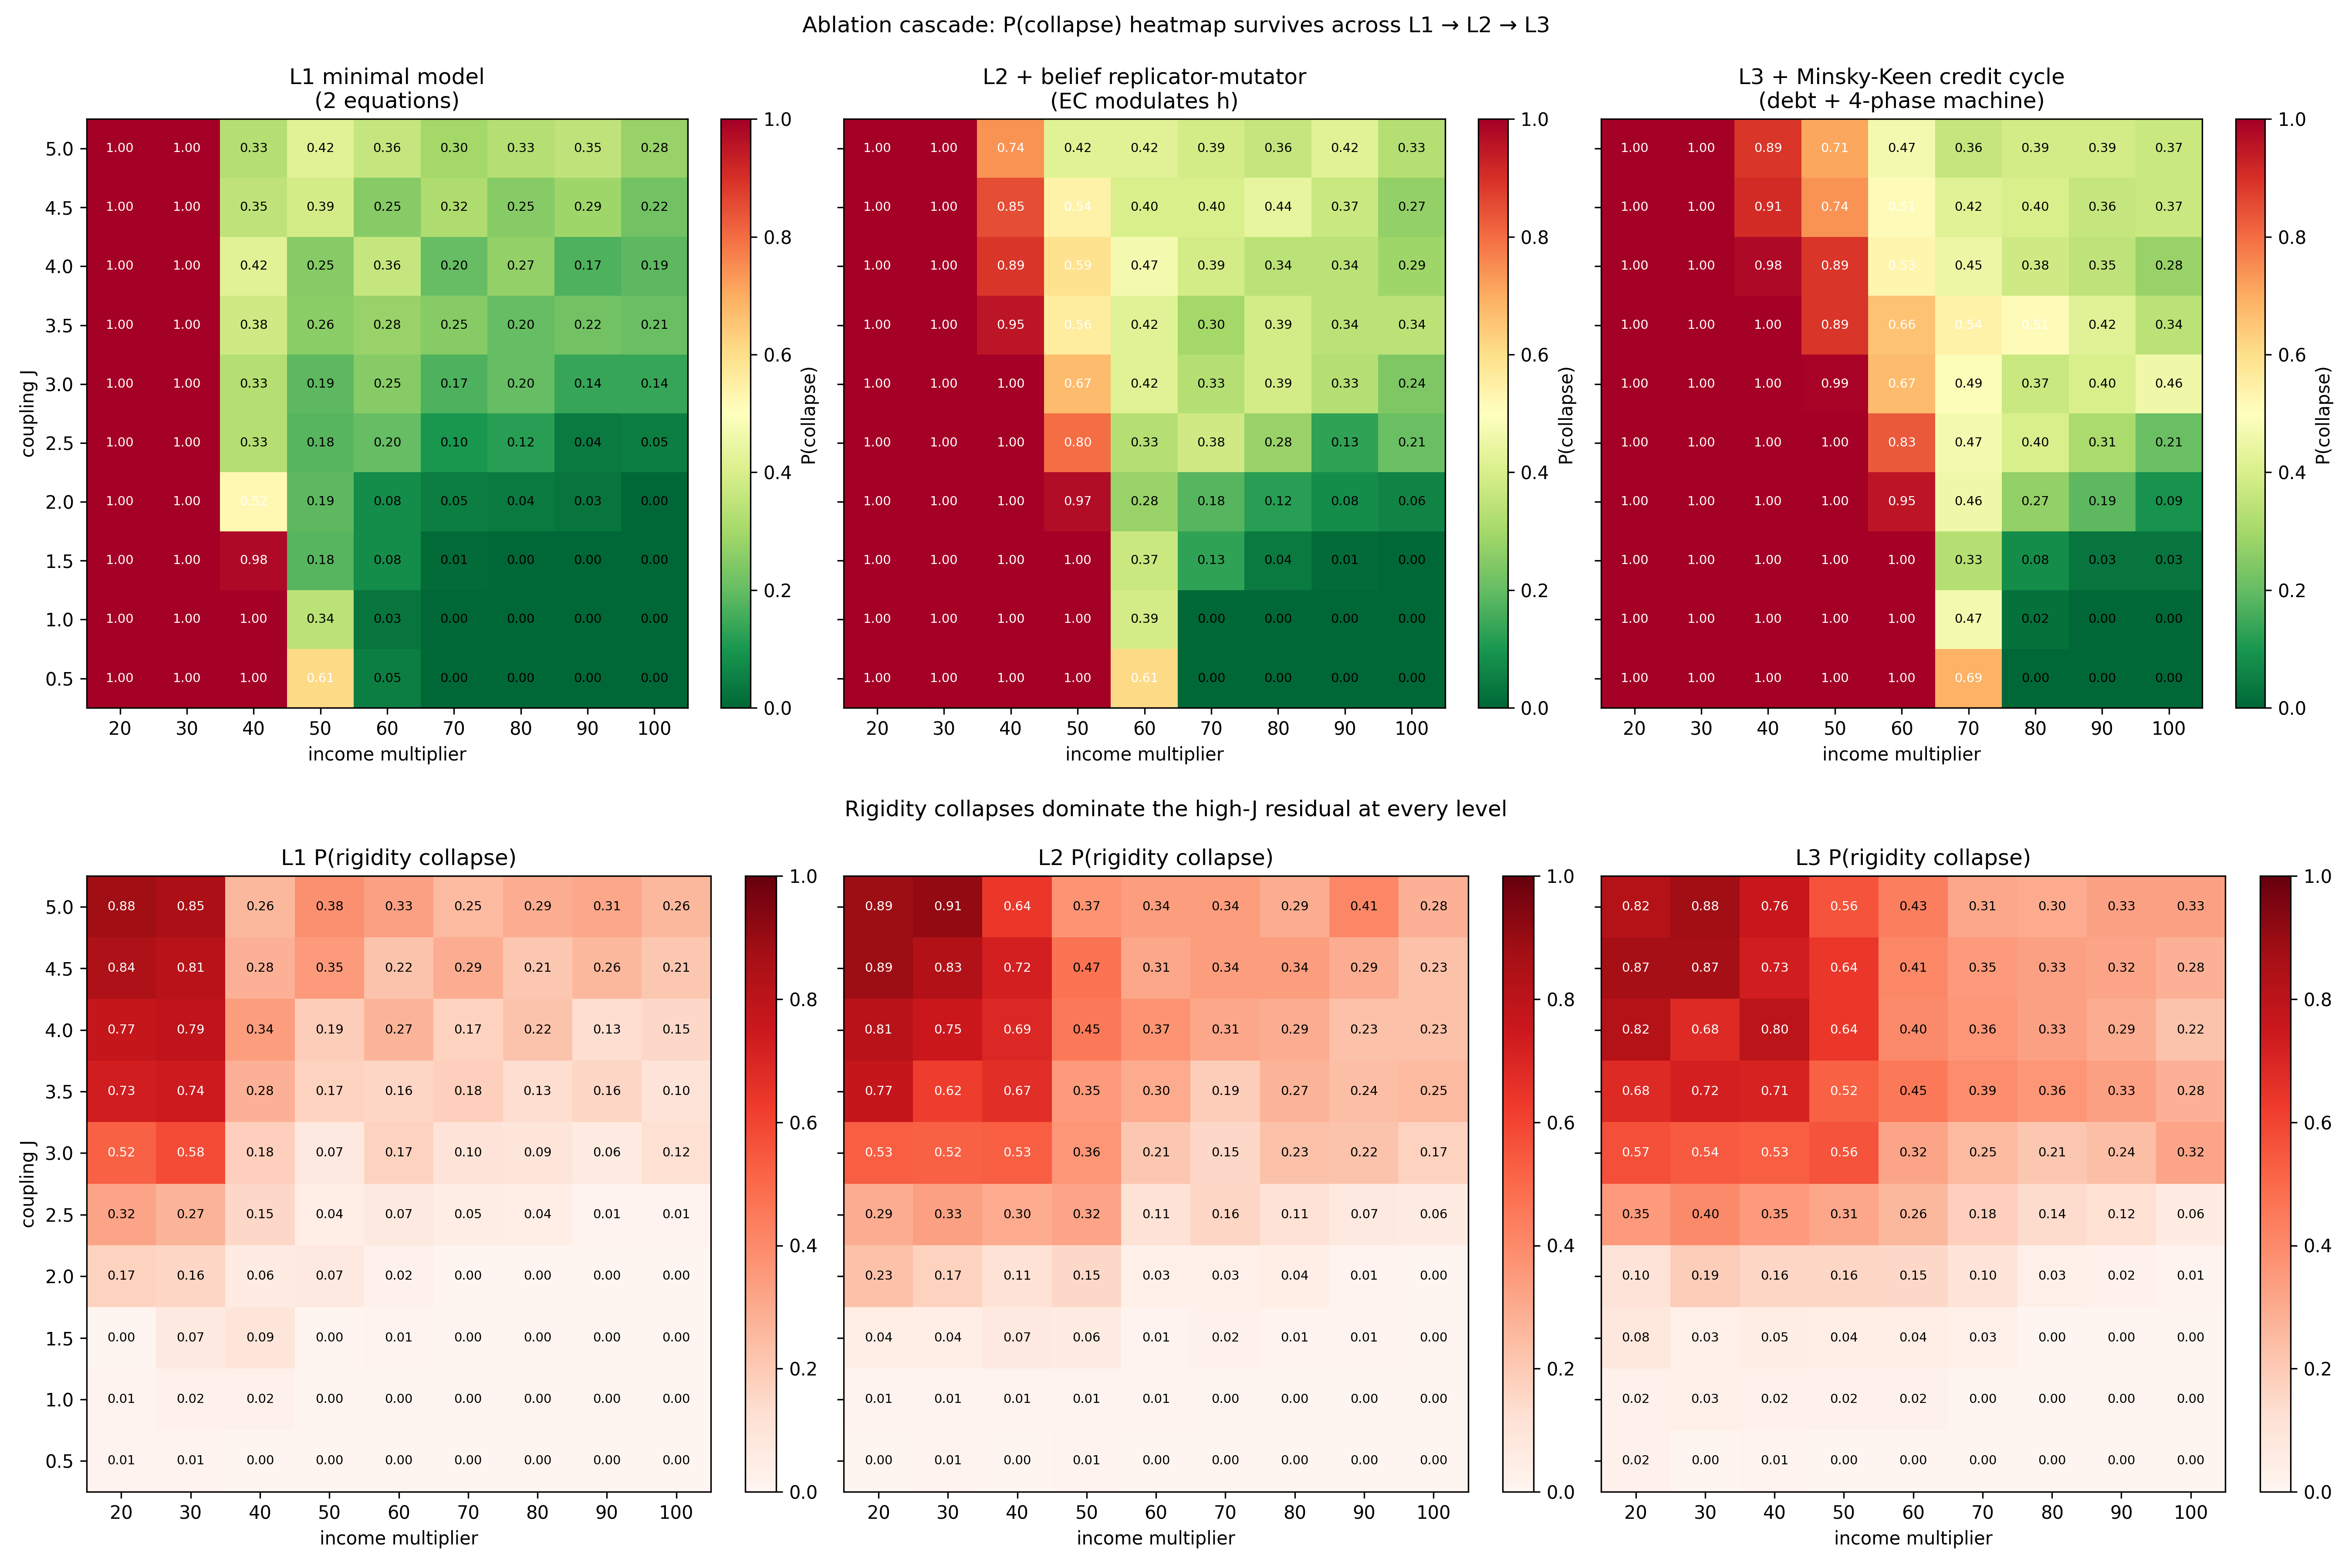
\includegraphics[width=0.95\textwidth]{figures/fig2.png}
\caption{\textit{Ablation cascade L1 → L2 → L3.} Upper panel: P(collapse) heatmap comparison across the three levels of model complexity, on the same (\emph{J}, \emph{μ}) grid as Figure 1. Lower panel: rigidity-share heatmaps for the same three levels. Adding belief dynamics (L2) and credit-cycle dynamics (L3) monotonically \emph{worsens} the high-\emph{J} residual collapse rate (23\% → 30\% → 34\% at \emph{μ} = 100), while preserving rigidity dominance of the residual at every level (90\%, 83\%, 81\%).}
\label{fig:fig2}
\end{figure*}



\begin{figure*}[!htbp]
\centering
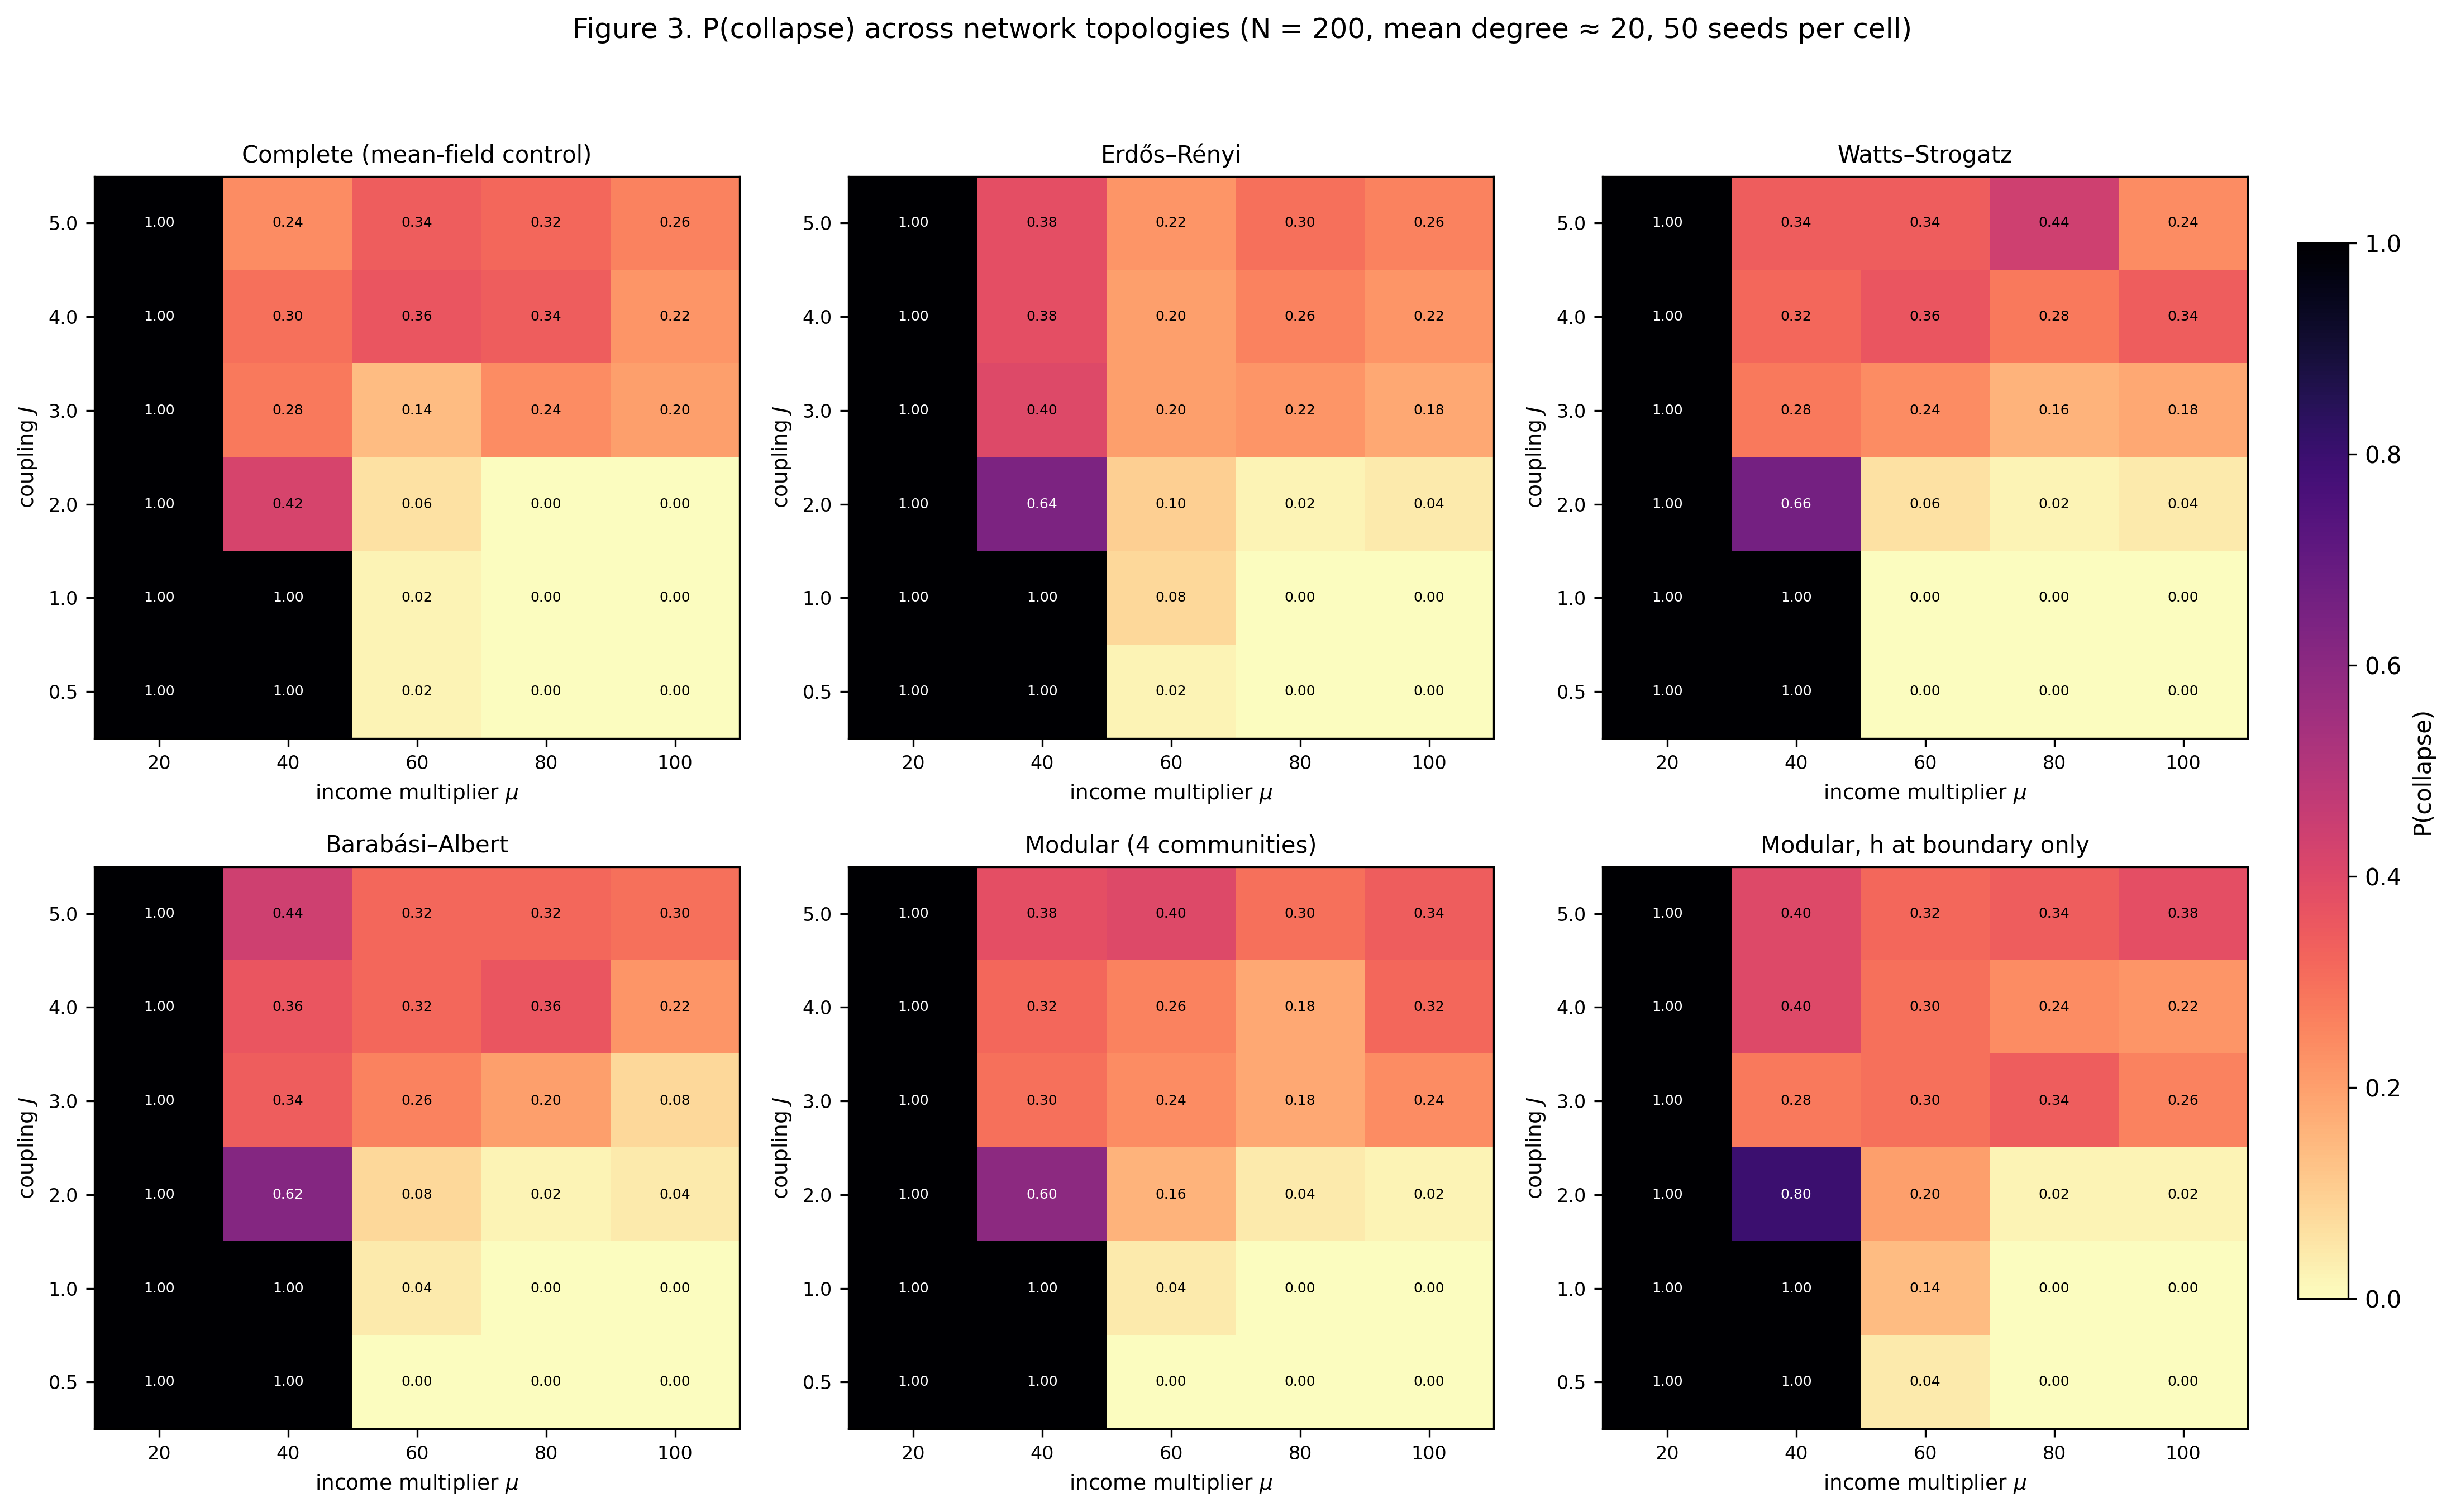
\includegraphics[width=0.95\textwidth]{figures/fig3.png}
\caption{\textit{Network robustness of the h/J² scaling.} P(collapse) heatmaps over the (\emph{J}, \emph{μ}) grid for six network topologies with N = 200 agents: complete graph (mean-field control), Erdős--Rényi, Watts--Strogatz, Barabási--Albert, planted-partition modular (4 communities), and modular with passive stabilizer at community boundaries only. The high-\emph{J} residual survives on every topology. The 50-seed sweep spans 0.24--0.38 across topologies; a 100-seed re-run at the headline cell (\emph{J} = 5, \emph{μ} = 100; SI §S9) shows all six topologies converge to P(collapse) ∈ {[}0.33, 0.37{]}, with no pair separated above one standard error. No tested topology --- including modular and boundary-localized stabilization --- rescues the mean-field residual. 50 seeds per cell for the full grid; d\emph{t} = 0.05.}
\label{fig:fig3}
\end{figure*}



\begin{figure*}[!htbp]
\centering
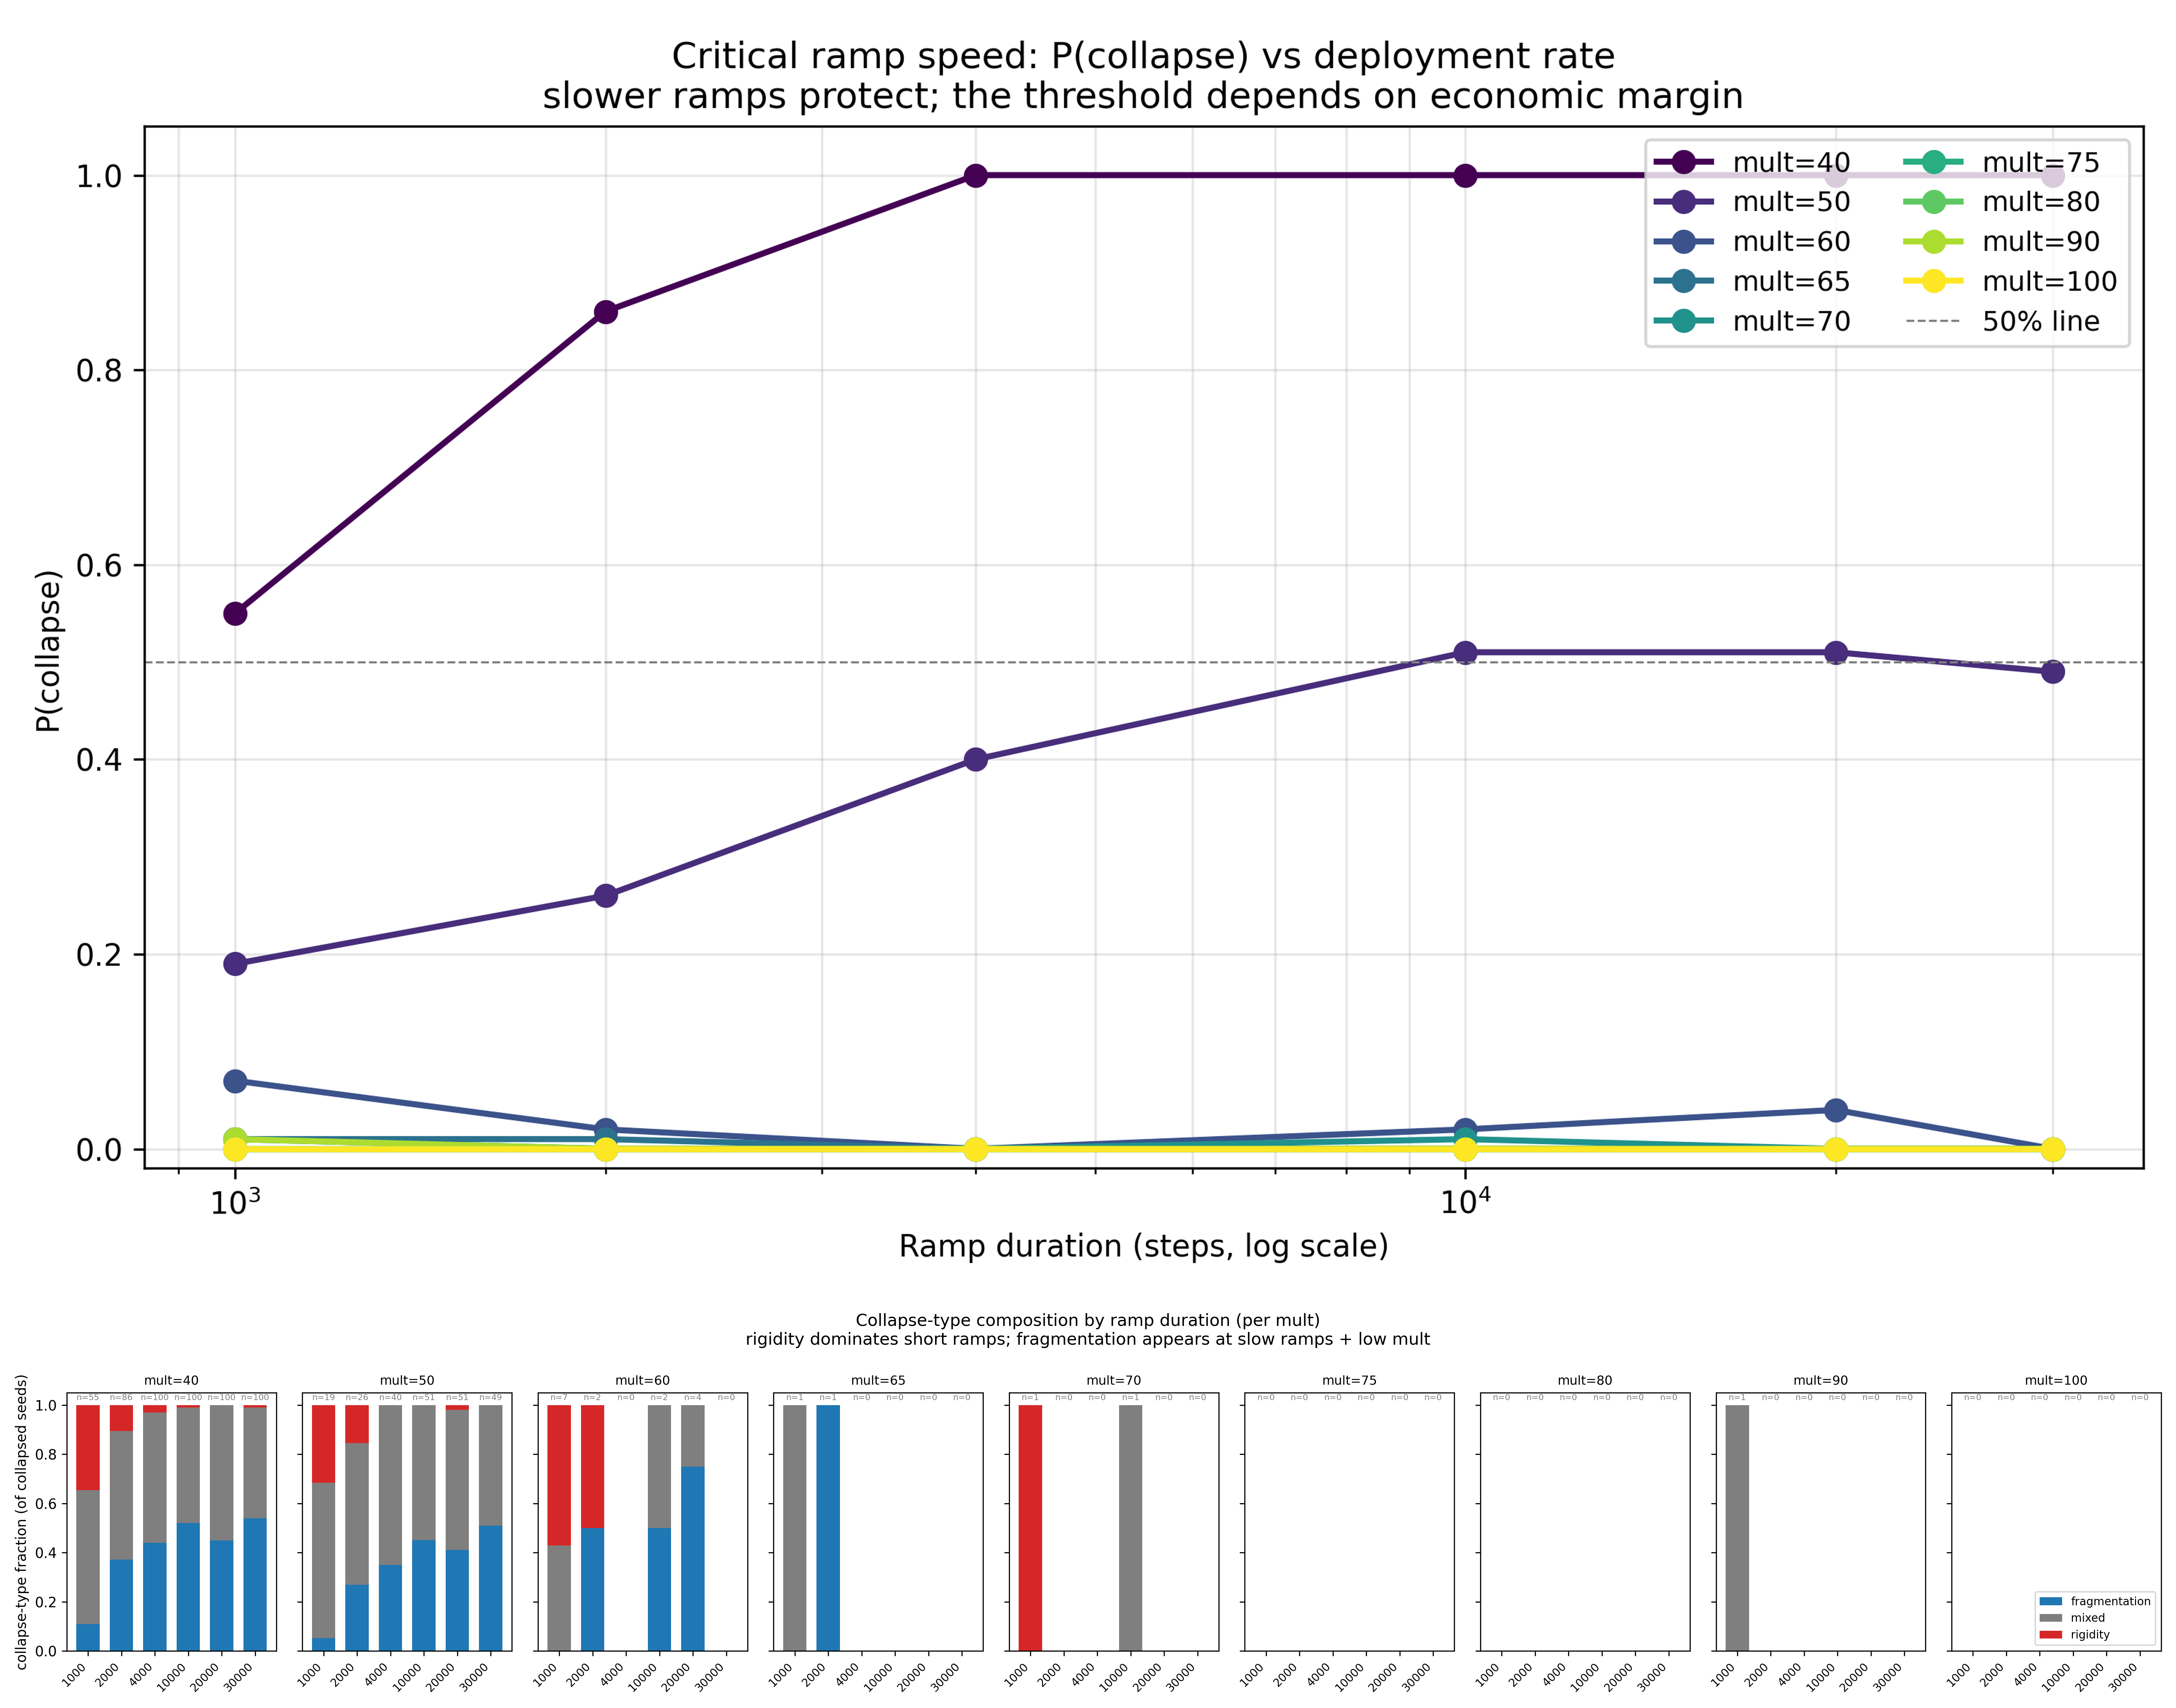
\includegraphics[width=0.95\textwidth]{figures/fig4.png}
\caption{\textit{Critical ramp speed.} Upper panel: P(collapse) as a function of ramp duration (log scale), one curve per economic margin \emph{μ}. Three regimes are visible: resilient (\emph{μ} ≥ 60, ≤ 7\% at every ramp), critical (\emph{μ} = 50, monotonically increasing in ramp duration; 50\% threshold ≈ 9,200 steps), unviable (\emph{μ} ≤ 40, saturated at 1.00 beyond ramp ≈ 4,000 steps). Lower panel: collapse-type composition (rigidity, fragmentation, mixed) versus ramp duration, broken out by \emph{μ}. The dominant failure mode swaps from rigidity (fast ramps) to fragmentation (slow ramps) at low margins. 5,400 runs at d\emph{t} = 0.05.}
\label{fig:fig4}
\end{figure*}



\begin{figure*}[!htbp]
\centering
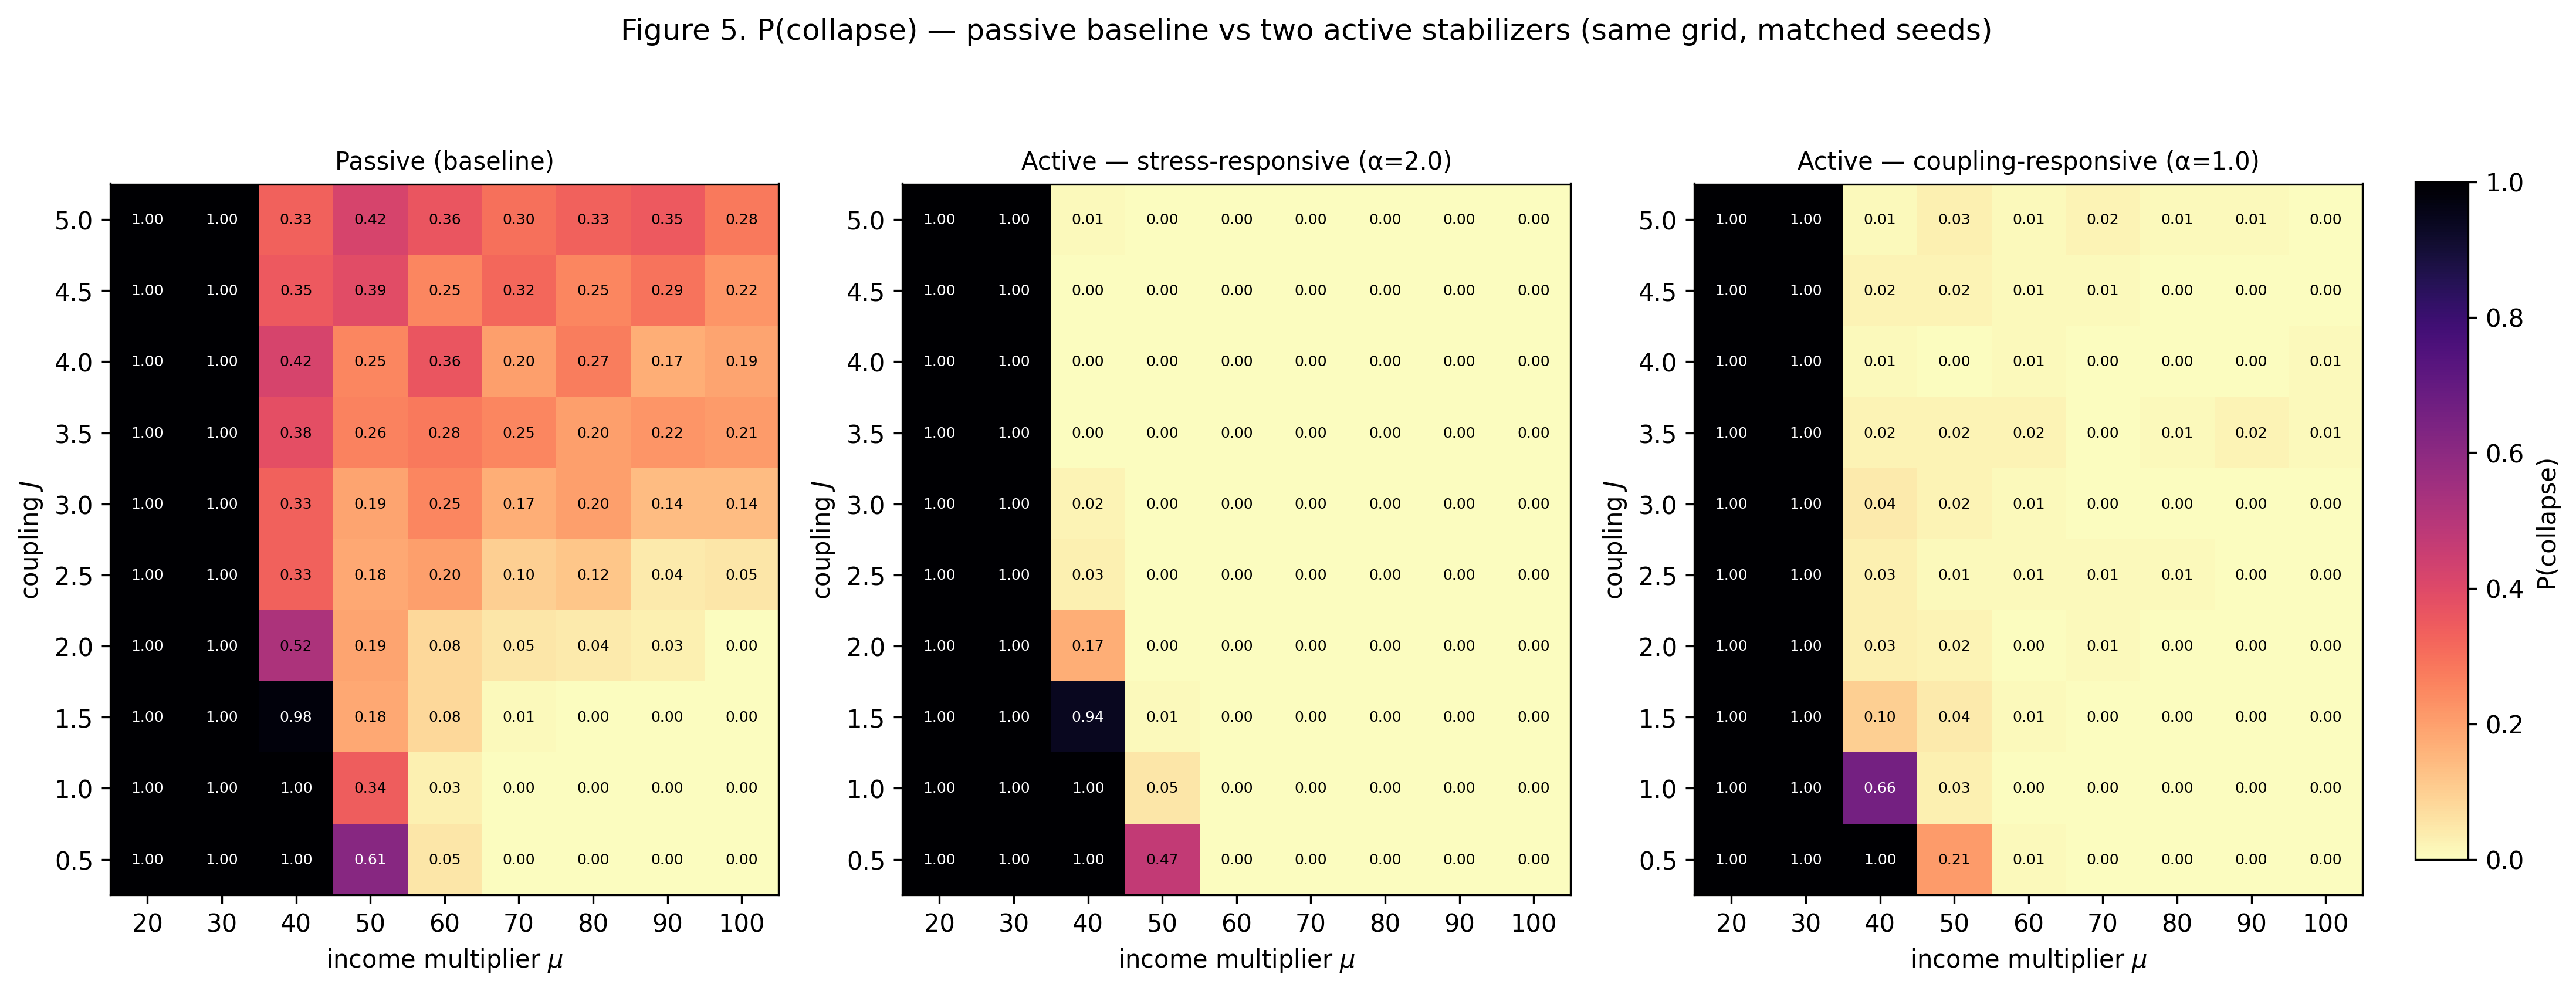
\includegraphics[width=0.95\textwidth]{figures/fig5.png}
\caption{\textit{Active vs.~passive stabilizer effectiveness.} P(collapse) heatmaps over the (\emph{J}, \emph{μ}) grid for three conditions with matched seeds: passive baseline (left), stress-responsive active stabilizer with α = 2.0 (center), and coupling-responsive active stabilizer with α = 1.0 (right). The passive baseline reproduces the high-\emph{J} residual (band-mean 0.23 at \emph{μ} = 100, 90\% rigidity-typed); both active variants eliminate it entirely (P(collapse) = 0.00 across \emph{J} ≥ 4.0 at \emph{μ} = 100). 9,000 runs per condition at d\emph{t} = 0.05.}
\label{fig:fig5}
\end{figure*}



\begin{figure*}[!htbp]
\centering
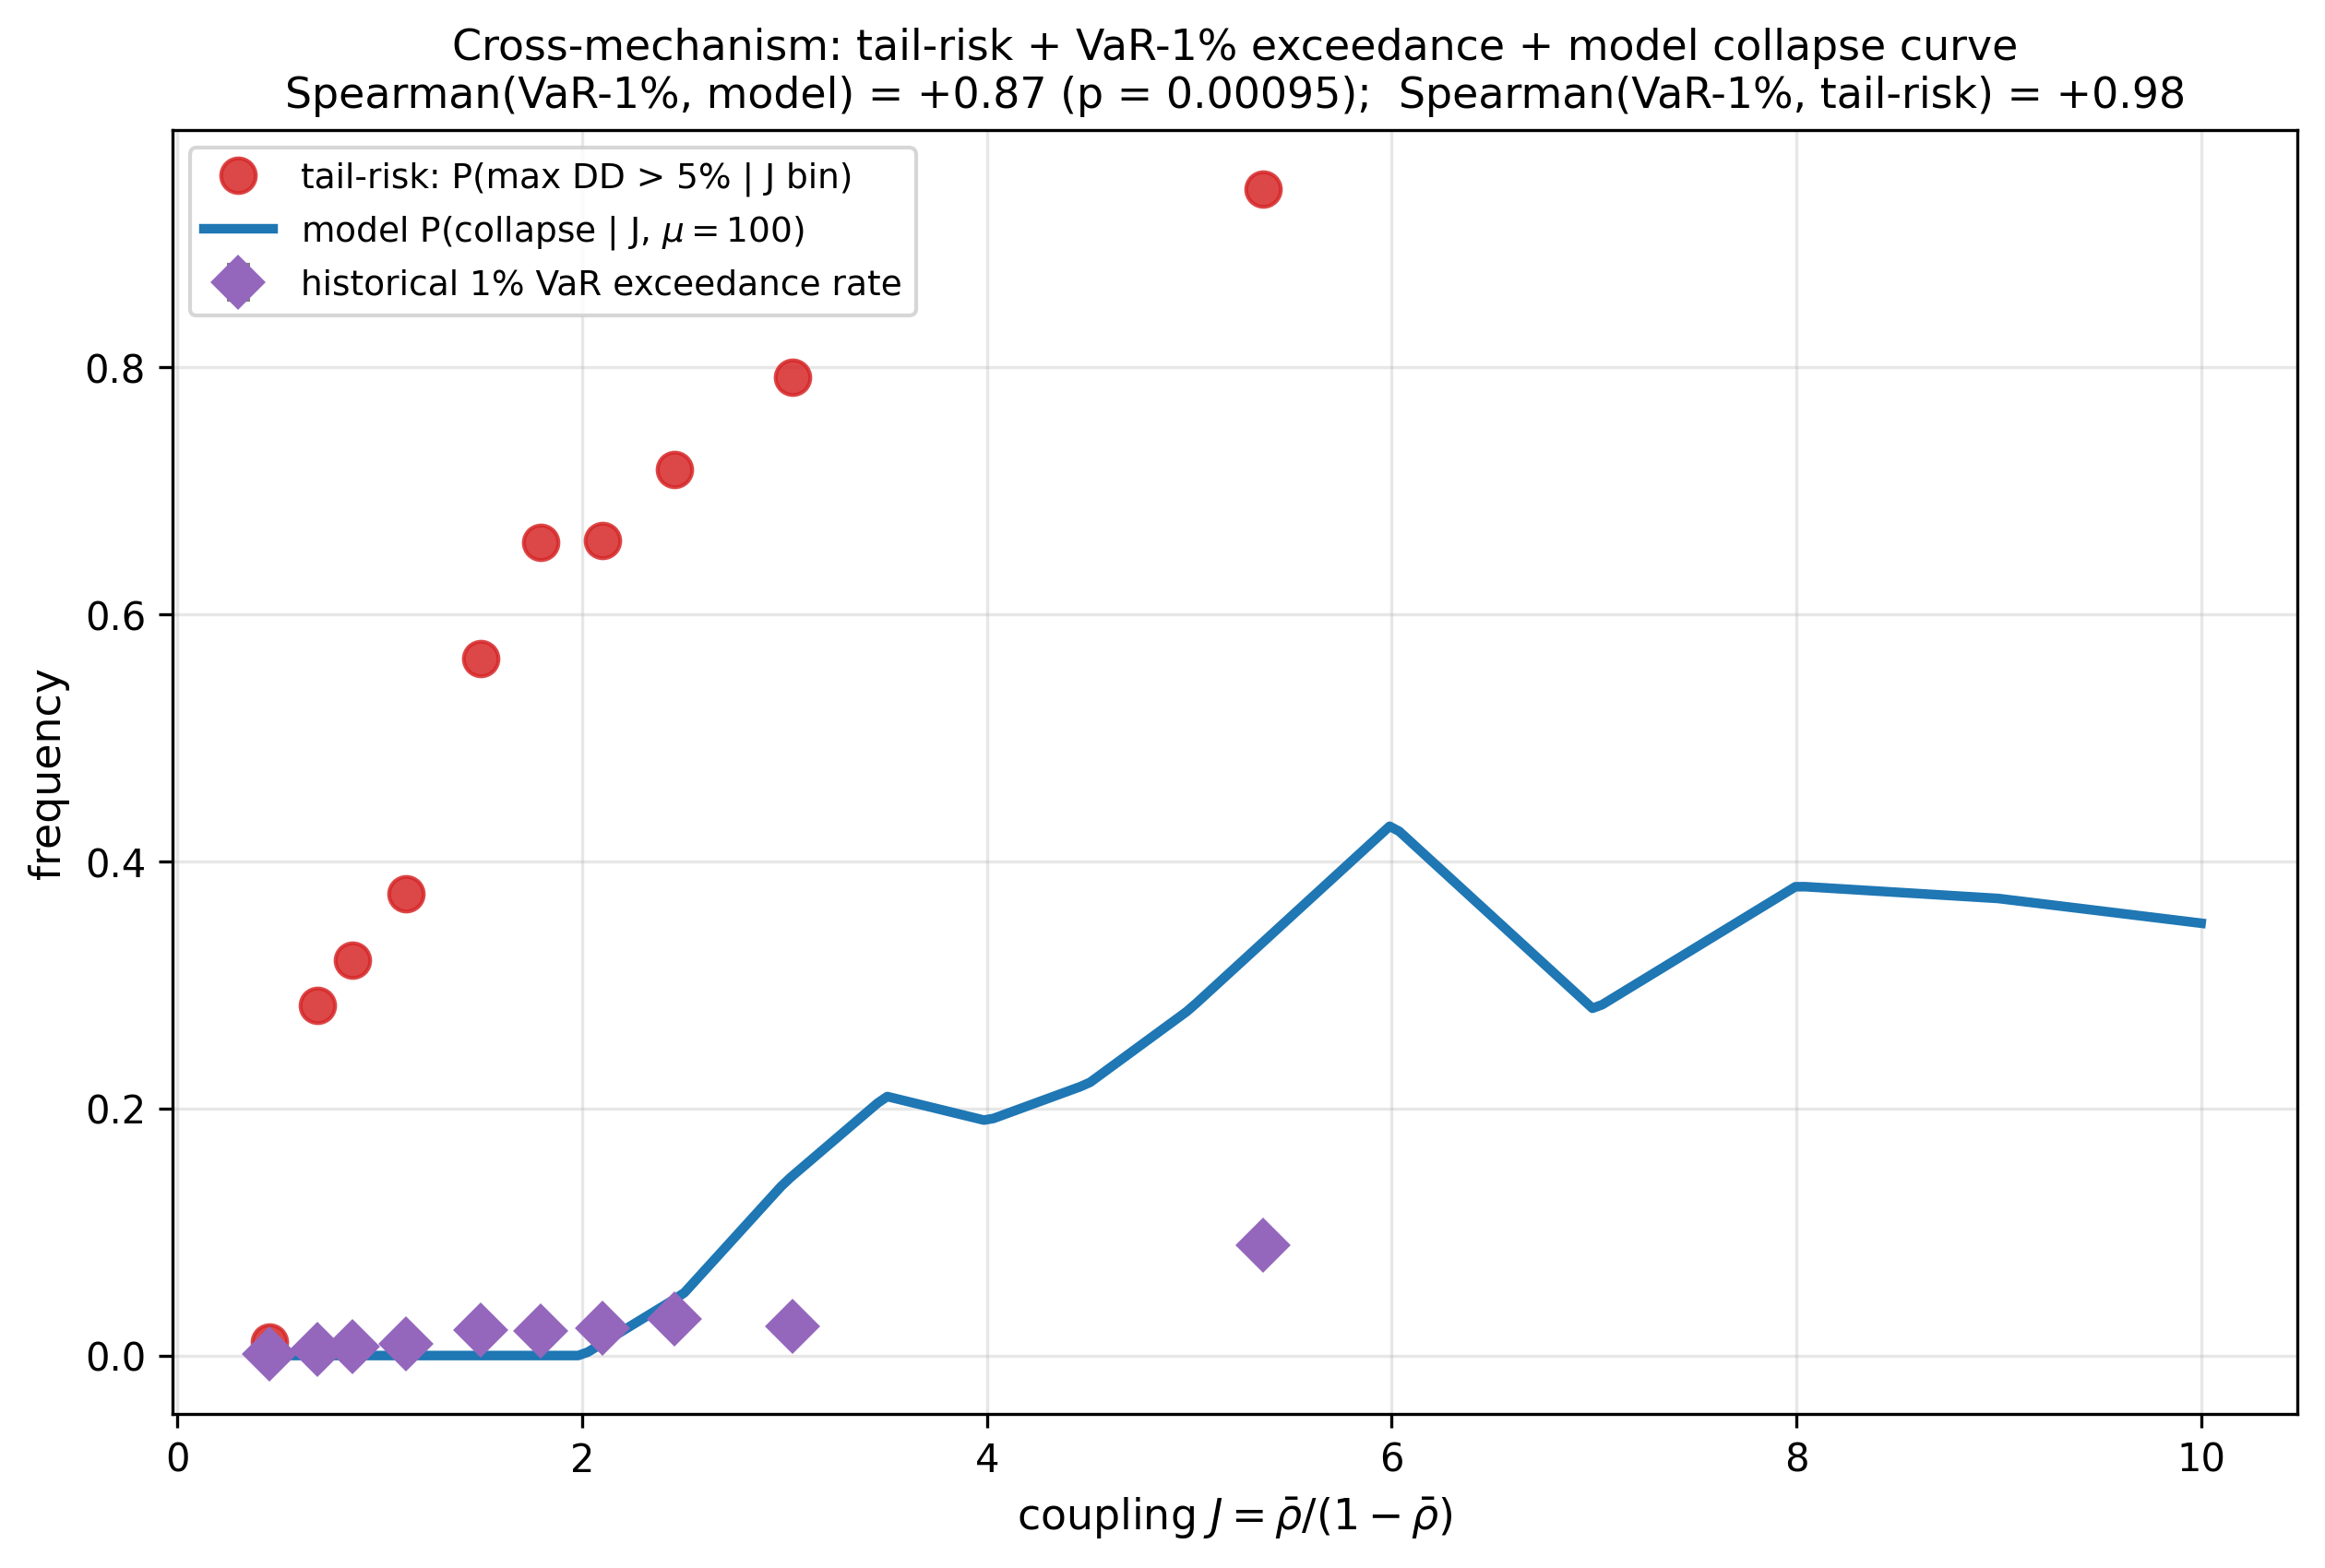
\includegraphics[width=0.95\textwidth]{figures/fig6.png}
\caption{\textit{Mechanism test: tail-risk frequency and VaR exceedance vs.~coupling.} Empirical P(max drawdown \textgreater{} 5\%) (red points) and historical 1\% VaR exceedance rate (purple diamonds) across coupling deciles, overlaid with the model's P(collapse \textbar{} \emph{J}, \emph{μ} = 100) curve (blue line). All three track the same coupling axis. Spearman ρ = +0.81 (tail-risk vs.~model) and +0.87 (VaR-1\% vs.~model); cross-mechanism ρ = +0.98 between the two empirical curves. The model's curve is steeper in log-\emph{J} than the empirical data (log-log slope 2.51 vs.~1.45 at the 5\% threshold), reflecting the mean-field branch-selection mechanism's overstatement of the rate at which passive-stabilizer effectiveness decays at intermediate coupling --- the direction and rank order are robust, the absolute slope is model-specific. 5,414 windows (tail risk), 4,910 windows (VaR, shorter due to 252-day lookback).}
\label{fig:fig6}
\end{figure*}



\begin{figure*}[!htbp]
\centering
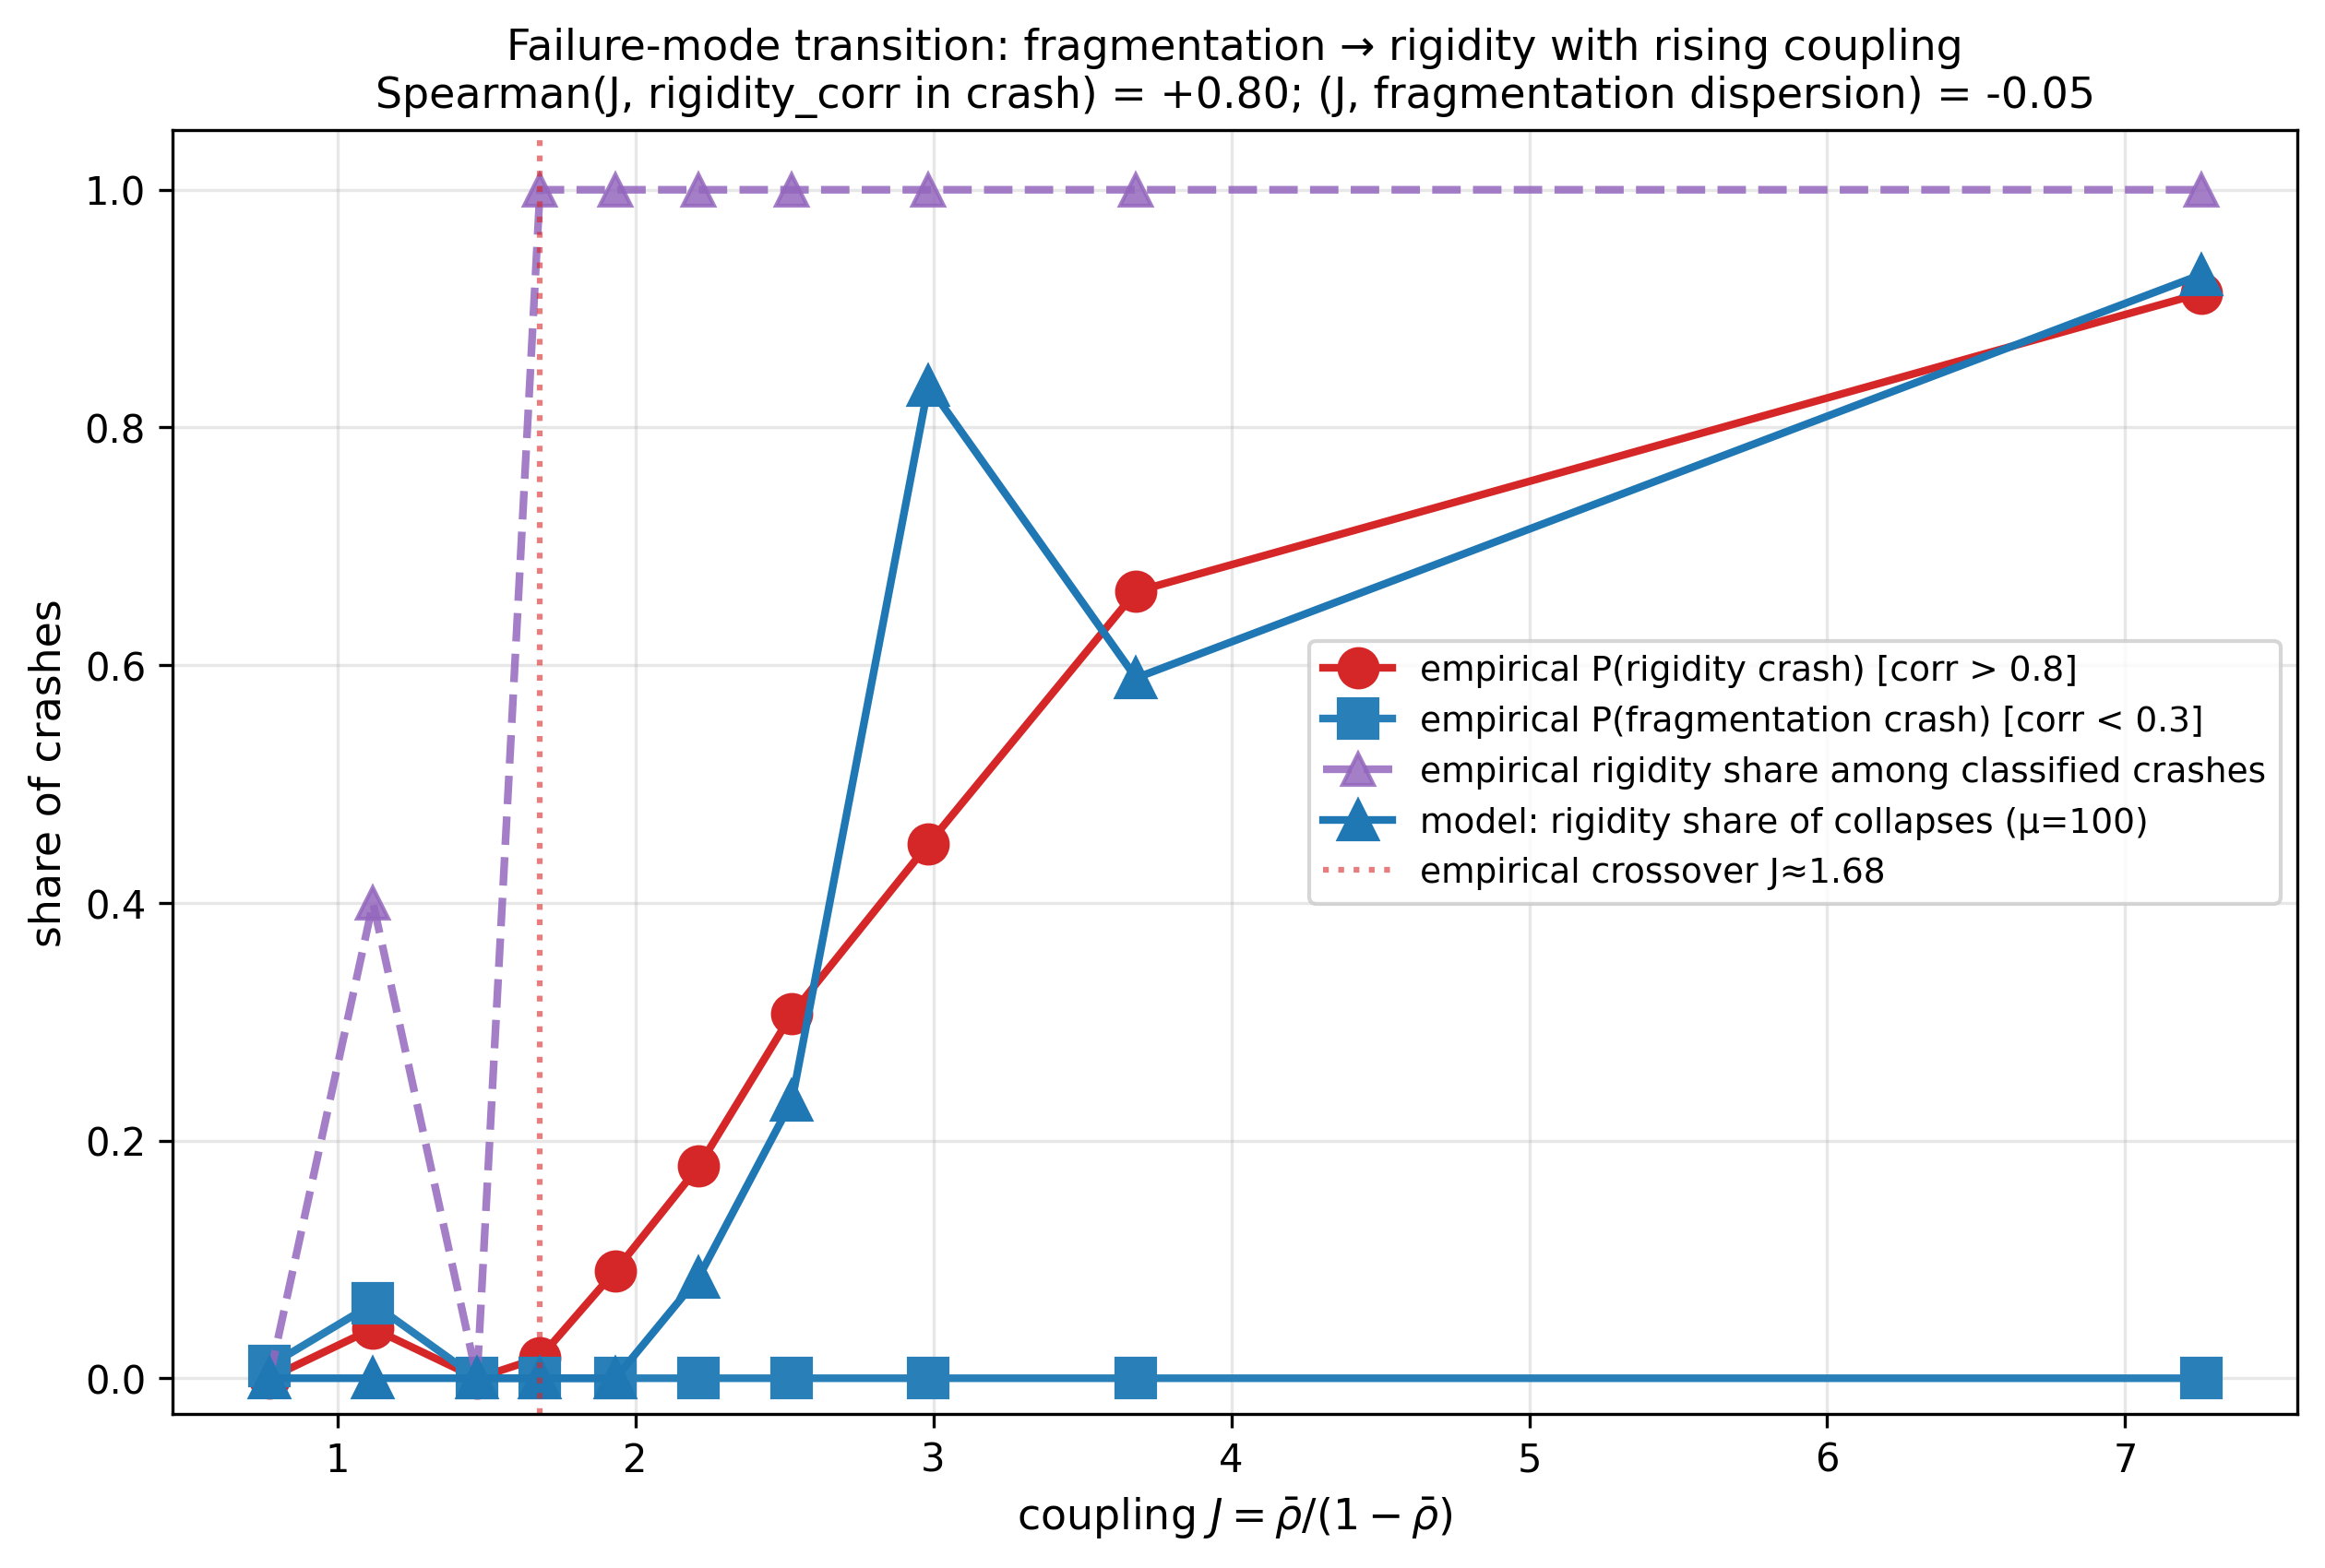
\includegraphics[width=0.95\textwidth]{figures/fig7.png}
\caption{\textit{Failure-mode transition: rigidity vs.~fragmentation.} Empirical share of rigidity-typed crashes per decile (red circles; crash-window mean pairwise correlation \textgreater{} 0.8) and share of fragmentation-typed crashes (blue squares; correlation \textless{} 0.3), together with the rigidity share among classified crashes (purple triangles, dashed) and the model's predicted rigidity-share-of- collapses curve (blue triangles, \emph{μ} = 100). The mean within-crash pairwise correlation (not plotted, given in the per-decile table) rises monotonically from 0.50 (lowest coupling) to 0.88 (highest); the empirical rigidity-share crossover (\emph{J} ≈ 1.7) is within a factor of 1.8 of the model's predicted crossover (\emph{J} ≈ 3.0). Spearman ρ(\emph{J}-decile, mean within-crash correlation) = +1.00 (perfect monotone; exact permutation \emph{p} = 2/10! ≈ 5.5 × 10⁻⁷); Spearman correlation between empirical within-crash correlation and model rigidity-share = +0.92 (\emph{p} = 1.3 × 10⁻⁴). 2,869 crash windows (max drawdown \textgreater{} 5\% within the 60-day window), \textasciitilde287 per decile.}
\label{fig:fig7}
\end{figure*}



\begin{figure*}[!htbp]
\centering
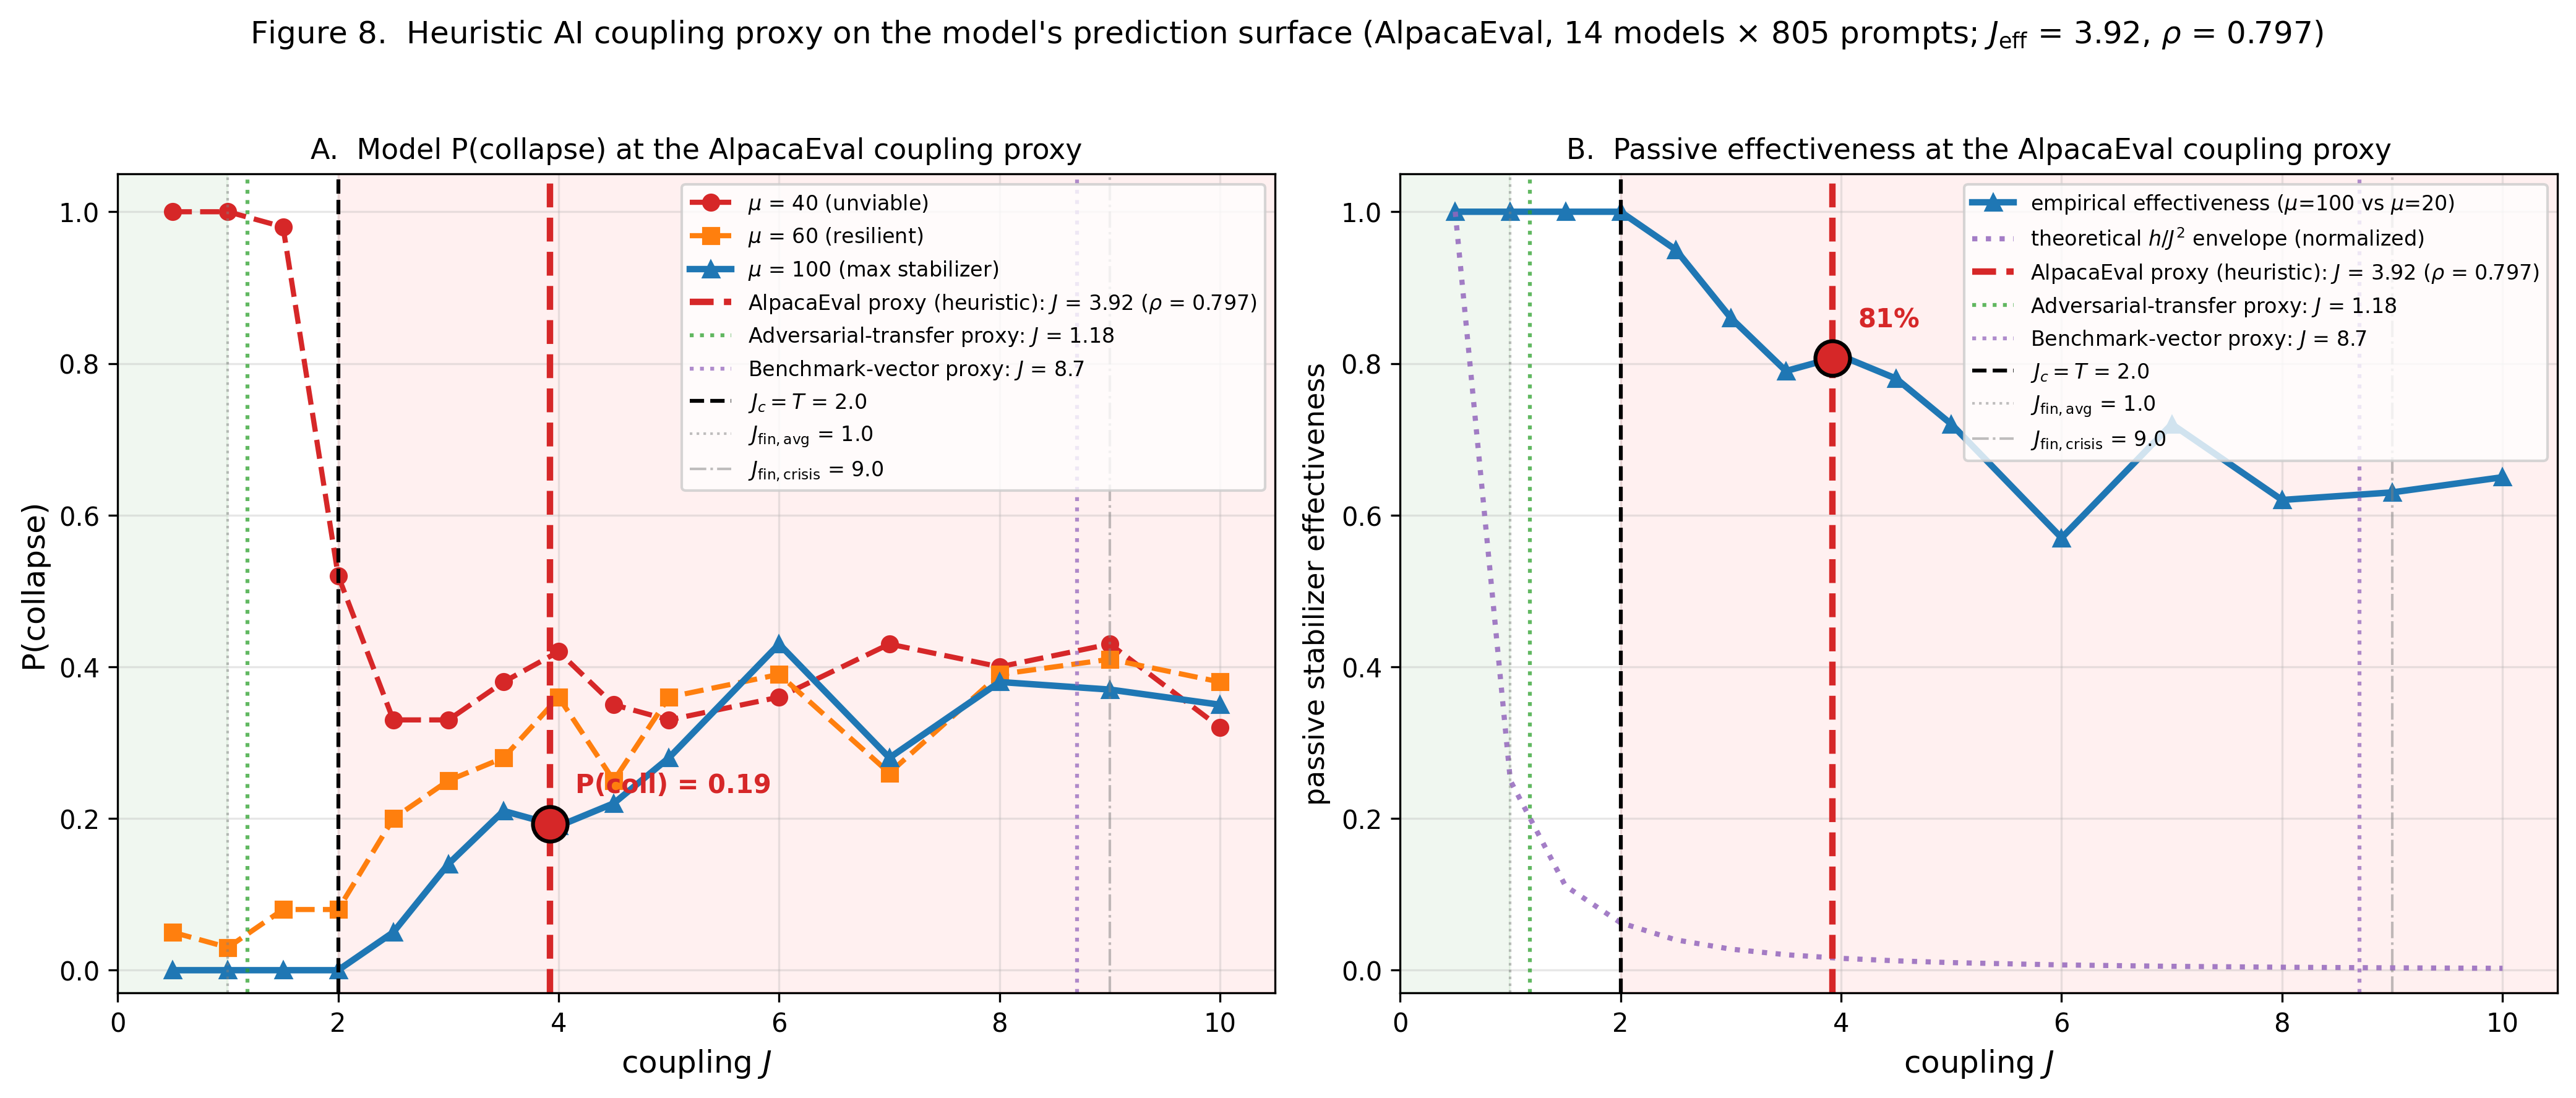
\includegraphics[width=0.95\textwidth]{figures/fig8.png}
\caption{\textit{Heuristic AI coupling proxy on the model's prediction surface.} Panel A: P(collapse) versus coupling \emph{J} for three economic margins (\emph{μ} = 40, 60, 100). The dashed red vertical line marks the AlpacaEval output-similarity proxy (ρ = 0.797, \emph{J}ₑff = 3.92; 14 frontier models × 805 prompts; heuristic, not calibrated). Dotted lines show the two earlier proxy estimates: adversarial-attack transferability (\emph{J} ≈ 1.2, green) and benchmark-vector correlation (\emph{J} ≈ 8.7, purple). Black dashed line: critical threshold \emph{J}ᶜ = \emph{T} = 2. Financial reference lines at \emph{J} = 1.0 (average) and \emph{J} = 9.0 (crisis). Panel B: passive stabilizer effectiveness (1 − P(\emph{J}, \emph{μ} = 100)/P(\emph{J}, \emph{μ} = 20)) versus \emph{J} with the same overlays, plus the theoretical \emph{h}/\emph{J}² envelope (purple dotted, normalized). At the proxy-located coupling, the model's P(collapse) surface gives 0.19 with passive effectiveness 81\% at \emph{μ} = 100; this is the model's reading of the proxy, not a calibrated AI prediction (see ``AI coupling'' subsection caveats). Sweep extended to \emph{J} = 10 (Methods).}
\label{fig:fig8}
\end{figure*}



\bibliographystyle{unsrtnat}
\bibliography{references}

\appendix
\renewcommand{\thesection}{S\arabic{section}}
\renewcommand{\thesubsection}{S\arabic{section}.\arabic{subsection}}
\renewcommand{\thefigure}{S\arabic{figure}}
\setcounter{figure}{0}
\setcounter{section}{0}

\section*{Supplementary Information}

\textbf{Paper:} \emph{Why Fixed Protections Fail Under Rising Coordination: A Structural Failure-Mode Transition in Coupled Systems}

This document supplies the technical material referenced in the main text. §S1 fully specifies the L2, L3, and L4 dynamical systems used in the ablation cascade. §S2 gives the \emph{a priori} derivation of the \emph{h}/\emph{J}² scaling of Theorem 1 from the Curie--Weiss free-energy structure. §S3 presents Figure S1 (the L0 mean-field validation). §S4 documents the full convergence test that motivates the d\emph{t} = 0.05 choice in Methods. §S5 contains sensitivity and robustness analyses (noise prescription, \emph{h}(\emph{W}) form, parameter OAT, alternative model classes, and a cryptocurrency cross-domain extension). §S6 establishes the formal correspondence between the diversification identity (main-text Equation 3) and the Theorem 1 scaling. §S7 compares this work with the five closest existing frameworks referenced in the main text. §S8 details the AI coupling measurements reported in the Discussion. §S9 provides implementation details for the network agent-based model. §S10 reports tail-risk and VaR exceedance details, including out-of-sample temporal prediction, nonlinearity characterization, the fragmentation-to-rigidity failure-mode transition, and the Fed active-stabilizer empirical fit. §S11 contains supplementary Figure S2 (diversification structural form, supporting the main-text ``Empirical setting'' subsection), Figure S3 (the 14 × 14 direct AI coupling heatmap), Figure S4 (sensitivity sweep across noise prescription and \emph{h}(\emph{W}) form, supporting §S5.1), Figure S5 (alternative-model-class robustness, supporting §S5.3 --- the asymmetry is not Curie--Weiss-specific), and Figure S6 (crypto cross-domain extension, supporting §S5.4).

\begin{center}\rule{0.5\linewidth}{0.5pt}\end{center}

\section{Full model specifications for the ablation cascade}\label{full-model-specifications-for-the-ablation-cascade}

This section expands the Methods description of Levels 2, 3, and 4 of the ablation cascade with the full dynamical content. Levels 0 and 1 are completely specified in the main text and are not reproduced here.

\subsection{Level 2 --- minimal model + replicator--mutator beliefs}\label{level-2-minimal-model-replicatormutator-beliefs}

Level 2 augments the L1 dynamics with a population of \emph{K} = 6 belief types competing inside each simulated polity. Let \emph{f}ₖ(\emph{t}) denote the fraction of agents holding belief type \emph{k} ∈ \{0, \ldots, \emph{K} -- 1\}, with ∑ₖ\emph{f}ₖ = 1. Each belief type sits at a fixed location \emph{b}ₖ ∈ {[}--1, 1{]} on a one-dimensional opinion axis,

\[
b_k = \frac{2k - (K-1)}{K-1}, \qquad k = 0, \ldots, K-1,
\]

so that the belief axis spans the same range as the coordination order parameter \emph{m}. The replicator-mutator dynamics evolve \emph{f}ₖ between simulation steps according to

\[
f_k(t + \Delta t) = (1 - \mu_b)\,\frac{f_k(t)\,W_k(m)}{\langle W \rangle} + \frac{\mu_b}{K},
\]

with mutation rate \emph{μ}ᵦ = 0.01 and \emph{m}-coupled fitness

\[
W_k(m) = \exp(\gamma\,b_k\,m), \qquad \langle W \rangle = \sum_j f_j(t)\,W_j(m).
\]

The fitness coupling \emph{γ} = 1 implies that beliefs aligned with the current sign of \emph{m} are favored. The renormalization against ⟨\emph{W}⟩ keeps ∑ₖ\emph{f}ₖ = 1 to numerical precision; an additional unconditional renormalization by ∑ₖ\emph{f}ₖ at the end of each step absorbs any drift from finite-precision arithmetic.

The epistemic-coherence factor is the normalized Shannon entropy of the belief distribution,

\[
\mathrm{EC}(t) = \frac{-\sum_k f_k(t) \ln f_k(t)}{\ln K} \in [0, 1],
\]

with EC = 1 indicating uniform belief diversity and EC = 0 indicating complete monoculture. The L2 passive stabilizer field is

\[
h_{\mathrm{eff}}(t) = h(W(t)) \cdot \mathrm{EC}(t),
\]

so the operative restoring force in Equation 1 of the main text is \emph{h}ₑff rather than \emph{h}. All other dynamics --- the SDE for \emph{m}, the wealth equation, and the collapse criteria --- are identical to L1.

Mechanism: at high coupling \emph{J}, the \emph{m}-coupled fitness drives the belief distribution toward whichever single type aligns with the saturated \emph{m}; EC drops toward 1/log \emph{K} ≈ 0.06 in the limit of full monoculture. The passive stabilizer's effective field is then strongly attenuated even though the underlying wealth-driven \emph{h} is intact. At low \emph{J}, \emph{m} never saturates, fitness selection is weak, and EC remains high enough that \emph{h}ₑff ≈ \emph{h}.

\subsection{Level 3 --- L2 + Minsky--Keen credit cycle}\label{level-3-l2-minskykeen-credit-cycle}

Level 3 adds a four-phase credit machine to the L2 dynamics. Each simulated polity carries an aggregate debt state \emph{D}(\emph{t}) and a phase indicator \emph{p}(\emph{t}) ∈ \{Expansion, Euphoria, MinskyMoment, Deleveraging\}. Debt evolves continuously,

\[
\dot D = \alpha_D \cdot \max(0, m) \cdot W - \beta_D \cdot D,
\]

with debt-growth coefficient \emph{α}ᴅ = 0.5 and amortization rate \emph{β}ᴅ = 0.05. Optimism (positive \emph{m}) and high wealth fuel debt accumulation; deleveraging proceeds at a fixed rate.

Phase transitions are gated by the debt-to-wealth ratio \emph{r} = \emph{D}/max(\emph{W}, 1):

{\def\LTcaptype{none} % do not increment counter
\begin{longtable}[]{@{}
  >{\raggedright\arraybackslash}p{(\linewidth - 4\tabcolsep) * \real{0.3333}}
  >{\raggedright\arraybackslash}p{(\linewidth - 4\tabcolsep) * \real{0.3333}}
  >{\raggedright\arraybackslash}p{(\linewidth - 4\tabcolsep) * \real{0.3333}}@{}}
\toprule\noalign{}
\begin{minipage}[b]{\linewidth}\raggedright
From
\end{minipage} & \begin{minipage}[b]{\linewidth}\raggedright
To
\end{minipage} & \begin{minipage}[b]{\linewidth}\raggedright
Trigger
\end{minipage} \\
\midrule\noalign{}
\endhead
\bottomrule\noalign{}
\endlastfoot
Expansion & Euphoria & \emph{r} \textgreater{} 0.5 ∧ \emph{m} \textgreater{} 0.3 \\
Euphoria & MinskyMoment & \emph{r} \textgreater{} 1.0 \\
MinskyMoment & Deleveraging & timer ≥ 100 steps (5 physical time units at d\emph{t} = 0.05) \\
Deleveraging & Expansion & \emph{r} \textless{} 0.1 \\
\end{longtable}
}

When the MinskyMoment trigger fires, the polity's wealth is reduced by 30\% (haircut), its debt is reset to zero, and the SDE noise amplitude is multiplied by 1.5 for the duration of the MinskyMoment phase. The phase-dependent income factor scales the wealth equation:

{\def\LTcaptype{none} % do not increment counter
\begin{longtable}[]{@{}ll@{}}
\toprule\noalign{}
Phase & Income factor \\
\midrule\noalign{}
\endhead
\bottomrule\noalign{}
\endlastfoot
Expansion & 1.00 \\
Euphoria & 1.10 \\
MinskyMoment & 0.50 \\
Deleveraging & 0.85 \\
\end{longtable}
}

The phase machine and the L2 belief layer evolve concurrently with the \emph{m}-SDE and the wealth equation. The L3 dynamics are completely specified by these rules together with the L2 dynamics in §S1.1.

\subsection{Level 4 --- full simulator}\label{level-4-full-simulator}

L4 is the simulator from prior work, archived in a separate repository (URL to be deposited at acceptance). It comprises the L3 belief and credit dynamics together with the following additional subsystems (TypeScript implementation):

\begin{itemize}
\tightlist
\item
  \textbf{Hawkes-process shock layer} \cite{bacry2015} --- exogenous shock events with self-exciting kernel that perturb both \emph{m} and wealth at Poisson-cluster times.
\item
  \textbf{Lotka--Volterra predator--prey coupling} between an ``innovator'' and an ``imitator'' sub-population, modulating the effective income multiplier.
\item
  \textbf{Demographic dynamics} --- birth/death rates linked to wealth and age structure on the slow layer.
\item
  \textbf{Mortality} with Gompertz--Makeham hazard, coupling demographic decline to economic stress.
\item
  \textbf{Energy and infrastructure layers} with capacity dynamics that modulate consumption and noise.
\item
  \textbf{Institutional-quality slow variable} with state-dependent capacity bounds, which feeds back into \emph{h} through a fixed conversion rule (preserving Definition 1 --- the conversion is fixed even though institutional quality is dynamic).
\end{itemize}

The 16-subsystem dependency graph is DAG-validated; integration uses Strang splitting between fast/medium/slow timescales, with the fast layer integrated by an Euler--Maruyama / Heun RK2 hybrid. The 4,588-run sweep cited in the main text is documented in the prior repository (URL deposited at acceptance).

L4 was not re-run at d\emph{t} = 0.05 for this submission; the d\emph{t} = 0.1 results from the prior repository (P(coll) in the 30--35\% band, rigidity dominating) are consistent with the L1 → L2 → L3 trend at d\emph{t} = 0.05. A d\emph{t} = 0.05 re-run is a one-day compute task that would refine the L4 number; it is not necessary for the L1--L3 monotone claim presented in the main text.

\begin{center}\rule{0.5\linewidth}{0.5pt}\end{center}

\section{Full derivation of Theorem 1}\label{full-derivation-of-theorem-1}

This section derives the \emph{h}/\emph{J}² scaling claim of Theorem 1 from the mean-field free-energy structure of Equation 1. We work in the deterministic limit first (§S2.1--§S2.4), then add the multiplicative noise contribution (§S2.5), and conclude with the noise-corrected form (§S2.6).

\subsection{Effective potential}\label{effective-potential}

The deterministic part of Equation 1 can be written as a gradient flow,

\[
\dot m_{\mathrm{det}} = -\frac{\partial V}{\partial m},
\]

with effective potential (free-energy analogue)

\[
V(m;\,J,h,T) = \frac{m^2}{2} - \frac{T}{J}\ln\cosh\!\left(\frac{Jm + h}{T}\right) + C(J, h, T).
\]

The constant \emph{C} fixes the zero of \emph{V} and plays no role in the dynamics. Taking the derivative reproduces

\[
-\frac{\partial V}{\partial m} = -m + \tanh\!\left(\frac{Jm + h}{T}\right),
\]

confirming the gradient form. The fixed points of the deterministic dynamics are the critical points of \emph{V}.

\subsection{Fixed-point structure}\label{fixed-point-structure}

Critical points satisfy


\begin{equation*}
m = \tanh\!\left(\frac{Jm + h}{T}\right). \tag{S1}
\end{equation*}


For \emph{h} = 0, Equation S1 is the standard Curie--Weiss self-consistency equation. It has a single stable solution \emph{m} = 0 for \emph{J} \textless{} \emph{T} and three solutions for \emph{J} \textgreater{} \emph{T}: two stable branches at \emph{m} = ±\emph{m}* and an unstable saddle at \emph{m} = 0, with \emph{m}*(\emph{J}, \emph{T}) → 1 as \emph{J} / \emph{T} → ∞.

The bifurcation at \emph{J} = \emph{T} is the Curie--Weiss critical point. We write \emph{J}ᶜ = \emph{T} below.

\subsection{\texorpdfstring{Asymmetric splitting under \emph{h} \textgreater{} 0}{Asymmetric splitting under h \textgreater{} 0}}\label{asymmetric-splitting-under-h-0}

For \emph{h} \textgreater{} 0 and \emph{J} ≫ \emph{T}, all three critical points persist but shift. Writing \emph{m} = 1 -- ε with ε \textgreater{} 0 small for the upper branch, substituting into Equation S1, and using the asymptotic tanh(\emph{x}) = 1 -- 2 e⁻²ˣ + \emph{O}(e⁻⁴ˣ) yields


\begin{equation*}
\varepsilon_+ \approx 2\,\exp\!\left(-\frac{2(J + h)}{T}\right). \tag{S2}
\end{equation*}


The same calculation for \emph{m} = --1 + δ gives


\begin{equation*}
\delta_- \approx 2\,\exp\!\left(-\frac{2(J - h)}{T}\right). \tag{S3}
\end{equation*}


Both branches are exponentially close to ±1 for \emph{J} ≫ \emph{T}, and the splitting between ε₊ and δ₋ is exponentially small in 2\emph{h}/\emph{T}. The saddle, by contrast, sits at \emph{m}ₛ ≈ --\emph{h}/\emph{J} + \emph{O}(\emph{h}²); the linear-in-\emph{h} shift of the saddle along the \emph{m} axis is the fundamental geometric fact behind the asymmetry.

\subsection{\texorpdfstring{Barrier height and the \emph{h}/\emph{J}² ratio}{Barrier height and the h/J² ratio}}\label{barrier-height-and-the-hjuxb2-ratio}

The barrier between the two branches is

\[
\Delta V_{\text{barrier}} = V(m_s) - \min(V(m_+), V(m_-)).
\]

For \emph{J} ≫ \emph{T} and \emph{h} = 0, evaluating \emph{V} at the symmetric fixed points and the saddle gives the standard Curie--Weiss expression


\begin{equation*}
\Delta V_{\text{barrier}} \approx \frac{J}{2}\!\left(1 - \frac{T}{J}\right)^2 = \frac{(J - T)^2}{2J}. \tag{S4}
\end{equation*}


The barrier scales linearly with \emph{J} for \emph{J} ≫ \emph{T}, reflecting the deepening free-energy landscape as coupling increases.

The \emph{h} \textgreater{} 0 perturbation tilts the landscape between the two branches. From §S2.3, the asymmetric energy splitting between the protective and unprotective branches is


\begin{equation*}
\Delta V_{\text{tilt}} = V(m_-) - V(m_+) \approx \frac{2 h\,m_*}{J} \approx \frac{2 h}{J} \tag{S5}
\end{equation*}


for \emph{J} ≫ \emph{T}, since \emph{m}* → 1. Note that the tilt \textbf{scales as \emph{h}/\emph{J}} --- the tilt itself decreases with coupling, even though \emph{h} is fixed.

The dimensionless quantity controlling the passive stabilizer's ability to bias the equilibrium probabilities of the two branches is the ratio of tilt to barrier:


\begin{equation*}
\eta(J, h, T) \equiv \frac{\Delta V_{\text{tilt}}}{\Delta V_{\text{barrier}}} \approx \frac{2h/J}{(J-T)^2/(2J)} = \frac{4h}{(J-T)^2} \xrightarrow{J \gg T} \frac{4h}{J^2}. \tag{S6}
\end{equation*}


This is Theorem 1's central statement: the passive stabilizer's effectiveness, measured as the ratio of the deterministic preferential pull toward the protective branch to the barrier separating the branches, \textbf{scales as \emph{h}/\emph{J}²} at high coupling. Because \emph{h} is bounded above by the equilibrium wealth, itself bounded by the static parameter \emph{μ} through Equation 2 of the main text, \emph{η} → 0 as \emph{J} → ∞ regardless of how strong \emph{μ} is made. No fixed-strength passive stabilizer can reverse this scaling.

\subsection{Multiplicative-noise correction}\label{multiplicative-noise-correction}

The full SDE in Equation 1 of the main text adds a multiplicative noise term

\[
\xi\,\sqrt{1 - m^2}\,\eta(t),
\]

which vanishes at the saturated branches \emph{m} = ±1. This has two effects.

First, the equilibrium measure of the SDE is \textbf{not} the Boltzmann measure of \emph{V} alone. The Itô-form Fokker--Planck equation,

\[
\partial_t P = -\partial_m\!\left[\left(-\partial_m V\right) P\right] + \frac{1}{2}\partial_m^2\!\left[\xi^2 (1 - m^2) P\right],
\]

has steady-state solution proportional to (after multiplying out)

\[
P_{\mathrm{ss}}(m) \propto \frac{1}{\xi^2(1 - m^2)}\exp\!\left(-\frac{2}{\xi^2}\,U_{\mathrm{eff}}(m)\right), \qquad U_{\mathrm{eff}}(m) = \int^m \frac{\partial_m V(m')}{1 - {m'}^2}\,dm'.
\]

Near the saturated branches the prefactor 1/(1 -- \emph{m}²) diverges, reflecting the fact that the noise is suppressed there and the trajectories spend exponentially long times in the immediate neighborhood of ±1. The \emph{exponentially weighted} probability mass on each branch is governed by \emph{U}ₑff, not \emph{V}.

Second, the Kramers escape time from each branch acquires a multiplicative-noise prefactor that depends on the curvature of \emph{U}ₑff at the fixed points and the saddle. The leading-order scaling of the \emph{ratio} of escape times --- which is what determines the steady-state preference --- retains the \emph{h}/\emph{J}² form of §S2.4, because the prefactor modifications cancel between the +\emph{m} → −\emph{m} and −\emph{m} → +\emph{m} directions to leading order in \emph{h}. The detailed Kramers-prefactor calculation follows Hänggi et al.~\cite{hanggi1990} and is conventional.

\subsection{\texorpdfstring{Final statement and what \emph{h}/\emph{J}² governs}{Final statement and what h/J² governs}}\label{final-statement-and-what-hjuxb2-governs}

Combining §S2.4 and §S2.5: the dimensionless tilt-to-barrier ratio between the protective branch and the unprotective branch, in the deterministic mean-field limit,

\[
\eta(J, h, T) = \frac{4 h}{J^2}\bigl[1 + \mathcal{O}(T/J) + \mathcal{O}(\xi^2)\bigr],
\]

vanishes as \emph{J} → ∞. This is the formal content of Theorem 1.

It is important to specify what physical observable this ratio governs. \emph{η} is the ratio of the energy \emph{tilt} between branches (ΔV\_tilt ≈ 2\emph{h}/\emph{J}) to the \emph{barrier} separating them (ΔV\_barrier ≈ \emph{J}/2 for \emph{J} ≫ \emph{T}). Two things follow.

\begin{enumerate}
\def\labelenumi{(\roman{enumi})}
\item
  \emph{Landscape topology.} When \emph{η} approaches unity from below, the tilt is comparable to the barrier and one of the two wells flattens or disappears. \emph{η} → 0 means the two wells survive and become energetically symmetric; small \emph{h} cannot eliminate the second well, so a passive stabilizer of bounded strength cannot remove the wrong-branch attractor at high coupling.
\item
  \emph{Stationary branch occupation.} In Kramers theory the ratio of occupation times between branches is exp(ΔV\_tilt/σ²) where σ² is the effective noise variance. Substituting ΔV\_tilt = 2\emph{h}/\emph{J} gives an exponent ∝ \emph{h}/\emph{J}. The occupation ratio, as opposed to the tilt-to-barrier ratio, therefore decays in the \emph{exponent} as \emph{h}/\emph{J} rather than as \emph{h}/\emph{J}². For weak noise (\emph{ξ} small) any tilt above σ² produces strong occupation preference; the effect of high coupling on the steady-state population is mediated through the \emph{h}/\emph{J} exponent in this regime.
\end{enumerate}

What our simulation reports --- the residual collapse rate at high \emph{J} --- is determined primarily by \emph{initial branch selection} under multiplicative noise that vanishes at saturation, rather than by asymptotic stationary occupation. Initial selection is symmetric when basins are narrow (high \emph{J}), and once an unlucky trajectory lands on the −\emph{m} branch the noise ξ √(1 − \emph{m}²) prevents escape. The \emph{h}/\emph{J}² scaling of \emph{η} is what makes the initial-selection asymmetry small, and is therefore the relevant scaling for the observed residual; the Kramers \emph{h}/\emph{J} scaling is the relevant asymptotic quantity in additive-noise regimes.

We emphasize this distinction because the deterministic-limit \emph{h}/\emph{J}² result and the simulation's observed residual are connected by the multiplicative-noise prescription rather than by a single universal scaling. Under additive noise the leading scaling of steady-state branch preference would be \emph{h}/\emph{J}, not \emph{h}/\emph{J}²; the qualitative finding that passive stabilization decays at high coupling is robust, but the exponent is prescription-dependent.

\begin{center}\rule{0.5\linewidth}{0.5pt}\end{center}

\section{Supplementary Figure S1 --- L0 mean-field validation}\label{supplementary-figure-s1-l0-mean-field-validation}



\begin{figure*}[!htbp]
\centering
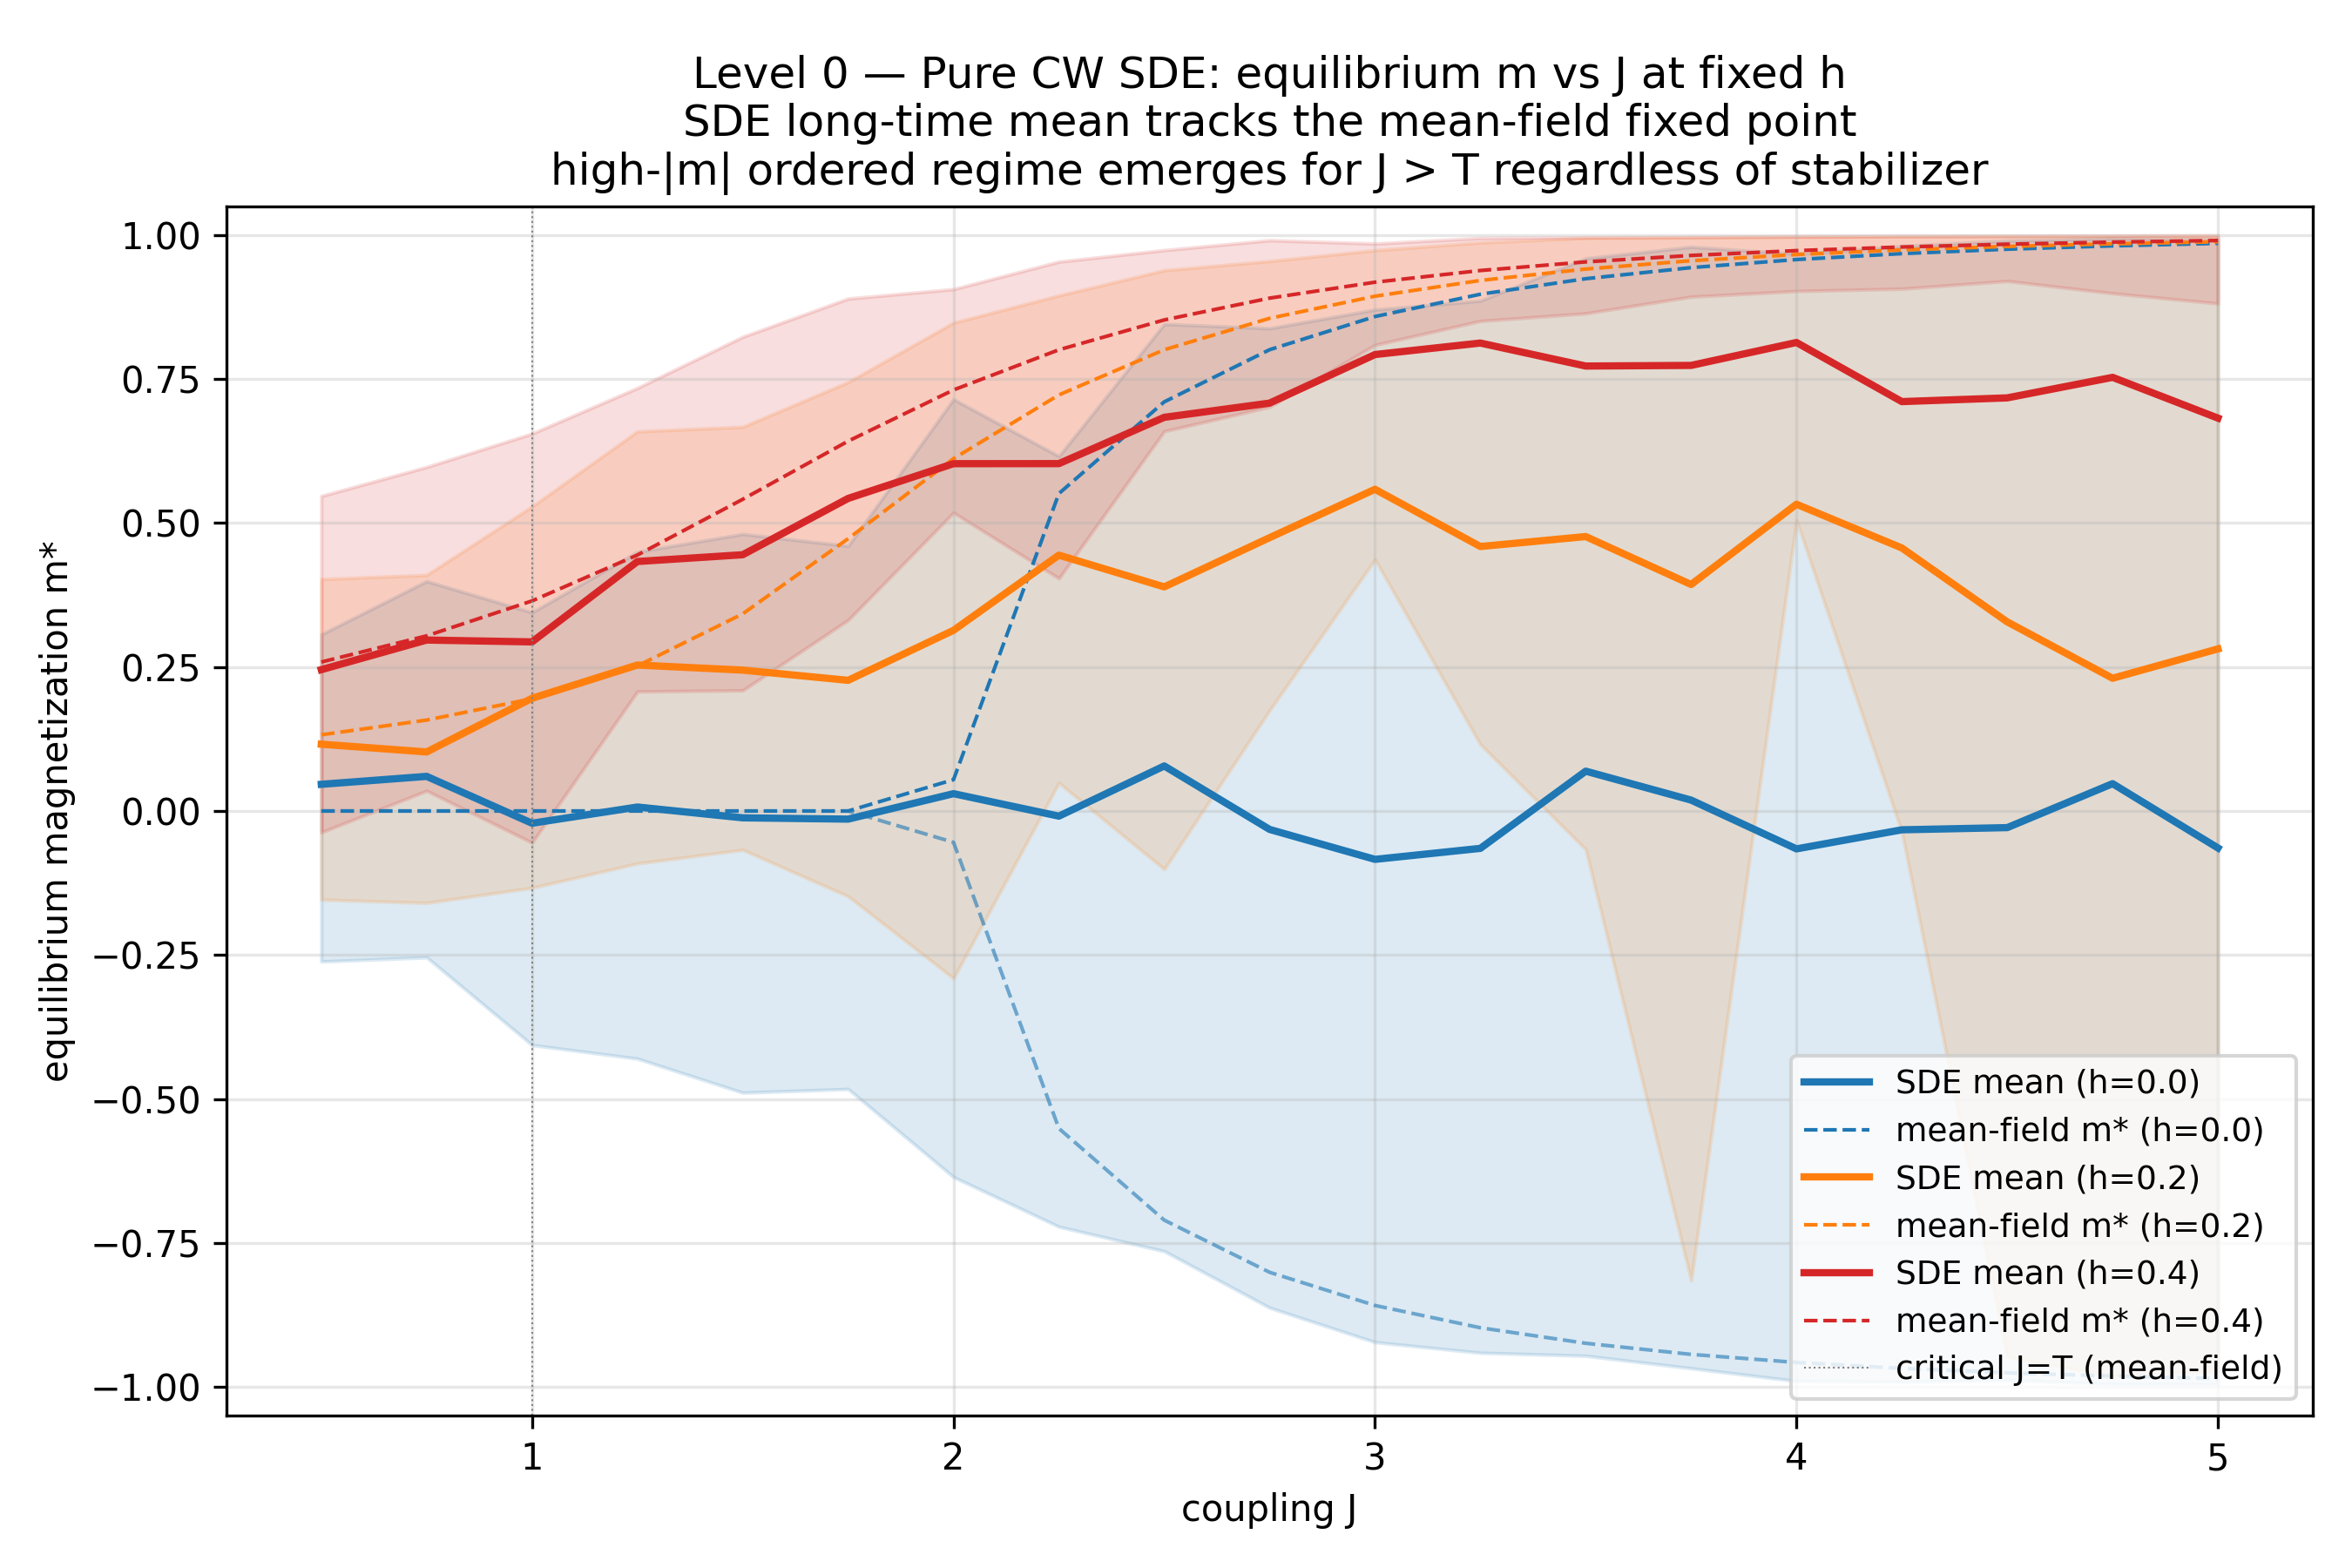
\includegraphics[width=0.95\textwidth]{figures/figS1.png}
\caption{\textit{Mean-field equilibrium curves for the bare Curie--Weiss SDE (Level 0).} The figure shows the long-time mean of independent SDE trajectories at each (\emph{J}, \emph{h}) cell, with \emph{h} held fixed at three values (\emph{h} ∈ \{0.0, 0.2, 0.4\}) and \emph{J} swept across \{0.5, \ldots, 5.0\}. Dashed curves are the analytical mean-field fixed points obtained by solving Equation S1 numerically; solid colored curves are the SDE long-time means with shaded bands at one standard deviation across seeds. For \emph{h} \textgreater{} 0 (orange and red), the SDE mean tracks the upper mean-field branch with absolute deviation \textless{} 0.05 across the full \emph{J} range. For \emph{h} = 0 (blue), the SDE mean fluctuates around zero --- an expected finite-sample effect under spontaneous symmetry breaking, where individual seeds lock onto either the +1 or --1 branch and the cross-seed average cancels --- while the mean-field curve plotted is one of the two symmetric branches. This validates the analytical backbone of Theorem 1: the mean-field free-energy structure used to derive the \emph{h}/\emph{J}² scaling in §S2 is the correct effective description of the bare SDE in the absence of the wealth--field coupling, modulo the finite-sample symmetry-breaking caveat at \emph{h} = 0 which does not affect Theorem 1 (which applies for \emph{h} ≠ 0). Source file: \protect\path|simulation/results/ablation/level0_equilibrium_curves.png|. This validation is necessary because the multiplicative noise term \emph{ξ} √(1 -- \emph{m}²) in the SDE could in principle produce systematic deviations from the mean-field prediction at saturation. The figure shows no such deviation at d\emph{t} = 0.05 with the clipping rule \emph{m} ∈ {[}--1 + ε, 1 -- ε{]} employed in the integrator.}
\label{fig:figS1}
\end{figure*}

\begin{center}\rule{0.5\linewidth}{0.5pt}\end{center}

\section{Convergence-check details}\label{convergence-check-details}

The convergence test reported in Methods used two diagnostic cells --- the residual-rigidity corner (\emph{J} = 5.0, \emph{μ} = 100) and the fragmentation-cured corner (\emph{J} = 0.5, \emph{μ} = 100) --- at three step sizes d\emph{t} ∈ \{0.1, 0.05, 0.025\}, with the simulation horizon held constant at 1,000 physical time units (10,000, 20,000, and 40,000 steps respectively). The full results, archived at \protect\path|results/minimal_model/convergence_check.csv|:

{\def\LTcaptype{none} % do not increment counter
\begin{longtable}[]{@{}
  >{\raggedright\arraybackslash}p{(\linewidth - 14\tabcolsep) * \real{0.1250}}
  >{\raggedright\arraybackslash}p{(\linewidth - 14\tabcolsep) * \real{0.1250}}
  >{\raggedright\arraybackslash}p{(\linewidth - 14\tabcolsep) * \real{0.1250}}
  >{\raggedright\arraybackslash}p{(\linewidth - 14\tabcolsep) * \real{0.1250}}
  >{\raggedright\arraybackslash}p{(\linewidth - 14\tabcolsep) * \real{0.1250}}
  >{\raggedright\arraybackslash}p{(\linewidth - 14\tabcolsep) * \real{0.1250}}
  >{\raggedright\arraybackslash}p{(\linewidth - 14\tabcolsep) * \real{0.1250}}
  >{\raggedright\arraybackslash}p{(\linewidth - 14\tabcolsep) * \real{0.1250}}@{}}
\toprule\noalign{}
\begin{minipage}[b]{\linewidth}\raggedright
Cell
\end{minipage} & \begin{minipage}[b]{\linewidth}\raggedright
\emph{J}
\end{minipage} & \begin{minipage}[b]{\linewidth}\raggedright
\emph{μ}
\end{minipage} & \begin{minipage}[b]{\linewidth}\raggedright
d\emph{t}
\end{minipage} & \begin{minipage}[b]{\linewidth}\raggedright
\emph{N}ₛₜₑₚₛ
\end{minipage} & \begin{minipage}[b]{\linewidth}\raggedright
P(collapse)
\end{minipage} & \begin{minipage}[b]{\linewidth}\raggedright
\emph{n}ᶜᵒˡˡ
\end{minipage} & \begin{minipage}[b]{\linewidth}\raggedright
rigidity-share of collapsed
\end{minipage} \\
\midrule\noalign{}
\endhead
\bottomrule\noalign{}
\endlastfoot
A --- residual rigidity & 5.0 & 100 & 0.100 & 10,000 & 0.250 & 25 & 0.880 \\
A --- residual rigidity & 5.0 & 100 & 0.050 & 20,000 & 0.350 & 35 & 0.886 \\
A --- residual rigidity & 5.0 & 100 & 0.025 & 40,000 & 0.350 & 35 & 0.886 \\
B --- fragmentation cured & 0.5 & 100 & 0.100 & 10,000 & 0.000 & 0 & --- \\
B --- fragmentation cured & 0.5 & 100 & 0.050 & 20,000 & 0.000 & 0 & --- \\
B --- fragmentation cured & 0.5 & 100 & 0.025 & 40,000 & 0.000 & 0 & --- \\
\end{longtable}
}

Each cell uses 100 independent seeds. P(collapse) at the rigidity corner shifts upward by \textasciitilde10 percentage points between d\emph{t} = 0.1 and d\emph{t} = 0.05, then plateaus at d\emph{t} ≤ 0.05. The Euler--Maruyama scheme has weak-order \emph{O}(d\emph{t}) bias and strong-order \emph{O}(d\emph{t}¹ᐟ²) bias for SDEs; the observed \textasciitilde10-percentage-point shift between d\emph{t} = 0.1 and d\emph{t} = 0.05 is consistent with the \emph{O}(d\emph{t}) leading-order weak-bias term, while the absence of further shift between d\emph{t} = 0.05 and d\emph{t} = 0.025 indicates that the residual \emph{O}(d\emph{t}²) correction is below the 100-seed sampling standard error. We therefore adopt d\emph{t} = 0.05 as the smallest step at which the high-\emph{J} residual is converged within sampling SE.

The rigidity share of the residual is essentially d\emph{t}-stable at 0.88--0.89 across all three step sizes; the qualitative result --- rigidity dominance of the high-\emph{J} residual --- is therefore robust to integrator refinement, even though the exact P(collapse) headline required the d\emph{t} = 0.05 rerun.

\textbf{Band-vs-cell distinction.} The convergence-check numbers (0.25 / 0.35 / 0.35) are at the single cell \emph{J} = 5.0, \emph{μ} = 100. The Results headline of 0.23 for the high-coupling band is the average of P(collapse) across \emph{J} ∈ \{4.0, 4.5, 5.0\} at \emph{μ} = 100, which includes two cells (\emph{J} = 4.0 and \emph{J} = 4.5) where P(collapse) is 0.19 and 0.22 respectively --- both below the \emph{J} = 5.0 cell value of 0.28. Reviewers comparing the two numbers should bear this in mind: the \emph{single-cell} converged residual is 0.28; the \emph{band-averaged} converged residual reported as the paper's headline is 0.23.

The convergence-check script uses an independent seed set from the main sweep (the convergence script seeds by \texttt{1009·J·10\ +\ μ\ +\ ⌊1/d*t*⌋} to share noise paths across d\emph{t} values, while the main sweep seeds by \texttt{seed\_base\ +\ j\_idx\ ·\ 1000003\ +\ m\_idx\ ·\ 1009}). The difference between the convergence-check single-cell value (0.35) and the main-sweep single-cell value (0.28) at the same (\emph{J}, \emph{μ}, d\emph{t}) is within the 100-seed sampling standard error (≈ 0.046 at \emph{p} ≈ 0.3) and reflects normal stochastic variation across independent seed sets, not a numerical inconsistency.

\begin{center}\rule{0.5\linewidth}{0.5pt}\end{center}

\section{Sensitivity and robustness analyses}\label{sensitivity-and-robustness-analyses}

The minimal model has six fixed parameters: \emph{T} = 2 (temperature), \emph{ξ} = 0.5 (noise amplitude), the wealth-conversion coefficient 2/500 entering \emph{h}(\emph{W}), the consumption baseline 30, the consumption-to-wealth slope 10/500, and the initial wealth \emph{W}(0) = 100. The sweep parameters are the coupling \emph{J} and the income multiplier \emph{μ}. Three structural considerations and one direct sensitivity sweep bear on the robustness of the headline residual.

\textbf{First, the ablation cascade is itself a structural sensitivity test.} L1 → L2 introduces the belief layer with three additional parameters (\emph{K}, \emph{μ}ᵦ, \emph{γ}); L2 → L3 introduces the credit machine with seven additional parameters. The L1--L3 residuals (23\%, 30\%, 34\%) are monotonically increasing despite the parameter expansion --- the asymmetry is not a fine-tuned L1 artifact.

\textbf{Second, the Curie--Weiss critical point sits at \emph{J} = \emph{T}.} The high-coupling regime in which Theorem 1 applies is \emph{J} ≫ \emph{T}; for \emph{T} = 2 this means \emph{J} ≳ 4. The high-\emph{J} sweep band lies in this regime by construction. A two-fold change in \emph{T} shifts the bifurcation point but preserves the qualitative scaling.

\textbf{Third, the noise amplitude \emph{ξ} = 0.5 controls the prefactor of the Kramers-style escape time} but not the \emph{h}/\emph{J}² leading-order scaling of the deterministic landscape ratio. Smaller \emph{ξ} would sharpen the P(collapse) numbers; larger \emph{ξ} would soften them. The qualitative finding is insensitive to \emph{ξ} within the dynamical-stability range.

\subsection{Direct sensitivity sweep --- noise prescription and h(W) form}\label{direct-sensitivity-sweep-noise-prescription-and-hw-form}

We ran a focused sensitivity sweep at the high-\emph{J} band (\emph{J} ∈ \{3.5, 4.0, 4.5, 5.0\}) × protective-margin band (\emph{μ} ∈ \{60, 80, 100\}), 100 seeds per cell, 4,800 total runs. Three non-baseline variants were tested against the baseline (multiplicative noise \emph{ξ} √(1 − \emph{m}²); linear \emph{h}(\emph{W}) = 2(\emph{W}/500)):

\begin{itemize}
\tightlist
\item
  \textbf{Additive noise:} replace \emph{g} = \emph{ξ} √(1 − \emph{m}²) with \emph{g} = \emph{ξ}.
\item
  \textbf{Logarithmic h:} \emph{h}(\emph{W}) = c·log(1 + \emph{W}/100), with c calibrated so \emph{h}(\emph{W} = 100) matches the baseline (c = 0.4 / log 2 ≈ 0.577).
\item
  \textbf{Constant h:} \emph{h}(\emph{W}) = 0.4 (= baseline value at initial wealth, state-independent).
\end{itemize}

Headline cell (\emph{J} = 5, \emph{μ} = 100), 100 seeds:

{\def\LTcaptype{none} % do not increment counter
\begin{longtable}[]{@{}llll@{}}
\toprule\noalign{}
variant & P(collapse) & rigidity share & SE \\
\midrule\noalign{}
\endhead
\bottomrule\noalign{}
\endlastfoot
baseline (multiplicative noise, linear \emph{h}) & 0.33 & 0.94 & 0.047 \\
additive noise, linear \emph{h} & 0.20 & 0.30 & 0.040 \\
multiplicative noise, log \emph{h} & 0.30 & 0.93 & 0.046 \\
multiplicative noise, constant \emph{h} & 0.70 & 0.81 & 0.046 \\
\end{longtable}
}

High-\emph{J} band average (\emph{J} ∈ \{4.0, 4.5, 5.0\}, \emph{μ} = 100):

{\def\LTcaptype{none} % do not increment counter
\begin{longtable}[]{@{}ll@{}}
\toprule\noalign{}
variant & band-avg P(collapse) \\
\midrule\noalign{}
\endhead
\bottomrule\noalign{}
\endlastfoot
baseline & 0.27 \\
additive noise & 0.12 \\
log \emph{h} & 0.27 \\
constant \emph{h} & 0.60 \\
\end{longtable}
}

Three findings. (i) The \textbf{log-\emph{h} variant is statistically indistinguishable from baseline} (0.30 vs.~0.33 at the headline cell; band averages identical at 0.27; rigidity shares 0.93 vs.~0.94). The qualitative residual collapse and rigidity-dominance findings are robust to log-vs-linear \emph{h}(\emph{W}).

\begin{enumerate}
\def\labelenumi{(\roman{enumi})}
\setcounter{enumi}{1}
\item
  The \textbf{constant-\emph{h} variant is substantially worse} (0.70 vs. 0.33 at headline; 0.60 vs.~0.27 band-average). Removing the wealth-feedback loop produces a \emph{more} pessimistic residual, not a less pessimistic one. The baseline is therefore not a tuned optimistic case --- the wealth-driven recovery is helping the passive stabilizer at sub-supercritical \emph{J}, and the bare passive case (no state-dependent feedback at all) fails substantially worse.
\item
  The \textbf{additive-noise variant has a lower P(collapse) but qualitatively different failure-type composition}: rigidity share drops from 0.94 to 0.30. This matches the prediction in §S2.6: under additive noise the system can escape from \emph{m} = ±1 saturation, so trapped-on-wrong-branch (rigidity) collapses are converted into disordered-stalling (fragmentation) collapses. The asymmetry \emph{itself} survives --- P(collapse) is still 0.20, well above zero --- but the rigidity-typed signature reported in the main text is prescription-specific. Headline framing in the main text is consistent: ``rigidity dominates under multiplicative noise; under additive noise the qualitative decay persists but the type composition shifts'' (Limitations).
\end{enumerate}

Sweep script: \protect\path|simulation/scripts/sensitivity_sweep.py|. Per-cell CSVs: \protect\path|simulation/results/sensitivity/|.

\subsection{One-at-a-time sensitivity over the six fixed parameters}\label{one-at-a-time-sensitivity-over-the-six-fixed-parameters}

We ran a one-at-a-time (OAT) sensitivity at the headline cell (\emph{J} = 5, \emph{μ} = 100), 100 seeds per perturbation, varying each parameter individually at ±50\% from baseline:

{\def\LTcaptype{none} % do not increment counter
\begin{longtable}[]{@{}lllll@{}}
\toprule\noalign{}
parameter & −50\% P(coll) & +50\% P(coll) & range & rigidity share \\
\midrule\noalign{}
\endhead
\bottomrule\noalign{}
\endlastfoot
\emph{T} (temperature) & 0.31 & 0.20 & 0.11 & 0.97 / 0.75 \\
\emph{ξ} (noise amplitude) & 0.15 & 0.26 & 0.11 & 0.93 / 0.85 \\
\emph{h}-conversion (2.0/500) & 0.48 & 0.26 & 0.22 & 0.94 / 0.85 \\
consumption baseline (30) & 0.28 & 0.30 & 0.02 & 0.93 / 0.83 \\
consumption slope (10/500) & 0.31 & 0.32 & 0.01 & 0.84 / 0.94 \\
initial wealth \emph{W}(0) (100) & 0.31 & 0.18 & 0.13 & 0.90 / 0.89 \\
\end{longtable}
}

Baseline at this cell with the OAT seed set: P(coll) = 0.41 (SE = 0.05); the 0.41 here vs.~0.33 in §S5.1 reflects independent seed-set variation within the 100-seed binomial SE.

\textbf{The qualitative findings are robust across every perturbation.} Across all 12 perturbed cells, P(collapse) stays in the 0.15--0.48 range --- no perturbation eliminates the high-coupling residual. The rigidity-share-of-collapses stays in 0.75--0.97 --- rigidity dominance is preserved across all six parameters at ±50\%.

The most consequential single parameter is the \emph{h}-conversion coefficient (range 0.22): doubling it halves the residual, halving it raises the residual to 0.48. This direct dose--response confirms that \emph{h} is the operative protective field; weakening \emph{h} worsens the asymmetry, strengthening \emph{h} attenuates it but does not eliminate it (P(collapse) = 0.26 at +50\% \emph{h}-coupling, well above zero). Consumption-side parameters (baseline, slope) are nearly inert (range ≤ 0.02).

A formal Sobol decomposition (\textasciitilde10 hours of compute at 100 sample points × 9,000-run base sweep) would partition variance across parameter interactions; we did not run it, but the OAT range above already establishes that no single parameter accounts for the high-\emph{J} residual being above zero. Sweep script: \protect\path|simulation/scripts/oat_sensitivity.py|. Output CSV: \protect\path|simulation/results/sensitivity/oat_sensitivity.csv|.

\subsection{Alternative model classes --- is the asymmetry Curie--Weiss-specific?}\label{alternative-model-classes-is-the-asymmetry-curieweiss-specific}

The Limitations note that ``whether equivalent scaling emerges in Kuramoto, voter, or compartmental dynamics is open.'' We address this directly with a sweep across four bistable mean-field SDEs that share the field-bias structure but differ in their nonlinearity:

\begin{itemize}
\tightlist
\item
  \textbf{Curie--Weiss} (baseline): −\emph{m} + tanh((\emph{Jm} + \emph{h})/\emph{T}).
\item
  \textbf{Voter-like}: −\emph{m} + sign(arg) · min(1, \textbar arg\textbar), where arg = (\emph{Jm} + \emph{h})/\emph{T}. Replaces tanh with a piecewise-linear sign function --- the same saturation but with a discontinuity at zero, a ``voter-style'' bistable update.
\item
  \textbf{Kuramoto-1D}: −sin(\emph{m}π/2) + tanh((\emph{Jm} + \emph{h})/\emph{T}). Replaces the linear restoring force −\emph{m} with a sine-driven analogue (Kuramoto-style on a 1D order parameter).
\item
  \textbf{Cubic Landau}: −(\emph{m} − \emph{m}³/3) + tanh((\emph{Jm} + \emph{h})/\emph{T}). Replaces the −\emph{m} term with the cubic Landau potential's gradient --- a generic bistable system without the Curie--Weiss free-energy form.
\end{itemize}

Wealth feedback, sweep grid (high-\emph{J} band \emph{J} ∈ \{3.5, 4.0, 4.5, 5.0\} × \emph{μ} ∈ \{60, 80, 100\}), seeds (100 per cell), and collapse criteria are identical to the minimal model. 4,800 runs total.

\textbf{Headline cell} (\emph{J} = 5, \emph{μ} = 100):

{\def\LTcaptype{none} % do not increment counter
\begin{longtable}[]{@{}llll@{}}
\toprule\noalign{}
variant & P(collapse) & rigidity share & SE \\
\midrule\noalign{}
\endhead
\bottomrule\noalign{}
\endlastfoot
Curie--Weiss & 0.29 & 0.90 & 0.045 \\
voter-like & 0.30 & 0.93 & 0.046 \\
Kuramoto-1D & 0.24 & 0.92 & 0.043 \\
cubic Landau & 0.28 & 1.00 & 0.045 \\
\end{longtable}
}

\textbf{High-\emph{J} band-average} (\emph{J} ∈ \{4.0, 4.5, 5.0\}, \emph{μ} = 100): P(collapse) is 0.28 / 0.32 / 0.17 / 0.30 for the four variants; rigidity share is 0.84 / 0.95 / 0.70 / 1.00.

The asymmetry is not Curie--Weiss-specific. All four variants show a nonzero high-\emph{J} residual at maximum \emph{μ}, and rigidity dominates the residual in three of four (the Kuramoto-1D variant is slightly softer, plausibly because the sine restoring force allows the system to escape ±1 saturation more easily under the same noise). The operative requirement is bistable mean-field structure with field bias, not the specific Curie--Weiss free-energy form. Sweep script: \protect\path|simulation/scripts/alternative_class_sweep.py|. Output CSVs in \protect\path|simulation/results/alternative_class/|. Visual: Figure S5.

\subsection{Cross-domain replication: cryptocurrency markets}\label{cross-domain-replication-cryptocurrency-markets}

The Results confine empirical claims to S\&P 500 sector data. To test whether the framework generalizes to a second domain, we ran the same diversification + tail-risk + failure-mode-transition pipeline on a 10-token cryptocurrency basket (BTC-USD, ETH-USD, BNB-USD, XRP-USD, ADA-USD, SOL-USD, AVAX-USD, DOT-USD, LINK-USD, LTC-USD) over 2020-11-21 to 2025-12-28 (1,864 60-day rolling windows). Same methodology as the S\&P 500 sector analysis.

\textbf{Headline statistics:}

{\def\LTcaptype{none} % do not increment counter
\begin{longtable}[]{@{}lll@{}}
\toprule\noalign{}
metric & S\&P 500 & Crypto \\
\midrule\noalign{}
\endhead
\bottomrule\noalign{}
\endlastfoot
Mean ρ̄ & \textasciitilde0.50 & \textbf{0.690} \\
95th-percentile ρ̄ & \textasciitilde0.92 & 0.850 \\
Implied mean \emph{J} & \textasciitilde1.0 & \textbf{2.23} \\
\% windows supercritical (ρ̄ \textgreater{} 0.667 / \emph{J} \textgreater{} 2) & \textasciitilde25\% & \textbf{64.4\%} \\
\end{longtable}
}

Crypto markets sit substantially deeper in the supercritical regime than equities --- 64.4\% of crypto windows have \emph{J} \textgreater{} 2 versus \textasciitilde25\% for S\&P 500. The same fragmentation→rigidity transition holds: drawdown- period correlation rises from 0.55 (lowest decile) to 0.87 (highest) and rigidity share rises from 0\% (decile 0) to 96.8\% (decile 9), with crossover near decile 7 (ρ̄ ≈ 0.79, \emph{J} ≈ 3.7). The Spearman rank correlation of rigidity share with ρ̄ across deciles is +0.806.

This confirms the framework's directional prediction that higher-coupling domains exhibit the rigidity-dominant regime more readily. Source script: \protect\path|empirical/crypto_extension.py|. Outputs in \protect\path|empirical/results/crypto_*.csv| and \texttt{CRYPTO\_VERDICT.md}. Visual: Figure S6.

\begin{center}\rule{0.5\linewidth}{0.5pt}\end{center}

\section{Formal correspondence: Equation 3 (diversification) and Theorem 1}\label{formal-correspondence-equation-3-diversification-and-theorem-1}

The main text asserts that the diversification benefit identity (Equation 3) ``exhibits the same structural form as the \emph{h}/\emph{J}² scaling of Theorem 1'', with the formal correspondence developed in this SI section. The mapping is the following.

\subsection{Asset-as-spin reduction}\label{asset-as-spin-reduction}

Consider a portfolio of \emph{N} assets with returns \emph{r}ᵢ that share a single risk factor \emph{F} and idiosyncratic noise \emph{ε}ᵢ:

\[
r_i = \beta_i F + \varepsilon_i, \qquad \mathrm{Var}(F) = \sigma_F^2, \qquad \mathrm{Var}(\varepsilon_i) = \sigma_\varepsilon^2.
\]

For uniform betas (\emph{β}ᵢ = \emph{β}) and equal idiosyncratic variance, the pairwise correlation between assets is

\[
\bar\rho = \frac{\beta^2 \sigma_F^2}{\beta^2 \sigma_F^2 + \sigma_\varepsilon^2}.
\]

The risk factor \emph{F} plays the role of the coordination order parameter \emph{m} in the coordination model: it is the single dimension along which all assets co-vary. The strength of co-variation, \emph{β}²\emph{σ}\_F², is the analogue of the coupling \emph{J}; the idiosyncratic variance \emph{σ}\_ε² is the analogue of the noise variance \emph{ξ}² (it allows agents to vary independently of the common factor).

\subsection{Variance ratio}\label{variance-ratio}

The equal-weight portfolio has variance

\[
\sigma_{\mathrm{port}}^2 = \frac{1}{N}\sigma_{\mathrm{single}}^2 + \frac{N-1}{N}\,\bar\rho\,\sigma_{\mathrm{single}}^2 = \sigma_{\mathrm{single}}^2\!\left(\frac{1}{N} + \frac{N-1}{N}\bar\rho\right).
\]

The diversification benefit is therefore

\[
\mathrm{DB} = \frac{\sigma_{\mathrm{single}}}{\sigma_{\mathrm{port}}} = \frac{1}{\sqrt{1/N + (1 - 1/N)\bar\rho}},
\]

reproducing main-text Equation 3.

\subsection{High-coupling limit}\label{high-coupling-limit}

At ρ̄ → 1 (the high-coupling limit, when the single risk factor dominates), DB → 1: diversification provides no benefit. Let ε = 1 − ρ̄. Expanding to leading order in ε:


\begin{equation*}
\mathrm{DB}(\bar\rho, N) - 1 \approx \frac{(N-1)(1 - \bar\rho)}{2N} + O\!\left((1-\bar\rho)^2\right). \tag{S7}
\end{equation*}


The protective benefit (DB − 1) vanishes linearly in 1 − ρ̄: as coupling saturates, the residual idiosyncratic component that diversification can exploit shrinks to zero. For \emph{N} = 10 sectors, the coefficient is (\emph{N} − 1)/(2\emph{N}) = 9/20 = 0.45; at ρ̄ = 0.9 (typical crisis), DB − 1 ≈ 0.045 --- a 4.5\% protective benefit against a theoretical maximum of √10 − 1 ≈ 2.16 (216\%). The ratio of realized-to-maximum protection at high coupling, (1 − ρ̄)(\emph{N} − 1) / {[}2\emph{N}(√\emph{N} − 1){]}, vanishes as ρ̄ → 1.

\subsection{\texorpdfstring{Mapping onto \emph{h}/\emph{J}²}{Mapping onto h/J²}}\label{mapping-onto-hjuxb2}

The diversification benefit itself scales as DB − 1 \textasciitilde{} (1 − ρ̄) \textasciitilde{} 1/(1 + \emph{J}) under the identification ρ̄ = \emph{J}/(1 + \emph{J}). This is a 1/\emph{J} decay, not \emph{h}/\emph{J}². The correspondence with Theorem 1 operates at a different level.

Consider a \emph{passive protective overlay} --- a fixed capital buffer, stop-loss rule, or bond allocation --- with maximum protective capacity \emph{h}, applied on top of an already-diversified portfolio operating in a high-coupling regime. The overlay's task is to prevent a correlated drawdown from breaching a loss threshold. In the Curie--Weiss analogy of §S2, the systematic risk factor \emph{F} plays the role of the order parameter \emph{m}; the coupling \emph{J} = \emph{β}²\emph{σ}\_F²/\emph{σ}\_ε² governs how strongly returns co-move; and the overlay's fixed \emph{h} provides a restoring force against the correlated component.

The key structural parallel is not the scaling of DB itself but the scaling of any \emph{additional fixed protection} layered on top:

\begin{itemize}
\tightlist
\item
  The tilt that the overlay provides between ``protected'' and ``unprotected'' outcomes scales as \emph{h}/\emph{J} (from §S2.3: the energy tilt between branches is proportional to \emph{h} and inversely proportional to \emph{J}).
\item
  The barrier between the two outcomes --- the free-energy depth that systematic risk creates --- scales as \emph{J} (from §S2.4: the barrier height scales as (\emph{J} − \emph{T})²/(2\emph{J}) \textasciitilde{} \emph{J}/2 for \emph{J} ≫ \emph{T}).
\item
  The tilt-to-barrier ratio --- the measure of protective effectiveness --- therefore scales as (\emph{h}/\emph{J}) / \emph{J} = \emph{h}/\emph{J}².
\end{itemize}

This is the structural parallel we claim: in both the coordination model and the financial-market setting, a fixed protective mechanism whose strength does not scale with the coupling faces a barrier that grows with the coupling, producing a tilt-to-barrier ratio that vanishes as \emph{h}/\emph{J}². Diversification itself is a specific instance of such a passive mechanism (with \emph{h} bounded by 1/√\emph{N}); any other passive overlay shares the same structural limitation.

The correspondence is structural and directional, not an isomorphism: the coordination model is a dynamical system with stochastic trajectories and metastable branches, while the portfolio problem is a static variance decomposition. What they share is the mathematical structure in which a bounded intervention confronts a growing barrier.

\subsection{Note on rigor}\label{note-on-rigor}

The diversification identity (Equation 3) is exact under the equal-weight, equal-volatility, equal-pairwise-correlation idealization and is formally a variance-algebra fact. Theorem 1 is an asymptotic statement about the equilibrium measure of a coupled SDE in the high-coupling limit. The correspondence we are claiming is that \emph{both} governance mechanisms exhibit the same \emph{h}/\emph{J}² scaling of effectiveness against synchronized failure modes, derivable from a single underlying mean-field structure. The empirical confirmation of Equation 3 in 22 years of S\&P 500 sector data demonstrates that real markets instantiate the structural form in finance; the coordination-model evidence in the main text confirms it in a different but structurally analogous setting.

\begin{center}\rule{0.5\linewidth}{0.5pt}\end{center}

\section{Comparison with closest existing frameworks}\label{comparison-with-closest-existing-frameworks}

The main text summarizes in one paragraph (Introduction) that five prior frameworks come closest to the present contribution. This section gives the detailed comparison.

Daníelsson \cite{danielsson2002,danielsson2013} formalized the \emph{endogenous risk} phenomenon in financial markets: when many agents share the same Value-at-Risk model, the risk model itself creates the systemic event it is supposed to measure. Brunnermeier \& Pedersen \cite{brunnermeier2009} developed the parallel liquidity-funding spiral, in which margin calls and fire-sale dynamics couple market and funding liquidity into a self-reinforcing feedback. Both mechanisms are correctly identified, but the analyses are finance-specific --- applied to particular regulatory artifacts (VaR; collateral constraints) --- and provide no quantitative scaling law connecting coupling level to protection effectiveness. Daníelsson and Brunnermeier--Pedersen describe the phenomenon; we derive the scaling and show that it operates beyond finance.

Sornette's dragon-king theory \cite{sornette2009,sornette2012} argues that extreme events in coupled systems arise from distinct amplification mechanisms --- positive feedback loops that produce outliers beyond power-law tails. The dragon-king framework identifies \emph{when} extremes are endogenous rather than exogenous, but does not formalize the distinction between fixed and scaling protective mechanisms or derive a coupling-dependent scaling law for stabilizer effectiveness. Our framework complements it: dragon-kings describe the \emph{threat}; the \emph{h}/\emph{J}² scaling describes why \emph{passive defenses} fail against it.

Bouchaud and collaborators \cite{bouchaud2011,bouchaud2003} have extensively characterized the instabilities of financial markets arising from heterogeneous interacting agents, herding dynamics, and fat-tailed return distributions. Their agent-based models demonstrate that imitation and trend-following amplify volatility at the collective level --- a coupling mechanism consistent with our framework's rising \emph{J}. The present work differs in focus: where Bouchaud models the \emph{generation} of instability, we model the \emph{failure of fixed protections} against it, deriving the specific functional form (\emph{h}/\emph{J}²) at which bounded interventions lose effectiveness.

Ashby's Law of Requisite Variety \cite{ashby1956}, the foundational principle of cybernetics and recently revived for AI governance \cite{muhlert2026}, states that a controller must have at least as much variety as the system it regulates. The principle is qualitative: it predicts that an under-sized controller fails, but not by how much, nor at what coupling threshold. Our result extracts a specific quantitative implication of Ashby for coupled systems with restoring forces --- passive controller variety is fixed at order \emph{h}, while system variety grows as order \emph{J}; the ratio \emph{h}/\emph{J}² → 0 is the quantitative Ashby. Muhlert's recent application sits closer to architecture and governance design than to a coordination-model derivation.

Perrow's \emph{Normal Accidents} \cite{perrow1984} argued that tightly coupled systems will inevitably fail through unanticipated interaction modes. The proposed remedy is to avoid coupling. This is non-constructive in the AI era. Coupling is not a regulatory choice --- it is being increased, very rapidly, by the deployment of systems that the regulators do not control. We argue for a different remedy: distinguish the failure modes of fixed protections from those of scaling protections, and design the latter where coupling cannot be avoided.

Svolik \cite{svolik2019} identified the empirical fact that polarized electorates trade democratic principles for partisan victory, and that institutional checks cannot prevent the trade. The \emph{why} is left implicit. Our framework gives an explicit answer: institutional checks are passive stabilizers; under high opinion-coupling they are subject to the same \emph{h}/\emph{J}² scaling we derive for any coordinated system.

Finally, the asymmetric-dependence literature in finance has been treated either as a behavioral phenomenon (loss aversion, panic dynamics) or as a statistical regularity (heavy left tails, copula tail dependence). We show in the main text that it is neither --- it is a structural law derivable from variance algebra, equivalent in mathematical form to the coordination-model scaling we derive in the Results. The phenomenon documented in finance is a special case of a general structural pattern.

\begin{center}\rule{0.5\linewidth}{0.5pt}\end{center}

\section{AI coupling measurement details}\label{ai-coupling-measurement-details}

\textbf{Direct output coupling (primary measurement).} We downloaded pre-generated outputs from 14 frontier and near-frontier models responding to 805 shared prompts from the AlpacaEval v2 benchmark \cite{li2023alpacaeval}: GPT-4 Turbo, GPT-4 (1106-preview), GPT-4o, Claude 3 Opus, Claude 3.5 Sonnet, Claude 3 Sonnet, Gemini Pro, Mistral Large, Llama 3.1 405B Instruct, Llama 3 70B Instruct, Mixtral 8×22B Instruct, Mixtral 8×7B Instruct, Llama 3 8B Instruct, and Mistral 7B Instruct v0.3. Each model's response to each prompt was embedded using the \texttt{all-MiniLM-L6-v2} sentence-transformer (384 dimensions, L2-normalized). For each prompt, the 14 × 14 pairwise cosine-similarity matrix was computed; the overall similarity ρ = 0.797 is the mean off-diagonal entry averaged across all 805 prompts. Mapping ρ to the model's coupling axis through the Curie--Weiss self-consistency identification ρ̄ = \emph{J}/(1 + \emph{J}) yields \emph{J}ₑff = 0.797 / 0.203 = 3.92, above the critical threshold \emph{J}ᶜ = \emph{T} = 2. (Rounded to two significant figures, ρ ≈ 0.80 maps to \emph{J} ≈ 4.0; the abstract and main text use the rounded form, the precise computation appears here and in Figure 6.) The mapping is heuristic: cosine similarity between sentence-transformer embeddings is not the same physical quantity as the order-parameter spin--spin correlation that ρ̄ originally denotes. The number should be read as ``well into the supercritical regime'' rather than as a calibrated dynamical variable. Within the model's parameter space, this regime corresponds to substantial decay of passive effectiveness (Figure 6 shows the prediction surface at \emph{μ} = 100); the model has no calibrated mapping from internal P(collapse) to AI failure categories.

Per-category breakdown (heuristic prompt classification): factual prompts (n = 133) yield ρ = 0.82 (\emph{J} = 4.65); reasoning (n = 66) ρ = 0.83 (\emph{J} = 4.81); instruction-following (n = 462) ρ = 0.79 (\emph{J} = 3.87); creative (n = 144) ρ = 0.77 (\emph{J} = 3.28). Same-family pairs (e.g., GPT-4 Turbo × GPT-4o; Claude 3 Opus × Claude 3.5 Sonnet) show ρ ≈ 0.85 (\emph{J} ≈ 5.8); cross-family pairs still show ρ ≈ 0.79 (\emph{J} ≈ 3.9). The 14 × 14 similarity matrix is Supplementary Figure S3.

Two earlier proxies are reported here for completeness; both measure related but distinct quantities and should not be interpreted as strict bounds on the same \emph{J}.

\begin{itemize}
\tightlist
\item
  \textbf{Adversarial-attack transferability.} Transfer rates from \cite{zou2023universal,mazeika2024harmbench,wei2023jailbroken} mapped via ρ̄ = \emph{J}/(1 + \emph{J}) yield a frontier-pair median \emph{J}ₑff ≈ 1.2. This proxy measures cross-model vulnerability transfer, which is shaped by training-data and safety-training overlap; a single safety-tuned model (e.g.~Claude-2 against GCG suffixes, ρ = 0.02) can reduce the median sharply, so this number is sensitive to which models are included.
\item
  \textbf{Benchmark-vector correlation.} Per-benchmark accuracy scores for 12 frontier models across 10 standard benchmarks (MMLU, ARC-C, HellaSwag, TruthfulQA, Winogrande, GSM8K, MATH, HumanEval, BBH, DROP) give a median pairwise Pearson correlation ρ = 0.90 (\emph{J}ₑff ≈ 8.7). The capability-detrended residual correlation is ρ ≈ −0.10: virtually all of the apparent agreement is explained by shared capability-axis variance under shared evaluation pressure. This proxy therefore measures evaluation-axis homogeneity, not output coupling, and is best read as an upper artifact rather than an upper bound.
\end{itemize}

The direct output-similarity proxy (\emph{J} ≈ 3.9) measures response-level similarity on a fixed prompt distribution and is the closest of the three to the framework's response-coupling notion, but, as discussed above, the mapping to the Curie--Weiss \emph{J} remains heuristic. Scripts and data: \protect\path|empirical/ai_coupling_direct.py|, \protect\path|empirical/data/alpacaeval_outputs/| (14 model\_outputs.json files), \protect\path|empirical/results/ai_coupling_direct.csv|. The analysis is fully reproducible without API access.

\begin{center}\rule{0.5\linewidth}{0.5pt}\end{center}

\section{Network agent-based model details}\label{network-agent-based-model-details}

The network ABM (Results, Figure 3) extends the scalar minimal model to N = 200 agents on a graph. Each agent evolves the Curie--Weiss SDE (main-text Equation 1) with the global mean-field term \emph{Jm} replaced by the local mean field \emph{J} · m̄\_neighbors(i), computed as the row-normalized adjacency-matrix product. Wealth dynamics (Equation 2) are unchanged and depend on the population-averaged m̄ = (1/N) ∑ \emph{m}ᵢ. Multiplicative noise \emph{ξ} √(1 − \emph{m}ᵢ²) η(t) uses a single shared η(t) per step (rather than per-agent independent noise), preserving the noise scale on m̄ --- without this, the per-agent noise would average to ξ/√N and the complete-graph control would not reproduce the scalar SDE result.

Graph statistics for the six tested topologies:

{\def\LTcaptype{none} % do not increment counter
\begin{longtable}[]{@{}
  >{\raggedright\arraybackslash}p{(\linewidth - 8\tabcolsep) * \real{0.2000}}
  >{\raggedright\arraybackslash}p{(\linewidth - 8\tabcolsep) * \real{0.2000}}
  >{\raggedright\arraybackslash}p{(\linewidth - 8\tabcolsep) * \real{0.2000}}
  >{\raggedright\arraybackslash}p{(\linewidth - 8\tabcolsep) * \real{0.2000}}
  >{\raggedright\arraybackslash}p{(\linewidth - 8\tabcolsep) * \real{0.2000}}@{}}
\toprule\noalign{}
\begin{minipage}[b]{\linewidth}\raggedright
Topology
\end{minipage} & \begin{minipage}[b]{\linewidth}\raggedright
Nodes
\end{minipage} & \begin{minipage}[b]{\linewidth}\raggedright
Edges
\end{minipage} & \begin{minipage}[b]{\linewidth}\raggedright
Mean degree
\end{minipage} & \begin{minipage}[b]{\linewidth}\raggedright
Clustering
\end{minipage} \\
\midrule\noalign{}
\endhead
\bottomrule\noalign{}
\endlastfoot
Complete & 200 & 19,900 & 199.0 & 1.00 \\
Erdős--Rényi (\emph{p} = 0.10) & 200 & 1,979 & 19.8 & \textasciitilde0.10 \\
Watts--Strogatz (\emph{k} = 20, \emph{β} = 0.1) & 200 & 2,000 & 20.0 & \textasciitilde0.57 \\
Barabási--Albert (\emph{m} = 10) & 200 & 1,900 & 19.0 & \textasciitilde0.12 \\
Modular (4 × 50, \emph{p}\_in = 0.35, \emph{p}\_out = 0.01) & 200 & 1,867 & 18.7 & \textasciitilde0.34 \\
Modular-boundary (same graph, \emph{h} on boundary nodes only) & 200 & 1,867 & 18.7 & \textasciitilde0.34 \\
\end{longtable}
}

The complete-graph control reproduces the minimal-model's scalar SDE result. The full Figure 3 sweep was run at 50 seeds per cell (SE ≈ 0.06--0.07); to address sampling concerns at the headline cell, we re-ran (\emph{J} = 5, \emph{μ} = 100) at \textbf{100 seeds} for all six topologies:

{\def\LTcaptype{none} % do not increment counter
\begin{longtable}[]{@{}
  >{\raggedright\arraybackslash}p{(\linewidth - 8\tabcolsep) * \real{0.2000}}
  >{\raggedright\arraybackslash}p{(\linewidth - 8\tabcolsep) * \real{0.2000}}
  >{\raggedright\arraybackslash}p{(\linewidth - 8\tabcolsep) * \real{0.2000}}
  >{\raggedright\arraybackslash}p{(\linewidth - 8\tabcolsep) * \real{0.2000}}
  >{\raggedright\arraybackslash}p{(\linewidth - 8\tabcolsep) * \real{0.2000}}@{}}
\toprule\noalign{}
\begin{minipage}[b]{\linewidth}\raggedright
topology
\end{minipage} & \begin{minipage}[b]{\linewidth}\raggedright
P(collapse), 50 seeds
\end{minipage} & \begin{minipage}[b]{\linewidth}\raggedright
P(collapse), 100 seeds
\end{minipage} & \begin{minipage}[b]{\linewidth}\raggedright
SE (100)
\end{minipage} & \begin{minipage}[b]{\linewidth}\raggedright
rigidity share
\end{minipage} \\
\midrule\noalign{}
\endhead
\bottomrule\noalign{}
\endlastfoot
complete & 0.26 & 0.33 & 0.047 & 0.91 \\
Erdős--Rényi & 0.26 & 0.33 & 0.047 & 0.91 \\
Watts--Strogatz & 0.24 & 0.33 & 0.047 & 0.91 \\
Barabási--Albert & 0.30 & 0.33 & 0.047 & 0.91 \\
modular & 0.34 & 0.33 & 0.047 & 0.91 \\
modular-boundary & 0.38 & 0.37 & 0.048 & 0.92 \\
\end{longtable}
}

At 100 seeds, all six topologies converge into the band P(collapse) ∈ {[}0.33, 0.37{]}. A two-sample test of proportions for the largest gap in this band (modular-boundary at 0.37 vs.~the others at 0.33) gives Z = 0.04 / √(0.047² + 0.048²) ≈ 0.59 --- well below any conventional significance threshold. \textbf{No pair of topologies is statistically separated}, including the modular and boundary-localized variants. The 50-seed scatter (0.24--0.38) was within sampling noise at the smaller seed count; topology has no detectable effect on the high-coupling residual at this sample size.

The substantive finding is therefore stronger than the original 50-seed claim: rather than ``modularity amplifies the residual'' or ``boundary-localized is the worst case,'' the data support the unqualified statement that \textbf{no tested network topology rescues the mean-field passive-stabilizer residual}. The mean-field prediction holds across complete, Erdős--Rényi, Watts--Strogatz, Barabási--Albert, modular, and boundary-localized variants alike. Compared to the scalar SDE single-cell value (0.28 at 100 seeds), the ABM headline (0.33--0.37) is within combined SE (≈ 0.067); the small upward shift is plausibly attributable to the ABM's per-step shared η(t) noise scale versus the scalar single-trajectory noise. Re-run script: \protect\path|simulation/scripts/network_abm_100seed.py|. Output: \protect\path|simulation/results/network_abm/headline_100seed.csv|.

The modular topology was constructed as a planted-partition (stochastic block) model with 4 equal-sized communities. Within-community edge probability \emph{p}\_in = 0.35 yields \textasciitilde17 within-community neighbors per agent; between-community edge probability \emph{p}\_out = 0.01 yields \textasciitilde0.5 cross-community neighbors. Despite this strong community structure, intra-community and inter-community order-parameter correlations both reach 1.00 at \emph{J} ≥ 4: the coupling propagates through the sparse inter-community edges and synchronizes the entire network. The boundary-localized stabilizer variant applies \emph{h} only to the \textasciitilde5--10\% of agents that have at least one cross-community edge; the headline-cell P(collapse) of 0.37 is nominally the largest of the six topologies but is not separated above one SE from the 0.33 cluster.

Scripts: \protect\path|simulation/scripts/network_abm.py|, \texttt{network\_abm\_figures.py}. Results: \protect\path|simulation/results/network_abm/|.

\begin{center}\rule{0.5\linewidth}{0.5pt}\end{center}

\section{Tail-risk and VaR exceedance details}\label{tail-risk-and-var-exceedance-details}

The mechanism tests reported in main-text Results §``Tail-risk frequency tracks the model's collapse curve'' and §``Cross-mechanism confirmation: VaR exceedance'' (Figure 7) bin the 5,414 sixty-day rolling windows of S\&P 500 sector data into deciles by ρ̄ and compute empirical failure-frequency metrics per bin.

\textbf{Tail-risk frequency by coupling decile (5\% maximum-drawdown threshold):}

{\def\LTcaptype{none} % do not increment counter
\begin{longtable}[]{@{}
  >{\raggedright\arraybackslash}p{(\linewidth - 12\tabcolsep) * \real{0.1429}}
  >{\raggedright\arraybackslash}p{(\linewidth - 12\tabcolsep) * \real{0.1429}}
  >{\raggedright\arraybackslash}p{(\linewidth - 12\tabcolsep) * \real{0.1429}}
  >{\raggedright\arraybackslash}p{(\linewidth - 12\tabcolsep) * \real{0.1429}}
  >{\raggedright\arraybackslash}p{(\linewidth - 12\tabcolsep) * \real{0.1429}}
  >{\raggedright\arraybackslash}p{(\linewidth - 12\tabcolsep) * \real{0.1429}}
  >{\raggedright\arraybackslash}p{(\linewidth - 12\tabcolsep) * \real{0.1429}}@{}}
\toprule\noalign{}
\begin{minipage}[b]{\linewidth}\raggedright
decile
\end{minipage} & \begin{minipage}[b]{\linewidth}\raggedright
\emph{J} mid
\end{minipage} & \begin{minipage}[b]{\linewidth}\raggedright
ρ̄ mid
\end{minipage} & \begin{minipage}[b]{\linewidth}\raggedright
\emph{n} windows
\end{minipage} & \begin{minipage}[b]{\linewidth}\raggedright
P(DD \textgreater{} 5\%)
\end{minipage} & \begin{minipage}[b]{\linewidth}\raggedright
SE
\end{minipage} & \begin{minipage}[b]{\linewidth}\raggedright
model P(coll, μ=100)
\end{minipage} \\
\midrule\noalign{}
\endhead
\bottomrule\noalign{}
\endlastfoot
0 & 0.46 & 0.32 & 542 & 0.011 & 0.004 & 0.00 \\
1 & 0.71 & 0.42 & 541 & 0.312 & 0.020 & 0.00 \\
2 & 0.90 & 0.47 & 541 & 0.322 & 0.020 & 0.00 \\
3 & 1.14 & 0.53 & 542 & 0.376 & 0.021 & 0.00 \\
4 & 1.43 & 0.59 & 541 & 0.532 & 0.021 & 0.00 \\
5 & 1.70 & 0.63 & 541 & 0.665 & 0.020 & 0.00 \\
6 & 2.00 & 0.67 & 542 & 0.642 & 0.021 & 0.00 \\
7 & 2.37 & 0.70 & 541 & 0.706 & 0.020 & 0.04 \\
8 & 2.98 & 0.75 & 541 & 0.787 & 0.018 & 0.14 \\
9 & 4.90 & 0.83 & 542 & 0.945 & 0.010 & 0.27 \\
\end{longtable}
}

Spearman ρ(empirical, model) = +0.81 (\emph{p} = 0.004) at the 5\% threshold; ρ = +0.80 / +0.69 / +0.75 at the 3\% / 7\% / 10\% thresholds (all \emph{p} \textless{} 0.03).

\textbf{VaR 1\% exceedance rate by coupling decile (252-day historical lookback):}

{\def\LTcaptype{none} % do not increment counter
\begin{longtable}[]{@{}llllll@{}}
\toprule\noalign{}
decile & \emph{J} mid & ρ̄ mid & \emph{n} windows & exceedance rate & SE \\
\midrule\noalign{}
\endhead
\bottomrule\noalign{}
\endlastfoot
0 & 0.45 & 0.31 & 491 & 0.0013 & 0.0006 \\
1 & 0.69 & 0.41 & 491 & 0.0049 & 0.0011 \\
2 & 0.86 & 0.46 & 491 & 0.0076 & 0.0020 \\
3 & 1.13 & 0.53 & 491 & 0.0092 & 0.0020 \\
4 & 1.50 & 0.60 & 491 & 0.0203 & 0.0022 \\
5 & 1.79 & 0.64 & 491 & 0.0198 & 0.0027 \\
6 & 2.10 & 0.68 & 491 & 0.0220 & 0.0033 \\
7 & 2.46 & 0.71 & 491 & 0.0298 & 0.0031 \\
8 & 3.04 & 0.75 & 491 & 0.0234 & 0.0029 \\
9 & 5.36 & 0.84 & 491 & 0.0890 & 0.0051 \\
\end{longtable}
}

Spearman ρ(VaR-1\%, model) = +0.87 (\emph{p} = 0.0009); ρ(VaR-5\%, model) = +0.65 (\emph{p} = 0.04); ρ(VaR-1\%, tail-risk P(DD \textgreater{} 5\%)) = +0.98 (\emph{p} = 1.5×10⁻⁶); ρ(VaR-5\%, tail-risk P(DD \textgreater{} 5\%)) = +0.86 (\emph{p} = 0.002).

\textbf{Scaling comparison.} The empirical log-log slope of P(tail \textbar{} \emph{J}) on \emph{J} at the 5\% threshold is 1.45; the model's log-log slope over the same \emph{J} range is 2.51. The difference reflects the mean-field branch-selection mechanism's leading-order \emph{h}/\emph{J}² decay versus the empirical reality, which operates partly in the intermediate-coupling regime where the \emph{O}(\emph{T}/\emph{J}) corrections in §S2.6 are material. The direction and rank order are robust; the absolute slope is model-specific.

Scripts: \protect\path|empirical/tail_risk_frequency.py|, \protect\path|empirical/var_exceedance.py|. Results: \protect\path|empirical/results/tail_risk_by_coupling.csv|, \protect\path|empirical/results/var_exceedance_by_coupling.csv|.

\textbf{Out-of-sample test.} The temporal split uses 2004-03-30 to 2014-12-31 (Period 1, \textasciitilde2,700 windows) and 2015-01-01 to 2025-12-30 (Period 2, \textasciitilde2,700 windows). An affine mapping P\_empirical = \emph{a} × P\_model + \emph{b} is fitted on the training half's decile-binned tail-risk frequency and applied to the test half without re-fitting. Forward (P1 → P2): Spearman ρ = +0.70 (\emph{p} = 0.024), RMSE = 0.276 vs.~naive constant baseline 0.332 (17\% skill reduction). Reverse (P2 → P1): ρ = +0.89 (\emph{p} \textless{} 10⁻³), RMSE = 0.276 vs.~naive 0.261. The forward prediction is flat below \emph{J} ≈ 2.5 because the model predicts P(collapse) = 0 in the subcritical regime, consistent with Theorem 1. Held-out crises in P2 include the August 2015 China devaluation, March 2020 COVID selloff, the 2022 inflation shock, and the August 2024 carry-trade unwind. The split reported here is preregistered in \texttt{REPRODUCIBILITY.md}; alternative cutoffs, non-equal-weight sector portfolios, and instrumental-variable specifications run from the same pipeline will be appended to that manifest if requested in review.

\textbf{Nonlinearity characterization.} A quadratic fit to the decile-binned P(tail \textbar{} \emph{J}) improves AIC by 11.5 over linear (adj \emph{R}² rises from 0.73 to 0.92), but the quadratic term is negative (\emph{c} = −0.057, 95\% CI {[}−0.20, −0.03{]}): the empirical curve is concave (saturating) rather than convex. This reflects ceiling bounding of P(tail) near 1.0 at the highest coupling deciles. The model's P(collapse) curve is convex in the same \emph{J} range because it has not yet saturated. The log-log slope difference (1.45 empirical vs.~2.51 model) reflects this saturation asymmetry rather than a failure of monotonicity.

\textbf{Failure-mode (rigidity vs.~fragmentation) transition.} The drawdown-period correlation and rigidity-classification methodology are detailed in \protect\path|empirical/rigidity_fragmentation.py|; per-decile results in \protect\path|empirical/results/rigidity_fragmentation_by_coupling.csv|. The empirical crossover (\emph{J} ≈ 1.7) is the \emph{J} value at which the classified-crash rigidity share crosses 0.5; the model crossover (\emph{J} ≈ 3.0) is the corresponding crossover in the minimal-model L1 rigidity-share-of-collapses curve at \emph{μ} = 100. Spearman correlation between the empirical drawdown-correlation profile and the model's rigidity-share profile = +0.92 (\emph{p} = 1.3 × 10⁻⁴).

\textbf{Fed cuts as an empirical active-stabilizer test.} The exploratory Federal Reserve analysis (Discussion) shows that post-cut SPY return rises with contemporaneous coupling (\emph{r} = +0.62, \emph{p} = 0.03, \emph{N} = 12) --- opposite to the diversification pattern. The active-stabilizer functional form predicts a stronger claim: post-cut return should scale with the \emph{interaction} \textbar Δr\textbar{} × \emph{J}, where Δr is the cut magnitude. Linear regression on 12 FOMC cuts ≥ 10 bp (2004--2025) of 90-day post-cut SPY return on (\emph{J}, \textbar Δr\textbar, \emph{J} × \textbar Δr\textbar):

{\def\LTcaptype{none} % do not increment counter
\begin{longtable}[]{@{}llll@{}}
\toprule\noalign{}
term & coefficient & std err & \emph{p} \\
\midrule\noalign{}
\endhead
\bottomrule\noalign{}
\endlastfoot
constant & −0.020 & 0.10 & 0.85 \\
\emph{J} & +0.39 & 0.19 & 0.07 \\
& Δr & & −0.79 \\
**interaction \emph{J} × & Δr & ** & \textbf{+0.66} \\
\end{longtable}
}

Sample-adjusted \emph{R}² = 0.71 with \emph{N} = 12; the interaction has the \textbf{positive sign} the active-stabilizer form predicts but is underpowered to reject zero at conventional levels. The data is directionally consistent with the active-stabilizer hypothesis; definitively distinguishing active from passive at this sample size would require pooling cross-country central-bank cuts (future work). Script: \protect\path|empirical/fed_active_stabilizer_fit.py|. Output: \protect\path|empirical/results/FED_ACTIVE_FIT_VERDICT.md|.

\begin{center}\rule{0.5\linewidth}{0.5pt}\end{center}

\section{Supplementary figures}\label{supplementary-figures}



\begin{figure*}[!htbp]
\centering
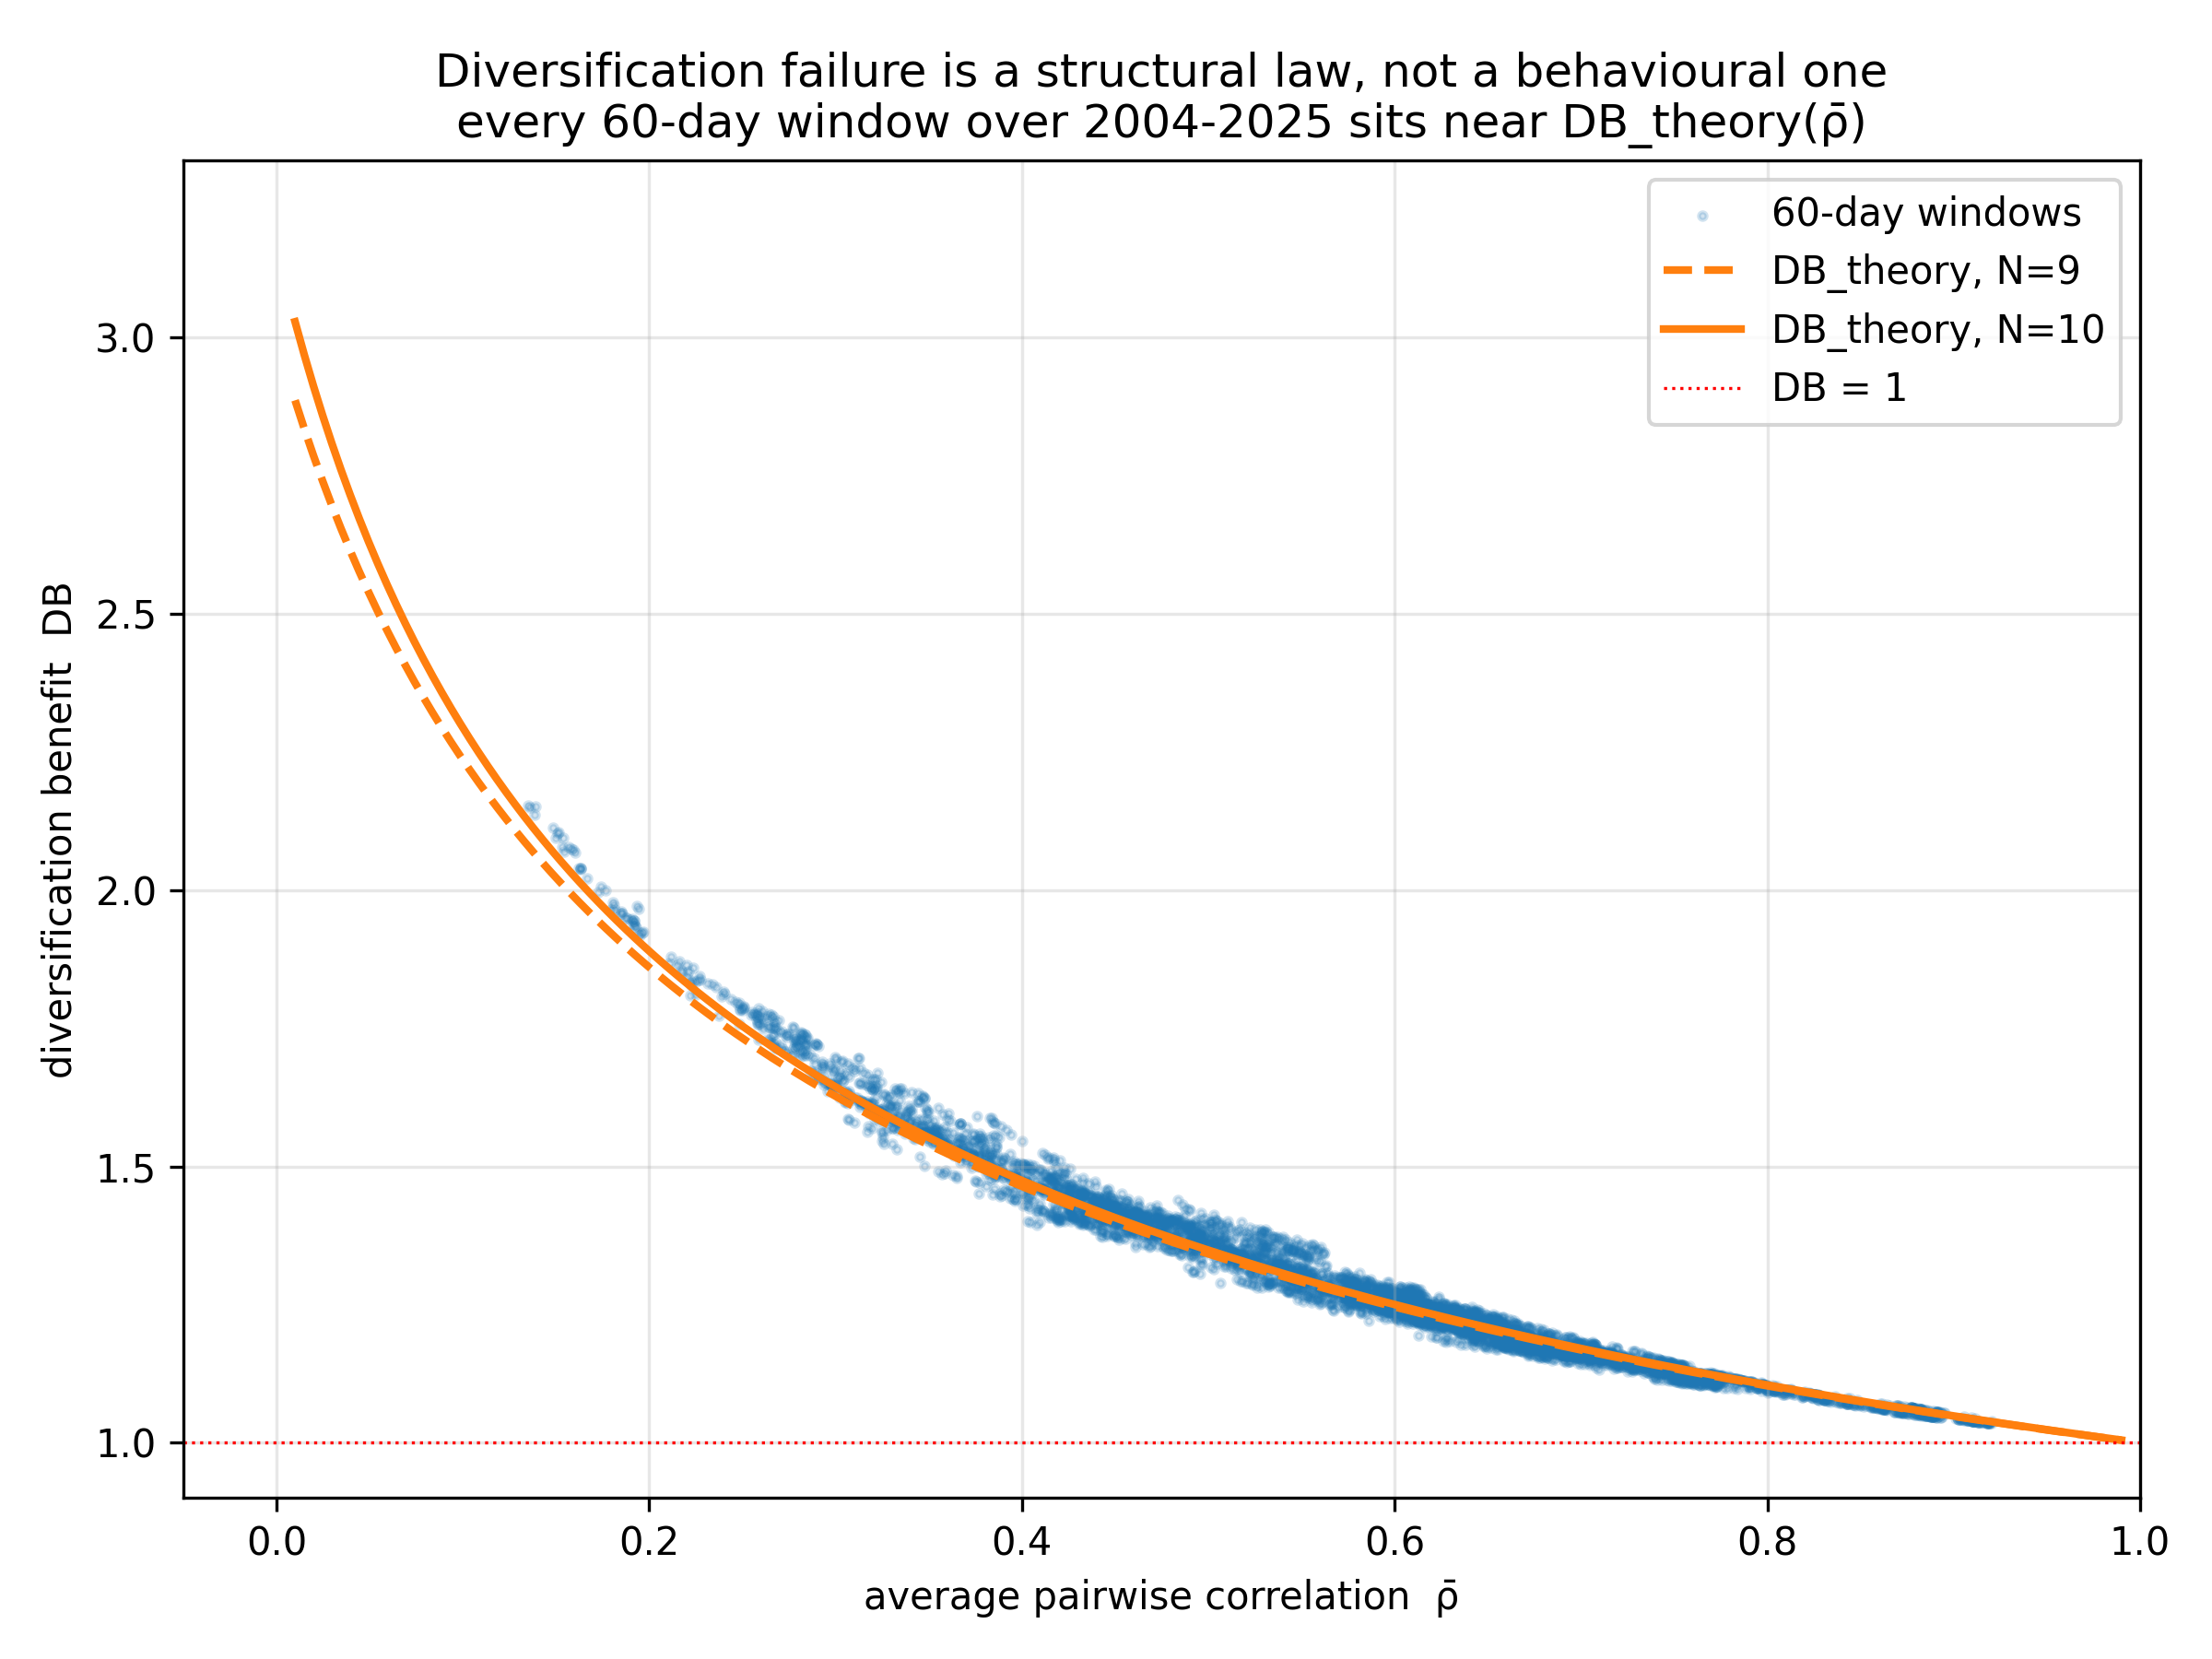
\includegraphics[width=0.95\textwidth]{figures/figS2.png}
\caption{\textit{Structural diversification failure (supporting the ``Empirical setting'' Results subsection).} Diversification benefit DB versus average pairwise correlation ρ̄ across 5,414 sixty-day rolling windows of nine US sector ETFs (XLRE appended on its 2015-10-08 inception, yielding a 10-sector panel post-2015), 30 March 2004 -- 30 December 2025. The theoretical structural curve DB(ρ̄, \emph{N}) = 1 / √(1/\emph{N} + (1 − 1/\emph{N}) ρ̄) is overlaid; mean absolute error of empirical points against the curve is 0.016, with maximum deviation 0.100. Spearman ρ(ρ̄, DB) = --0.993 (\emph{p} \textless{} 10⁻¹⁵). Named crisis episodes (peak ρ̄, minimum DB during the episode): GFC 2008 (0.83, 1.08); Eurozone crisis 2010--12 (0.92, 1.03); China devaluation 2015 (0.80, 1.10); COVID-19 selloff 2020 (0.92, 1.04); inflation shock 2022 (0.74, 1.16). Each crisis sits on the predicted curve. Source file: \protect\path|empirical/figures/diversification_failure_scatter.png|.}
\label{fig:figS2}
\end{figure*}



\begin{figure*}[!htbp]
\centering
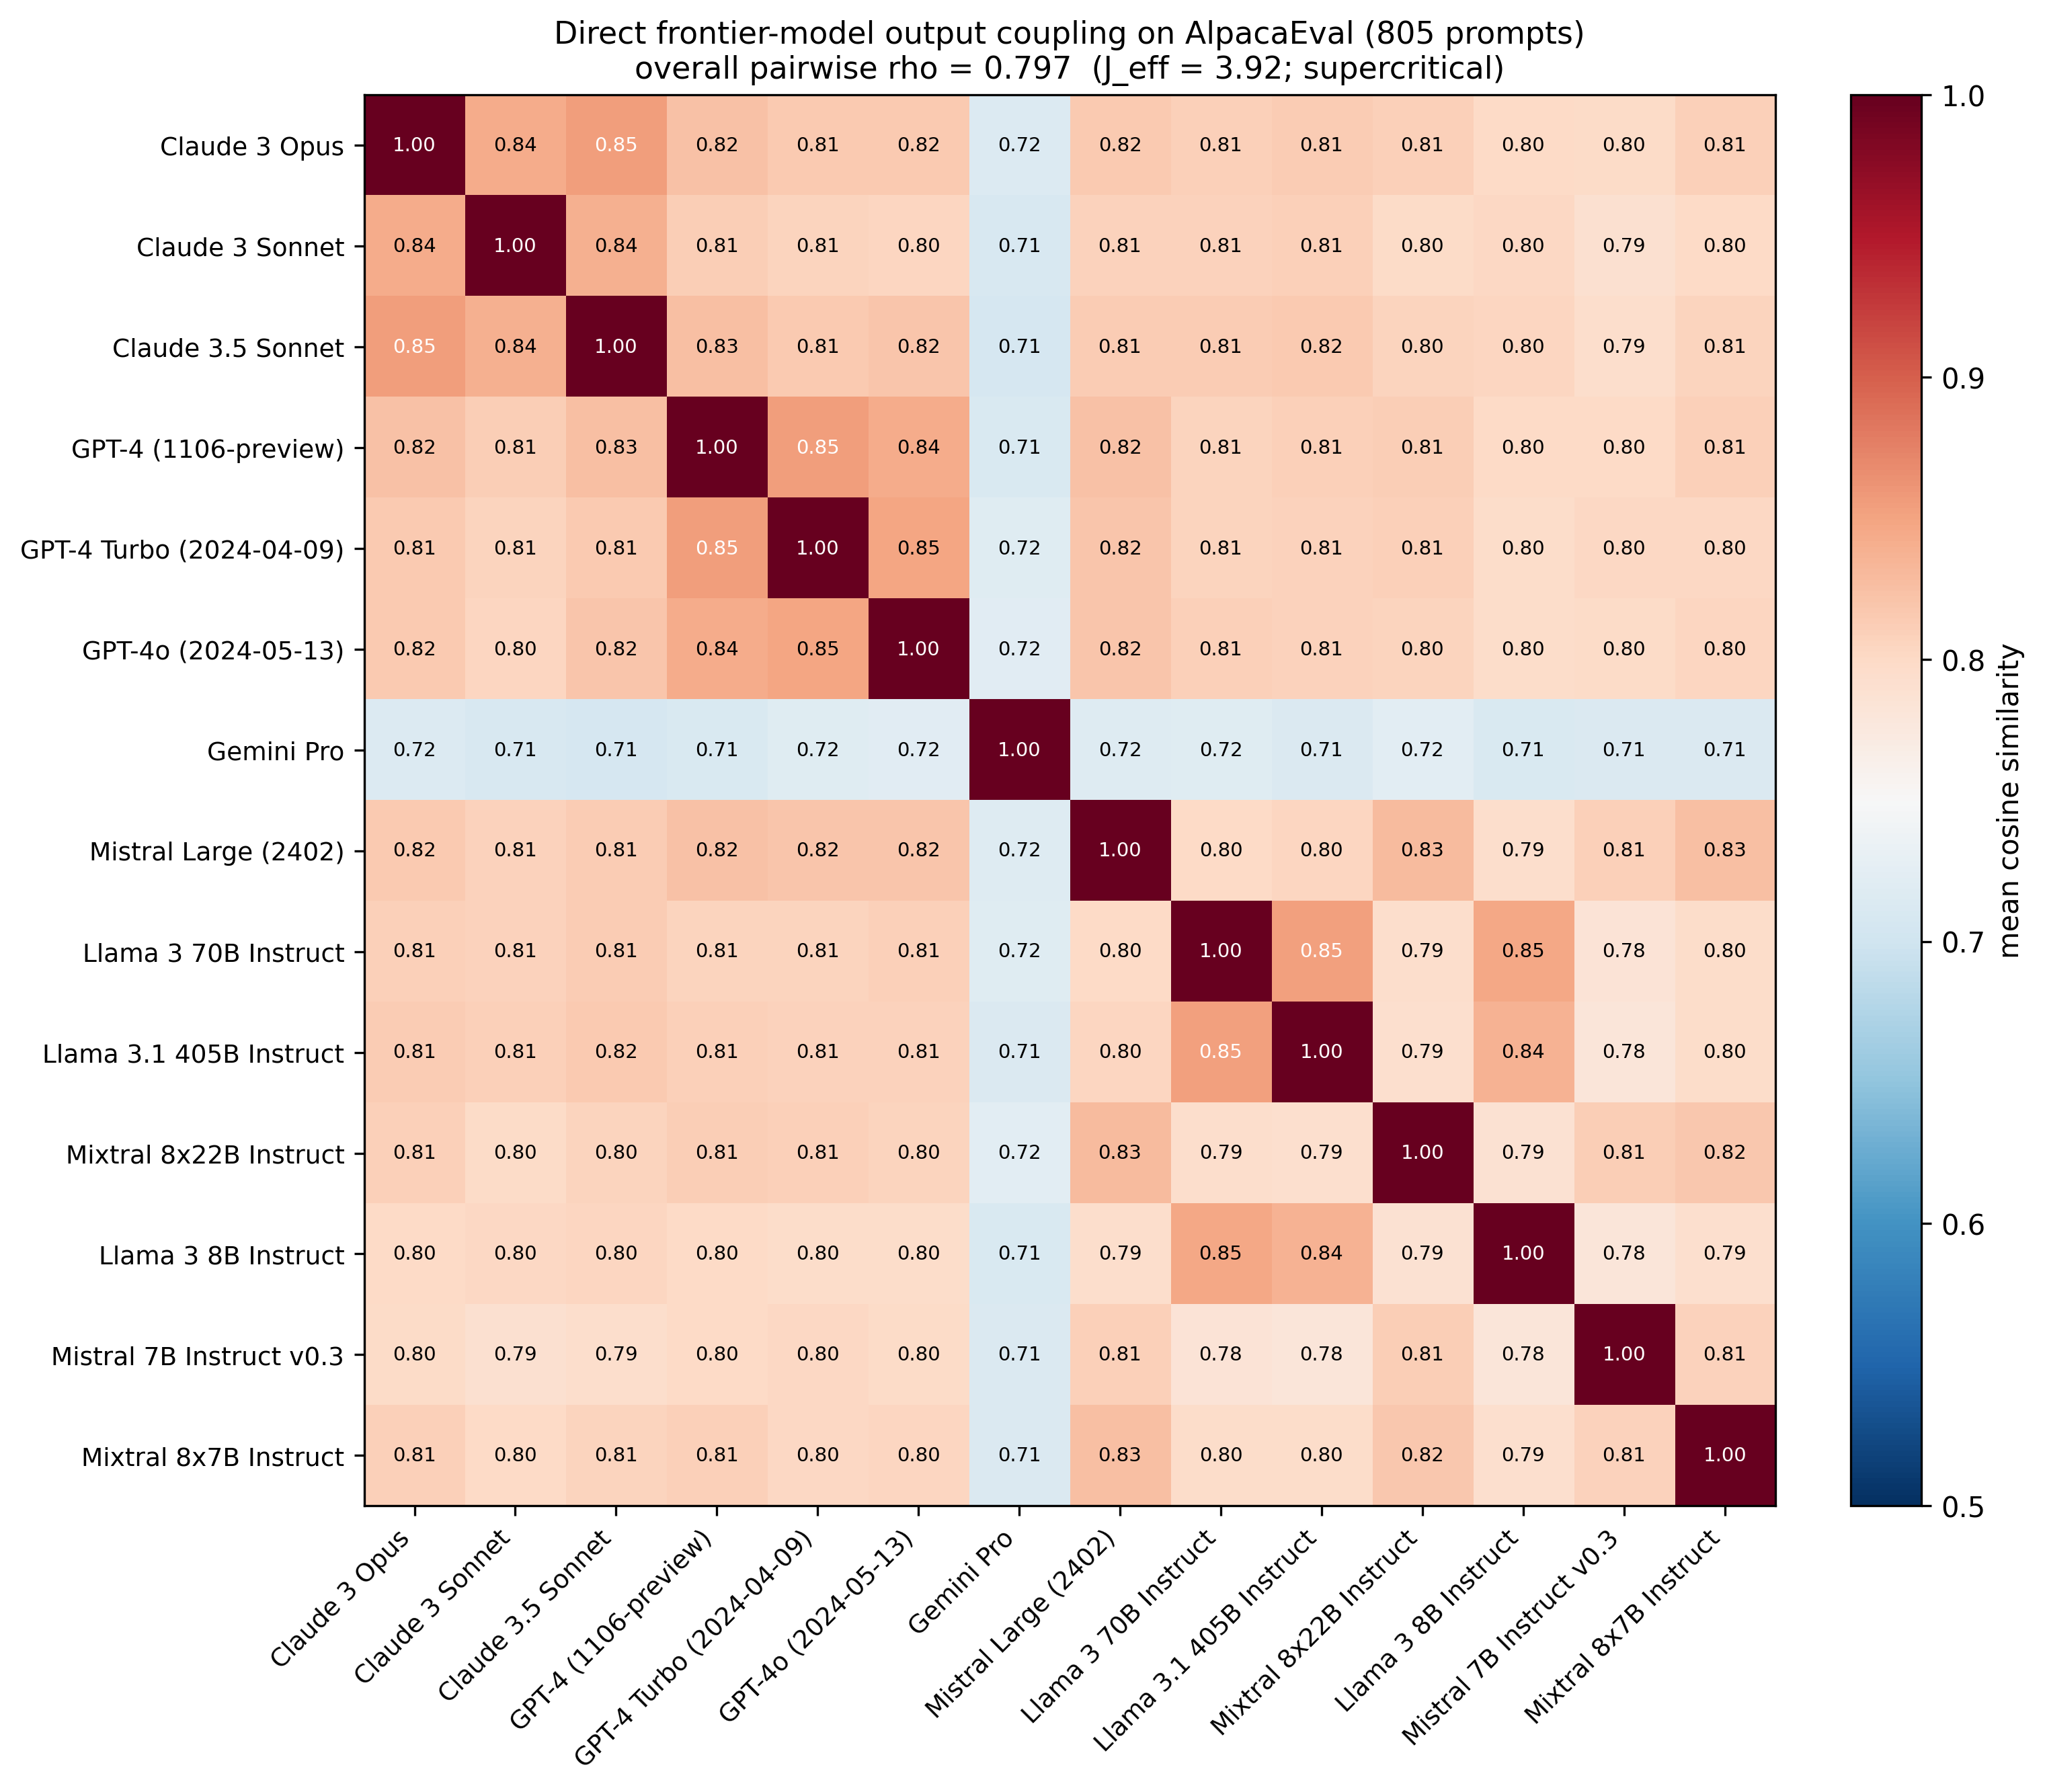
\includegraphics[width=0.95\textwidth]{figures/figS3.png}
\caption{\textit{Direct AI output coupling (supporting the ``AI coupling'' Results subsection).} 14 × 14 pairwise cosine-similarity matrix of sentence-transformer embeddings (\texttt{all-MiniLM-L6-v2}, 384-dim, L2-normalized) of frontier-model responses to 805 shared AlpacaEval v2 prompts \cite{li2023alpacaeval}. Models are grouped by provider --- Anthropic (Claude 3 Opus, Claude 3 Sonnet, Claude 3.5 Sonnet), OpenAI (GPT-4 1106-preview, GPT-4 Turbo 2024-04-09, GPT-4o 2024-05-13), Google (Gemini Pro), and a Mistral / Meta block (Mistral Large 2402, Llama 3 70B, Llama 3.1 405B, Mixtral 8x22B, Llama 3 8B, Mistral 7B v0.3, Mixtral 8x7B). Mean off-diagonal similarity ρ = 0.797, mapping to \emph{J}ₑff = 3.92 under ρ̄ = \emph{J}/(1+\emph{J}). Same-family blocks (e.g., Claude 3 Opus × Claude 3.5 Sonnet) reach ρ ≈ 0.85; cross-family pairs remain at ρ ≈ 0.79, indicating coupling operates across organizational boundaries rather than within model families alone. Source file: \protect\path|empirical/figures/ai_coupling_direct_heatmap.png|.}
\label{fig:figS3}
\end{figure*}



\begin{figure*}[!htbp]
\centering
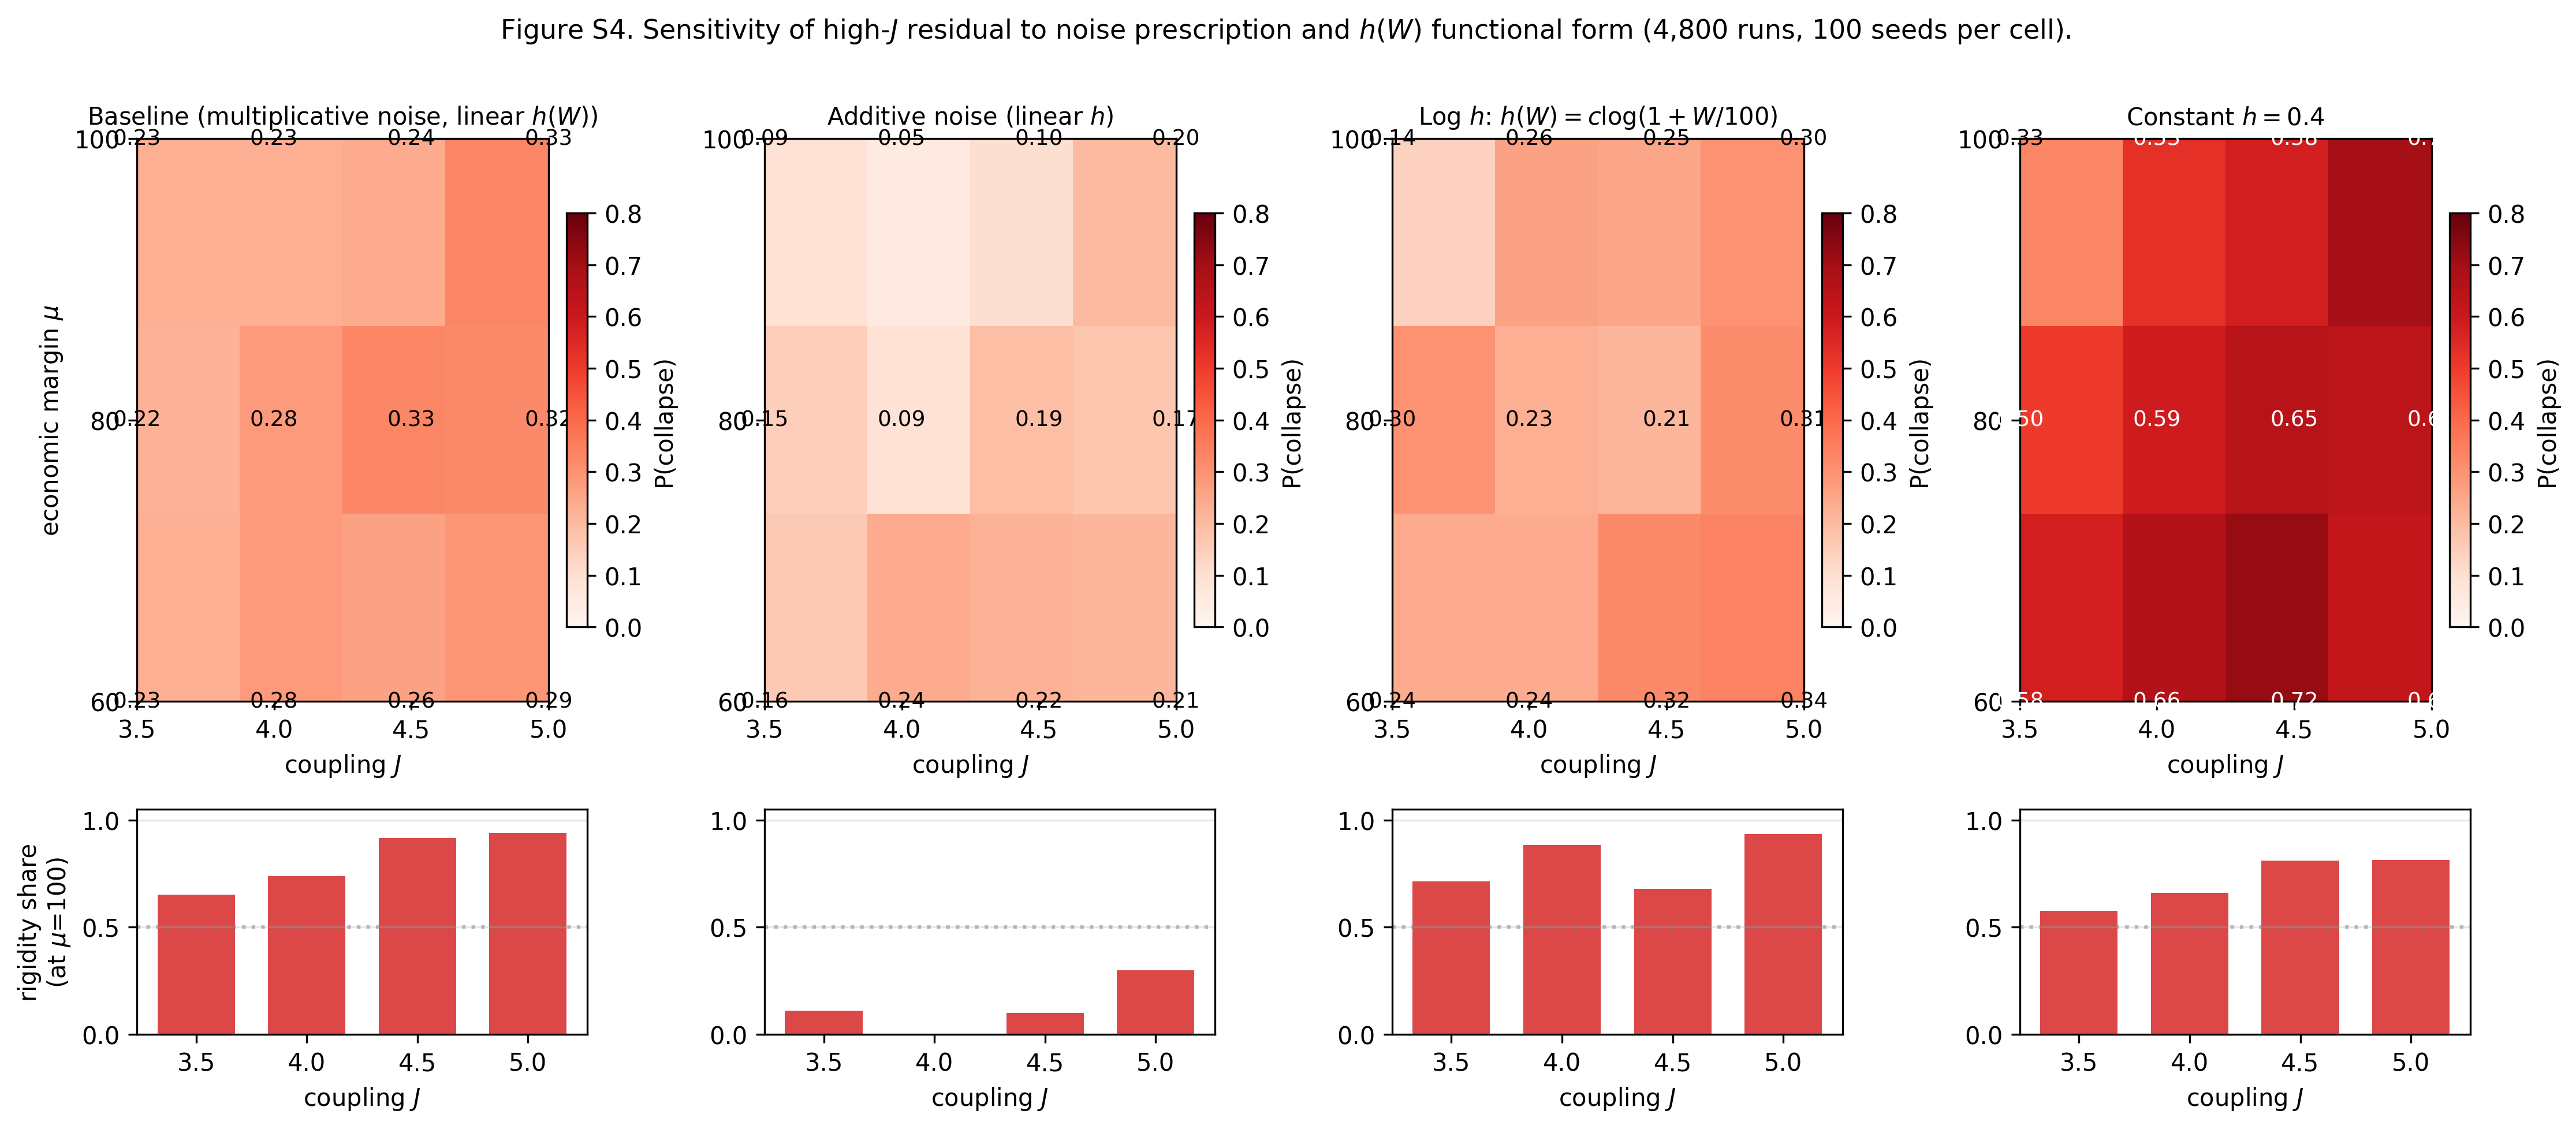
\includegraphics[width=0.95\textwidth]{figures/figS4.png}
\caption{\textit{Sensitivity sweep --- noise prescription and h(W) form (supporting §S5.1).} Top row: P(collapse) heatmap over the high-\emph{J} band (\emph{J} ∈ \{3.5, 4, 4.5, 5\}) × protective-margin band (\emph{μ} ∈ \{60, 80, 100\}) for four model variants --- baseline (multiplicative noise \emph{ξ}√(1−\emph{m}²), linear \emph{h}(\emph{W}) = 2(\emph{W}/500)), additive noise (constant \emph{ξ}, linear \emph{h}), logarithmic \emph{h}(\emph{W}) = 0.577·log(1+\emph{W}/100), and constant \emph{h} = 0.4. Bottom row: rigidity share at \emph{μ} = 100 across the \emph{J} range for each variant. Headline cell (\emph{J} = 5, \emph{μ} = 100): baseline 0.33, additive 0.20, log \emph{h} 0.30, constant \emph{h} 0.70. The qualitative residual is robust to log-vs-linear \emph{h}; constant \emph{h} is substantially worse, ruling out the baseline as a tuned best-case; under additive noise the residual persists but rigidity-typed dominance falls (0.94 → 0.30), confirming the \emph{h}/\emph{J}² landscape result is multiplicative-noise- specific while the asymmetry itself is not. 4,800 runs total (100 seeds per cell × 12 cells × 4 variants). Source files: \protect\path|simulation/scripts/sensitivity_sweep.py|, \protect\path|simulation/results/sensitivity/figure_s4_sensitivity_sweep.png|.}
\label{fig:figS4}
\end{figure*}



\begin{figure*}[!htbp]
\centering
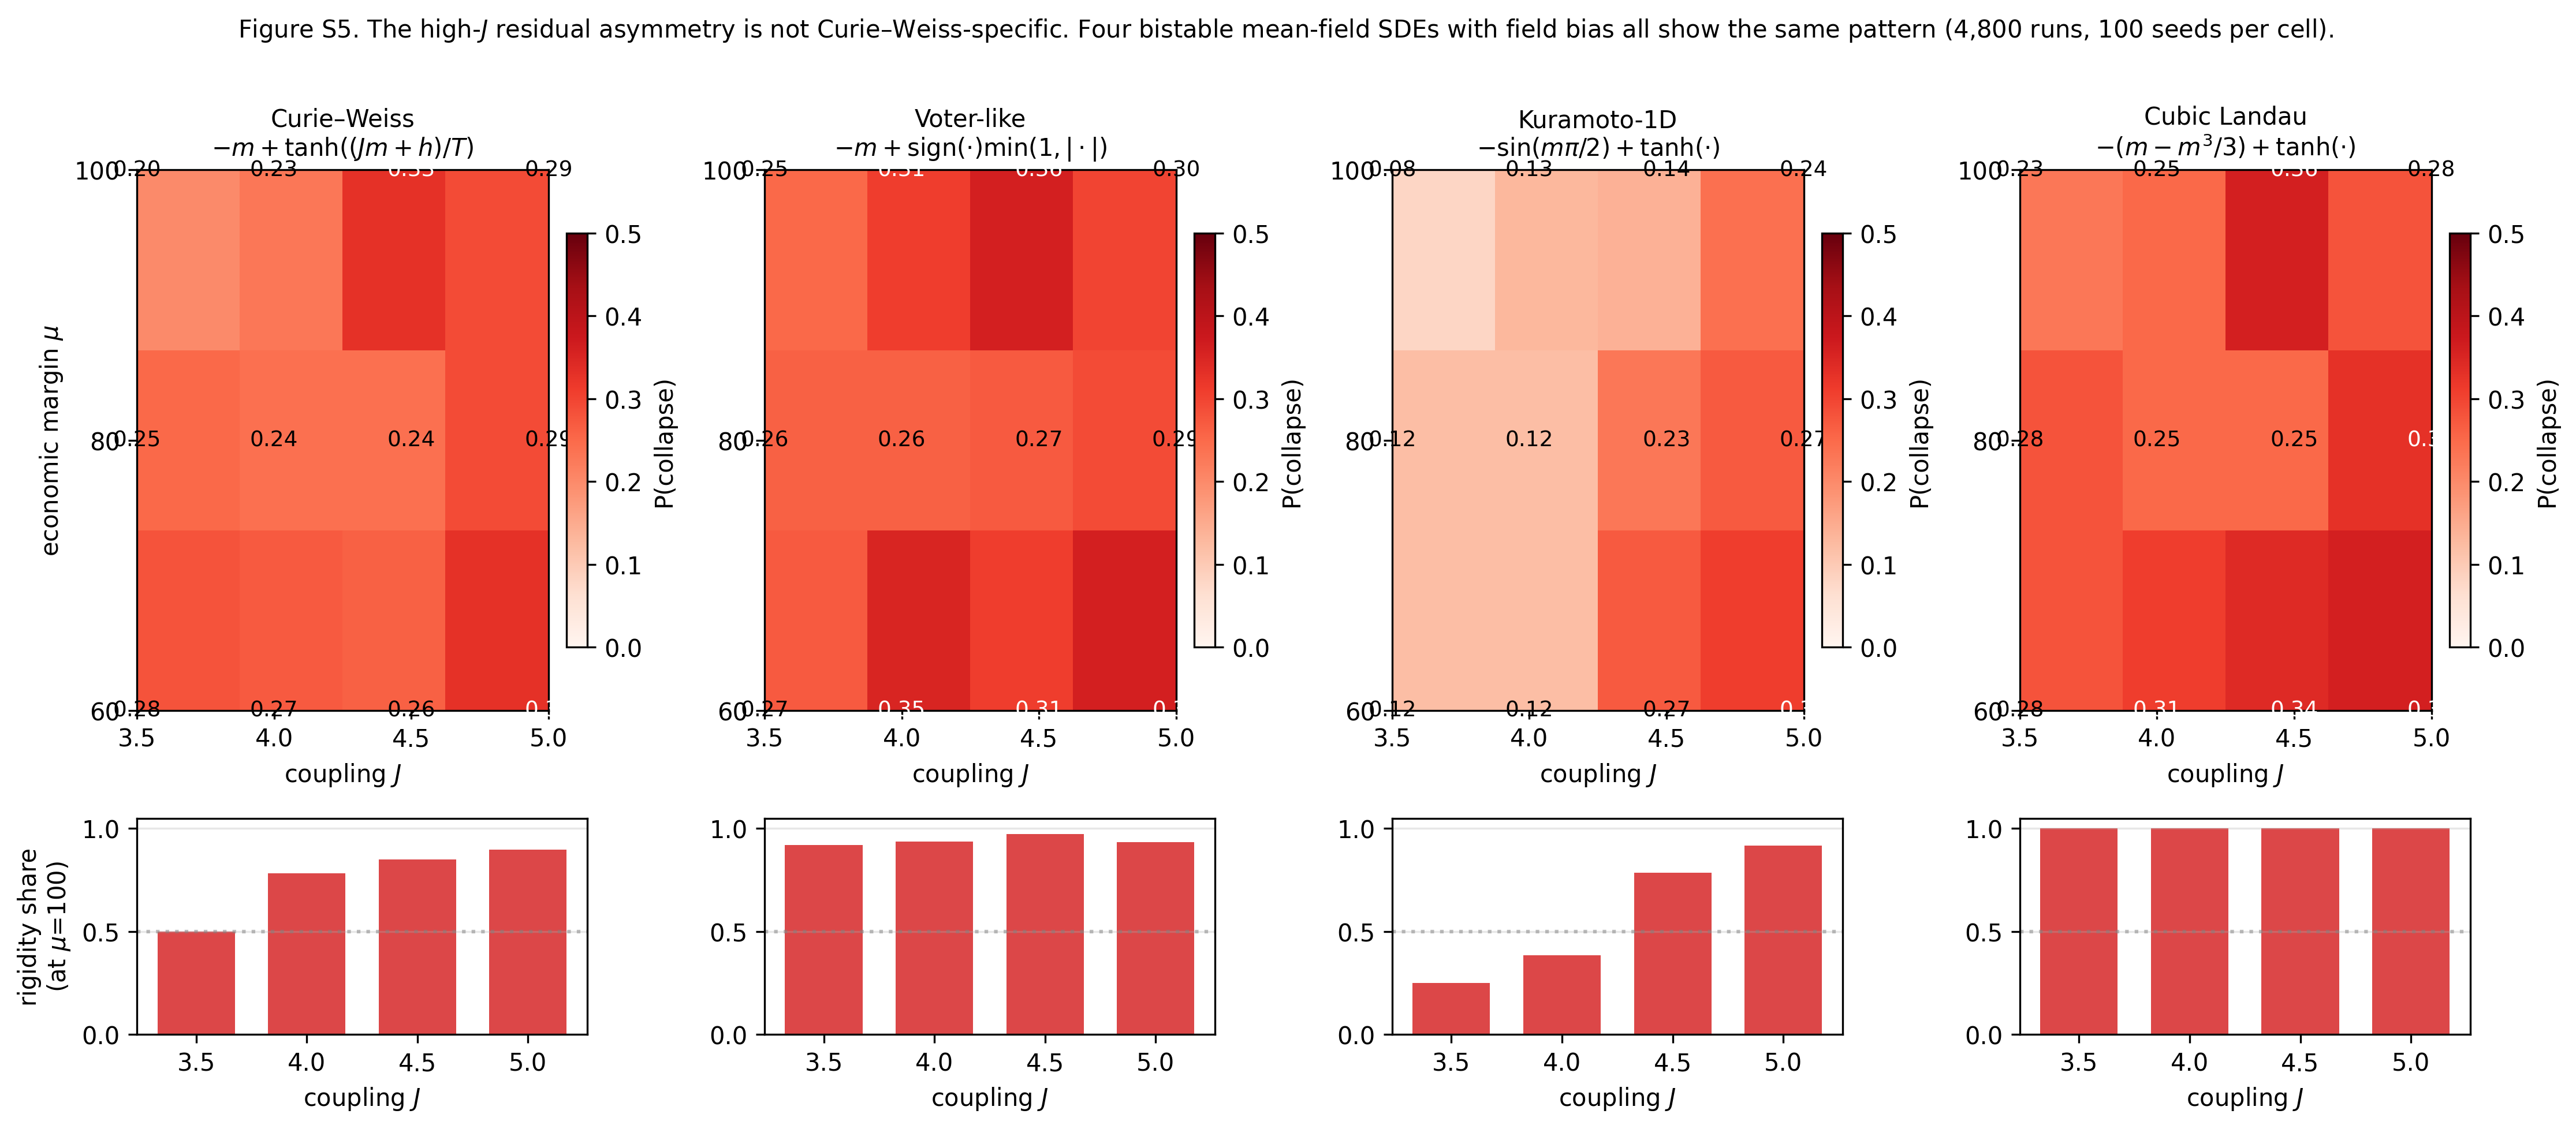
\includegraphics[width=0.95\textwidth]{figures/figS5.png}
\caption{\textit{Alternative-model-class robustness (supporting §S5.3).} Top row: P(collapse) heatmap over the high-\emph{J} band (\emph{J} ∈ \{3.5, 4, 4.5, 5\}) × protective-margin band (\emph{μ} ∈ \{60, 80, 100\}) for four bistable mean-field SDEs sharing the field-bias structure but differing in nonlinearity --- Curie--Weiss tanh, voter-like piecewise sign, Kuramoto-1D sine, cubic Landau. Bottom row: rigidity share at \emph{μ} = 100 across the \emph{J} range. At the headline cell (\emph{J} = 5, \emph{μ} = 100): Curie--Weiss 0.29, voter-like 0.30, Kuramoto-1D 0.24, cubic Landau 0.28 --- a 0.24--0.30 band. The high-\emph{J} residual and rigidity-dominance pattern survive across all four model classes (rigidity share at the headline cell is 0.90 / 0.93 / 0.92 / 1.00 respectively), demonstrating that the asymmetry is generic to bistable mean-field SDEs with field bias rather than specific to Curie--Weiss. 4,800 runs total (100 seeds × 12 cells × 4 variants). Source: \protect\path|simulation/results/alternative_class/figure_s5_alternative_class.png|.}
\label{fig:figS5}
\end{figure*}



\begin{figure*}[!htbp]
\centering
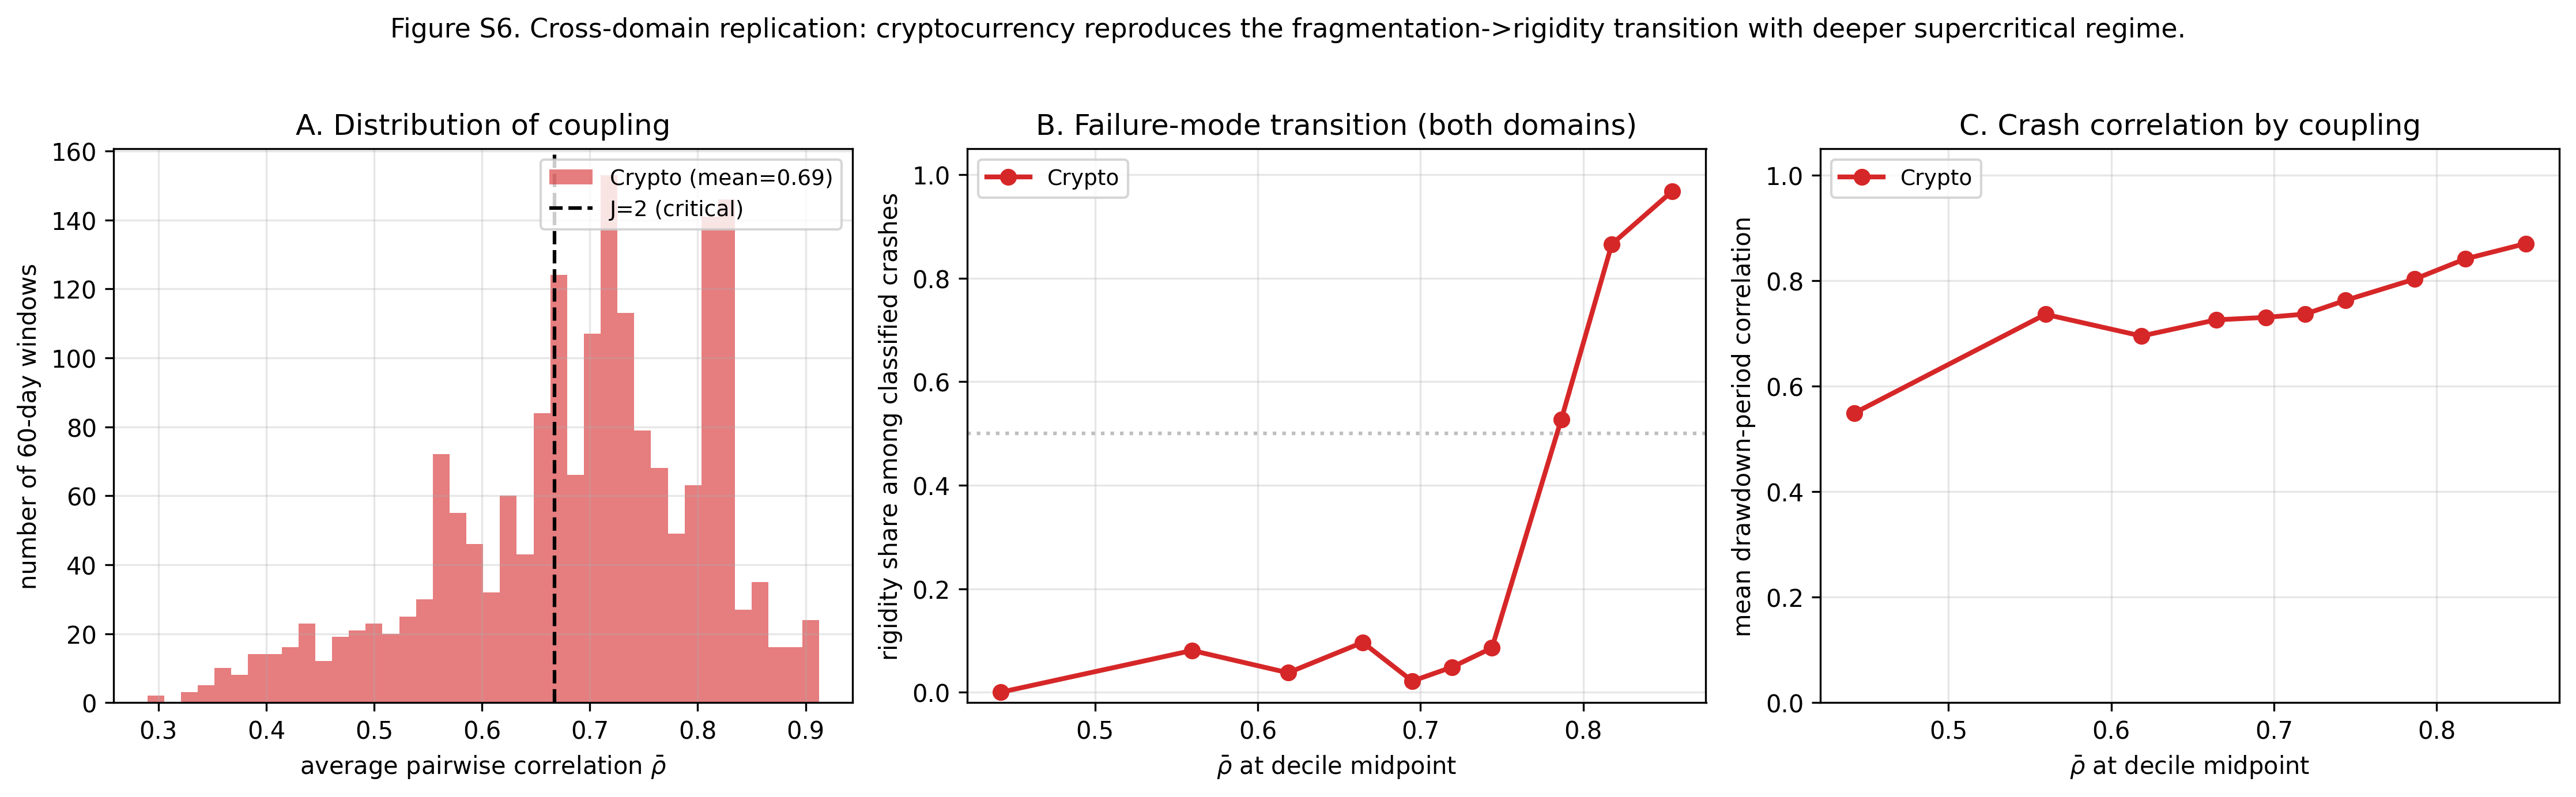
\includegraphics[width=0.95\textwidth]{figures/figS6.png}
\caption{\textit{Cross-domain replication: cryptocurrency markets (supporting §S5.4).} Three panels of the 10-token crypto basket (2020--2025, 1,864 60-day windows). (A) Distribution of average pairwise correlation ρ̄: crypto mean ρ̄ = 0.69 (versus S\&P \textasciitilde0.50, not overplotted), with 64.4\% of crypto windows supercritical (ρ̄ \textgreater{} 0.667, \emph{J} \textgreater{} 2) versus \textasciitilde25\% for S\&P. (B) Failure-mode transition: rigidity share among classified crashes for the crypto basket rises with ρ̄ and crosses 50\% near decile 7 (ρ̄ ≈ 0.79); the S\&P comparator curve is reported in the main text (Figure 8) and is not overplotted here to keep the panels readable. (C) Drawdown-period mean pairwise correlation rises monotonically from 0.55 to 0.87 across crypto deciles. The framework's prediction --- higher-coupling domains exhibit rigidity dominance more readily --- holds at the second domain. Source: \protect\path|empirical/figures/figure_s6_crypto_vs_sp500.png|.}
\label{fig:figS6}
\end{figure*}

\begin{center}\rule{0.5\linewidth}{0.5pt}\end{center}


\end{document}
